% ========================================================================
% Indoor Positioning via Signal Strength Features and Deep Multitask Learning
% IEEE Conference Style Project Report — Five-Member Implementation
% ========================================================================
\documentclass[conference]{IEEEtran}

% -- Packages ------------------------------------------------------------
\usepackage[utf8]{inputenc}
\usepackage[T1]{fontenc}
\usepackage{graphicx}
\usepackage{amsmath,amssymb}
\usepackage{booktabs}
\usepackage{array}
\usepackage{xcolor}
\usepackage{cite}
\usepackage{balance}
\usepackage{tikz}
\usetikzlibrary{arrows.meta,positioning}
\usepackage[hidelinks,breaklinks]{hyperref}
\usepackage{url}
\def\UrlBreaks{\do\/\do-\do.\do_}

% Graphics paths
\graphicspath{{figures/}{../results/figures/}{../outputs/}}

% Avoid bad line breaks in IEEE two-column layout
\hyphenation{fin-ger-print fin-ger-prints lo-cal-i-za-tion multi-task}

% TikZ styles for pipeline figures
\tikzset{
  blk/.style={draw=black!70, rounded corners=2pt, minimum height=10mm,
              minimum width=21mm, text width=19mm, align=center,
              font=\scriptsize, fill=blue!7},
  outblk/.style={blk, fill=green!10},
  arr/.style={-{Stealth[length=2mm]}, thick, black!70}
}

% -- Title & Authors -----------------------------------------------------
\title{Indoor Positioning via Wi-Fi Signal Strength Features and Deep Multitask Learning}

\author{
  \IEEEauthorblockN{Team T076 --- Indoor Wi-Fi Positioning Project}
  \IEEEauthorblockA{Department of Computer Science and Engineering\\
    Five-Member Deep Learning Research Project Report}
}

% ======================================================================
\begin{document}
\maketitle

% -- Abstract --------------------------------------------------------------
\begin{abstract}
Accurate indoor positioning remains a critical challenge for location-based services where Global Navigation Satellite Systems (GNSS) suffer severe attenuation and multi-path degradation. This paper presents a comprehensive, five-member investigation of Wi-Fi fingerprint-based indoor localization on the public UJIIndoorLoc benchmark, which encompasses 21,048 received signal strength indication (RSSI) scans from 520 access points across three multi-floor university buildings. Moving beyond decoupled classical baselines, we formulate a unified deep learning pipeline that simultaneously estimates hierarchical discrete building and floor classes alongside continuous two-dimensional metric coordinates $(x, y)$. 

We evaluate four modeling paradigms on a strictly held-out test set ($N = 1{,}111$) exhibiting a four-month temporal gap and unobserved receiver devices: (i)~classical machine learning baselines ($k$-NN, Random Forest, Extra Trees, XGBoost); (ii)~hard-parameter-sharing multitask deep neural networks (512--256--128 trunk with LayerNorm and GELU activations); (iii)~loss balancing and physical regularization techniques including homoscedastic uncertainty weighting, access-point dropout, and RSSI noise augmentation; and (iv)~a novel two-stage hybrid architecture integrating out-of-fold tree probability stacking with residual gradient boosted decision tree (GBDT) spatial correction. 

Our findings demonstrate that deep continuous manifolds overcome the step-function discretization bottlenecks inherent to decision trees, reducing mean positioning error from 12.30\,m (Random Forest) to 8.95\,m in the multitask network. Furthermore, our Full Hybrid system achieves the best overall performance across all evaluated metrics: 99.82\% building accuracy, 92.08\% floor accuracy, 8.51\,m mean positioning error (6.30\,m median error, $P_{90} = 17.58$\,m), and an EvAAL competition score of 8.96. The complete codebase, preprocessed splits, saved checkpoints, and automated evaluation suites are integrated for full reproducibility.
\end{abstract}

\begin{IEEEkeywords}
Indoor positioning, Wi-Fi fingerprinting, RSSI, deep multitask learning, hybrid ensembles, uncertainty loss weighting, UJIIndoorLoc, EvAAL benchmark.
\end{IEEEkeywords}

% ======================================================================
% SECTION I -- INTRODUCTION (Member 5 Lead)
% ======================================================================
% !TEX root = ../main.tex
% ─────────────────────────────────────────────────────────────────────────────
% Section: Introduction
% Included from main.tex with % !TEX root = ../main.tex
% ─────────────────────────────────────────────────────────────────────────────
% Section: Introduction
% Included from main.tex with % !TEX root = ../main.tex
% ─────────────────────────────────────────────────────────────────────────────
% Section: Introduction
% Included from main.tex with \input{sections/introduction}
% ─────────────────────────────────────────────────────────────────────────────

\label{sec:introduction}

Location-based services (LBS) have become essential to modern commercial, logistical, and emergency operations. While Global Navigation Satellite Systems (GNSS) deliver reliable sub-metre positioning in open outdoor environments, their microwave signals are heavily attenuated, scattered, and blocked by structural building materials such as reinforced concrete, tinted glass, and steel frames~\cite{torres2014ujiindoorloc}. Consequently, satellite-based localization fails in indoor environments where humans spend upwards of 80\% of their daily lives.

To bridge this operational divide, Indoor Positioning Systems (IPS) leverage opportunistic terrestrial radio-frequency (RF) signals. Among available technologies—including Bluetooth Low Energy (BLE), Ultra-Wideband (UWB), and cellular signals—Wireless Local Area Network (WLAN / Wi-Fi) infrastructure stands out due to its ubiquitous presence across campuses, hospitals, transit terminals, and commercial complexes~\cite{feng2022survey}. Utilizing existing IEEE 802.11 access points (APs) avoids the substantial capital cost of deploying specialized hardware anchor nodes.

Rather than relying on explicit radio propagation modeling (such as log-distance path loss or ray tracing)—which requires knowing exact AP coordinates, antenna patterns, and dynamic indoor floor layouts—\emph{fingerprinting} reframes localization as an empirical pattern-recognition problem~\cite{torres2014ujiindoorloc, torres2015comprehensive}. During an offline survey phase, received signal strength indication (RSSI) values from all detectable APs are cataloged at surveyed reference locations to form a radio map. During online operation, an incoming real-time RSSI vector observed by a mobile device is matched against the database or fed to a predictive model to estimate user position.

Despite its practicality, Wi-Fi RSSI fingerprinting presents three fundamental machine-learning challenges:
\begin{enumerate}
    \item \textbf{High Dimensionality and Extreme Sparsity:} In enterprise environments with hundreds of deployed APs, any single scan detects only a small subset of visible transmitters (typically 3--5\%), leaving over 95\% of feature dimensions unobserved~\cite{torres2014ujiindoorloc}.
    \item \textbf{Complex Propagation Dynamics and Device Heterogeneity:} Multipath fading, temporal signal fluctuation, human shadowing, and antenna gain differences across mobile phone vendors distort recorded decibel levels, introducing substantial noise~\cite{torres2015comprehensive}.
    \item \textbf{Coupled Hierarchical Spatial Targets:} An indoor location is not merely a pair of continuous metric coordinates; it possesses discrete topological context—specifically, which building and floor the user occupies. Misclassifying a floor or building results in severe operational failure (e.g., dispatching emergency responders to the wrong level), even if the 2D Euclidean distance error appears deceptively small.
\end{enumerate}

\subsection{Research Gap and Motivation}
In prevailing literature, indoor positioning targets are predominantly addressed in isolation:
\begin{itemize}
    \item \emph{Decoupled Single-Task Models:} Building and floor classification are frequently trained as distinct classifiers (e.g., using $k$-NN, Support Vector Machines, or Random Forests~\cite{salamah2016enhanced}), while metric coordinate regression is handled by completely independent models. Under this decoupled paradigm, the coordinate regression model cannot leverage the rich inductive biases learned by building and floor classifiers.
    \item \emph{Cascaded Hierarchical Pipelines:} Several architectures (e.g.,~\cite{kim2018scalable}) employ a cascading pipeline: a coarse classifier selects a building, a subsequent classifier selects a floor, and a building/floor-specific sub-network regresses $(x, y)$ coordinates. While physically intuitive, cascading systems suffer from catastrophic \emph{error propagation}: an error in the initial building or floor stage irrevocably ruins downstream coordinate estimation.
    \item \emph{Lack of Controlled End-to-End Multitask Benchmarks:} While deep neural networks have demonstrated strong feature extraction capabilities~\cite{nowicki2017low, song2019cnnloc}, there remains a lack of controlled, unified comparisons on standardized public benchmarks that benchmark classical ML against both single-task and unified multi-task deep architectures on identical input representations.
\end{itemize}

Building upon the theoretical foundations of Multitask Learning (MTL) articulated by Caruana~\cite{caruana1997multitask}, related tasks trained in parallel with a shared internal representation benefit from inductive transfer mechanisms: \emph{data amplification}, \emph{eavesdropping}, \emph{attention focusing}, and \emph{representation bias}. In indoor positioning, learning coarse discrete boundaries (buildings and floors) forces hidden representations to encode macro-scale spatial geometry, which can act as a regularizer for fine-grained coordinate regression.

\subsection{Research Questions}
This investigation is guided by four central research questions:
\begin{itemize}
    \item[\textbf{RQ1:}] \emph{Model Baseline Comparison.} How do classical machine learning baselines ($k$-NN, Random Forest, XGBoost) compare against deep neural network architectures across discrete classification (building, floor) and continuous regression (coordinates)?
    \item[\textbf{RQ2:}] \emph{Inductive Transfer in Multitask Learning.} Does a unified hard-parameter-sharing multitask network outperform isolated single-task models in 2D coordinate regression by jointly optimizing building, floor, and coordinate objectives?
    \item[\textbf{RQ3:}] \emph{Metric Discrepancy.} How do discrete classification accuracy and continuous mean positioning error (MPE) interact, and what trade-offs emerge when balancing loss functions between heterogeneous task heads?
    \item[\textbf{RQ4:}] \emph{Robustness to Signal Sparsity.} How resilient are shared representations to extreme unobserved-signal sparsity compared to instance-based and ensemble baselines?
\end{itemize}

\subsection{Research Objectives and Expected Contributions}
To address these research questions, this project undertakes the following specific objectives:
\begin{enumerate}
    \item \textbf{Comprehensive Literature and Theoretical Review:} Systematically review existing classical ML and deep learning methods for Wi-Fi positioning, establishing mathematical formulations for multi-objective loss optimization.
    \item \textbf{Controlled Benchmark Framework:} Construct a standardized evaluation pipeline on the UJIIndoorLoc public benchmark~\cite{torres2014ujiindoorloc}, ensuring zero validation leakage and rigorous comparison across $k$-NN, Random Forest, XGBoost, Single-Task Deep Networks, and Multitask Deep Networks.
    \item \textbf{Unified Multitask Architecture Design:} Design and implement a hard-parameter-sharing neural network capable of simultaneous multi-output inference (building, floor, longitude, latitude) from preprocessed RSSI fingerprints (459 access points observed in the training data, out of 520).
    \item \textbf{Empirical Analysis of Multi-Objective Balancing:} Investigate loss weighting strategies ($\lambda_b, \lambda_f, \lambda_c$) to avoid negative transfer and harmonize categorical cross-entropy with continuous metric regression.
\end{enumerate}

\subsection{Paper Organization}
The remainder of this report is organized as follows: Section~\ref{sec:related-work} reviews related work, comparative taxonomies, and theoretical MTL foundations. Section~\ref{sec:dataset_preprocessing} details the UJIIndoorLoc benchmark, exploratory data analysis, preprocessing and missing-signal handling. Section~\ref{sec:dl_architecture} describes the multitask network and its single-task baselines, Section~\ref{sec:hybrid-methodology} the hybrid stacking and residual-correction methods, and Section~\ref{sec:loss-regularization} the loss-weighting and regularization ablations. Section~\ref{sec:results_evaluation} presents the comparative results and error analysis. Finally, Section~\ref{sec:discussion_conclusion} discusses limitations and concludes the paper with future research directions.

% ─────────────────────────────────────────────────────────────────────────────

\label{sec:introduction}

Location-based services (LBS) have become essential to modern commercial, logistical, and emergency operations. While Global Navigation Satellite Systems (GNSS) deliver reliable sub-metre positioning in open outdoor environments, their microwave signals are heavily attenuated, scattered, and blocked by structural building materials such as reinforced concrete, tinted glass, and steel frames~\cite{torres2014ujiindoorloc}. Consequently, satellite-based localization fails in indoor environments where humans spend upwards of 80\% of their daily lives.

To bridge this operational divide, Indoor Positioning Systems (IPS) leverage opportunistic terrestrial radio-frequency (RF) signals. Among available technologies—including Bluetooth Low Energy (BLE), Ultra-Wideband (UWB), and cellular signals—Wireless Local Area Network (WLAN / Wi-Fi) infrastructure stands out due to its ubiquitous presence across campuses, hospitals, transit terminals, and commercial complexes~\cite{feng2022survey}. Utilizing existing IEEE 802.11 access points (APs) avoids the substantial capital cost of deploying specialized hardware anchor nodes.

Rather than relying on explicit radio propagation modeling (such as log-distance path loss or ray tracing)—which requires knowing exact AP coordinates, antenna patterns, and dynamic indoor floor layouts—\emph{fingerprinting} reframes localization as an empirical pattern-recognition problem~\cite{torres2014ujiindoorloc, torres2015comprehensive}. During an offline survey phase, received signal strength indication (RSSI) values from all detectable APs are cataloged at surveyed reference locations to form a radio map. During online operation, an incoming real-time RSSI vector observed by a mobile device is matched against the database or fed to a predictive model to estimate user position.

Despite its practicality, Wi-Fi RSSI fingerprinting presents three fundamental machine-learning challenges:
\begin{enumerate}
    \item \textbf{High Dimensionality and Extreme Sparsity:} In enterprise environments with hundreds of deployed APs, any single scan detects only a small subset of visible transmitters (typically 3--5\%), leaving over 95\% of feature dimensions unobserved~\cite{torres2014ujiindoorloc}.
    \item \textbf{Complex Propagation Dynamics and Device Heterogeneity:} Multipath fading, temporal signal fluctuation, human shadowing, and antenna gain differences across mobile phone vendors distort recorded decibel levels, introducing substantial noise~\cite{torres2015comprehensive}.
    \item \textbf{Coupled Hierarchical Spatial Targets:} An indoor location is not merely a pair of continuous metric coordinates; it possesses discrete topological context—specifically, which building and floor the user occupies. Misclassifying a floor or building results in severe operational failure (e.g., dispatching emergency responders to the wrong level), even if the 2D Euclidean distance error appears deceptively small.
\end{enumerate}

\subsection{Research Gap and Motivation}
In prevailing literature, indoor positioning targets are predominantly addressed in isolation:
\begin{itemize}
    \item \emph{Decoupled Single-Task Models:} Building and floor classification are frequently trained as distinct classifiers (e.g., using $k$-NN, Support Vector Machines, or Random Forests~\cite{salamah2016enhanced}), while metric coordinate regression is handled by completely independent models. Under this decoupled paradigm, the coordinate regression model cannot leverage the rich inductive biases learned by building and floor classifiers.
    \item \emph{Cascaded Hierarchical Pipelines:} Several architectures (e.g.,~\cite{kim2018scalable}) employ a cascading pipeline: a coarse classifier selects a building, a subsequent classifier selects a floor, and a building/floor-specific sub-network regresses $(x, y)$ coordinates. While physically intuitive, cascading systems suffer from catastrophic \emph{error propagation}: an error in the initial building or floor stage irrevocably ruins downstream coordinate estimation.
    \item \emph{Lack of Controlled End-to-End Multitask Benchmarks:} While deep neural networks have demonstrated strong feature extraction capabilities~\cite{nowicki2017low, song2019cnnloc}, there remains a lack of controlled, unified comparisons on standardized public benchmarks that benchmark classical ML against both single-task and unified multi-task deep architectures on identical input representations.
\end{itemize}

Building upon the theoretical foundations of Multitask Learning (MTL) articulated by Caruana~\cite{caruana1997multitask}, related tasks trained in parallel with a shared internal representation benefit from inductive transfer mechanisms: \emph{data amplification}, \emph{eavesdropping}, \emph{attention focusing}, and \emph{representation bias}. In indoor positioning, learning coarse discrete boundaries (buildings and floors) forces hidden representations to encode macro-scale spatial geometry, which can act as a regularizer for fine-grained coordinate regression.

\subsection{Research Questions}
This investigation is guided by four central research questions:
\begin{itemize}
    \item[\textbf{RQ1:}] \emph{Model Baseline Comparison.} How do classical machine learning baselines ($k$-NN, Random Forest, XGBoost) compare against deep neural network architectures across discrete classification (building, floor) and continuous regression (coordinates)?
    \item[\textbf{RQ2:}] \emph{Inductive Transfer in Multitask Learning.} Does a unified hard-parameter-sharing multitask network outperform isolated single-task models in 2D coordinate regression by jointly optimizing building, floor, and coordinate objectives?
    \item[\textbf{RQ3:}] \emph{Metric Discrepancy.} How do discrete classification accuracy and continuous mean positioning error (MPE) interact, and what trade-offs emerge when balancing loss functions between heterogeneous task heads?
    \item[\textbf{RQ4:}] \emph{Robustness to Signal Sparsity.} How resilient are shared representations to extreme unobserved-signal sparsity compared to instance-based and ensemble baselines?
\end{itemize}

\subsection{Research Objectives and Expected Contributions}
To address these research questions, this project undertakes the following specific objectives:
\begin{enumerate}
    \item \textbf{Comprehensive Literature and Theoretical Review:} Systematically review existing classical ML and deep learning methods for Wi-Fi positioning, establishing mathematical formulations for multi-objective loss optimization.
    \item \textbf{Controlled Benchmark Framework:} Construct a standardized evaluation pipeline on the UJIIndoorLoc public benchmark~\cite{torres2014ujiindoorloc}, ensuring zero validation leakage and rigorous comparison across $k$-NN, Random Forest, XGBoost, Single-Task Deep Networks, and Multitask Deep Networks.
    \item \textbf{Unified Multitask Architecture Design:} Design and implement a hard-parameter-sharing neural network capable of simultaneous multi-output inference (building, floor, longitude, latitude) from preprocessed RSSI fingerprints (459 access points observed in the training data, out of 520).
    \item \textbf{Empirical Analysis of Multi-Objective Balancing:} Investigate loss weighting strategies ($\lambda_b, \lambda_f, \lambda_c$) to avoid negative transfer and harmonize categorical cross-entropy with continuous metric regression.
\end{enumerate}

\subsection{Paper Organization}
The remainder of this report is organized as follows: Section~\ref{sec:related-work} reviews related work, comparative taxonomies, and theoretical MTL foundations. Section~\ref{sec:dataset_preprocessing} details the UJIIndoorLoc benchmark, exploratory data analysis, preprocessing and missing-signal handling. Section~\ref{sec:dl_architecture} describes the multitask network and its single-task baselines, Section~\ref{sec:hybrid-methodology} the hybrid stacking and residual-correction methods, and Section~\ref{sec:loss-regularization} the loss-weighting and regularization ablations. Section~\ref{sec:results_evaluation} presents the comparative results and error analysis. Finally, Section~\ref{sec:discussion_conclusion} discusses limitations and concludes the paper with future research directions.

% ─────────────────────────────────────────────────────────────────────────────

\label{sec:introduction}

Location-based services (LBS) have become essential to modern commercial, logistical, and emergency operations. While Global Navigation Satellite Systems (GNSS) deliver reliable sub-metre positioning in open outdoor environments, their microwave signals are heavily attenuated, scattered, and blocked by structural building materials such as reinforced concrete, tinted glass, and steel frames~\cite{torres2014ujiindoorloc}. Consequently, satellite-based localization fails in indoor environments where humans spend upwards of 80\% of their daily lives.

To bridge this operational divide, Indoor Positioning Systems (IPS) leverage opportunistic terrestrial radio-frequency (RF) signals. Among available technologies—including Bluetooth Low Energy (BLE), Ultra-Wideband (UWB), and cellular signals—Wireless Local Area Network (WLAN / Wi-Fi) infrastructure stands out due to its ubiquitous presence across campuses, hospitals, transit terminals, and commercial complexes~\cite{feng2022survey}. Utilizing existing IEEE 802.11 access points (APs) avoids the substantial capital cost of deploying specialized hardware anchor nodes.

Rather than relying on explicit radio propagation modeling (such as log-distance path loss or ray tracing)—which requires knowing exact AP coordinates, antenna patterns, and dynamic indoor floor layouts—\emph{fingerprinting} reframes localization as an empirical pattern-recognition problem~\cite{torres2014ujiindoorloc, torres2015comprehensive}. During an offline survey phase, received signal strength indication (RSSI) values from all detectable APs are cataloged at surveyed reference locations to form a radio map. During online operation, an incoming real-time RSSI vector observed by a mobile device is matched against the database or fed to a predictive model to estimate user position.

Despite its practicality, Wi-Fi RSSI fingerprinting presents three fundamental machine-learning challenges:
\begin{enumerate}
    \item \textbf{High Dimensionality and Extreme Sparsity:} In enterprise environments with hundreds of deployed APs, any single scan detects only a small subset of visible transmitters (typically 3--5\%), leaving over 95\% of feature dimensions unobserved~\cite{torres2014ujiindoorloc}.
    \item \textbf{Complex Propagation Dynamics and Device Heterogeneity:} Multipath fading, temporal signal fluctuation, human shadowing, and antenna gain differences across mobile phone vendors distort recorded decibel levels, introducing substantial noise~\cite{torres2015comprehensive}.
    \item \textbf{Coupled Hierarchical Spatial Targets:} An indoor location is not merely a pair of continuous metric coordinates; it possesses discrete topological context—specifically, which building and floor the user occupies. Misclassifying a floor or building results in severe operational failure (e.g., dispatching emergency responders to the wrong level), even if the 2D Euclidean distance error appears deceptively small.
\end{enumerate}

\subsection{Research Gap and Motivation}
In prevailing literature, indoor positioning targets are predominantly addressed in isolation:
\begin{itemize}
    \item \emph{Decoupled Single-Task Models:} Building and floor classification are frequently trained as distinct classifiers (e.g., using $k$-NN, Support Vector Machines, or Random Forests~\cite{salamah2016enhanced}), while metric coordinate regression is handled by completely independent models. Under this decoupled paradigm, the coordinate regression model cannot leverage the rich inductive biases learned by building and floor classifiers.
    \item \emph{Cascaded Hierarchical Pipelines:} Several architectures (e.g.,~\cite{kim2018scalable}) employ a cascading pipeline: a coarse classifier selects a building, a subsequent classifier selects a floor, and a building/floor-specific sub-network regresses $(x, y)$ coordinates. While physically intuitive, cascading systems suffer from catastrophic \emph{error propagation}: an error in the initial building or floor stage irrevocably ruins downstream coordinate estimation.
    \item \emph{Lack of Controlled End-to-End Multitask Benchmarks:} While deep neural networks have demonstrated strong feature extraction capabilities~\cite{nowicki2017low, song2019cnnloc}, there remains a lack of controlled, unified comparisons on standardized public benchmarks that benchmark classical ML against both single-task and unified multi-task deep architectures on identical input representations.
\end{itemize}

Building upon the theoretical foundations of Multitask Learning (MTL) articulated by Caruana~\cite{caruana1997multitask}, related tasks trained in parallel with a shared internal representation benefit from inductive transfer mechanisms: \emph{data amplification}, \emph{eavesdropping}, \emph{attention focusing}, and \emph{representation bias}. In indoor positioning, learning coarse discrete boundaries (buildings and floors) forces hidden representations to encode macro-scale spatial geometry, which can act as a regularizer for fine-grained coordinate regression.

\subsection{Research Questions}
This investigation is guided by four central research questions:
\begin{itemize}
    \item[\textbf{RQ1:}] \emph{Model Baseline Comparison.} How do classical machine learning baselines ($k$-NN, Random Forest, XGBoost) compare against deep neural network architectures across discrete classification (building, floor) and continuous regression (coordinates)?
    \item[\textbf{RQ2:}] \emph{Inductive Transfer in Multitask Learning.} Does a unified hard-parameter-sharing multitask network outperform isolated single-task models in 2D coordinate regression by jointly optimizing building, floor, and coordinate objectives?
    \item[\textbf{RQ3:}] \emph{Metric Discrepancy.} How do discrete classification accuracy and continuous mean positioning error (MPE) interact, and what trade-offs emerge when balancing loss functions between heterogeneous task heads?
    \item[\textbf{RQ4:}] \emph{Robustness to Signal Sparsity.} How resilient are shared representations to extreme unobserved-signal sparsity compared to instance-based and ensemble baselines?
\end{itemize}

\subsection{Research Objectives and Expected Contributions}
To address these research questions, this project undertakes the following specific objectives:
\begin{enumerate}
    \item \textbf{Comprehensive Literature and Theoretical Review:} Systematically review existing classical ML and deep learning methods for Wi-Fi positioning, establishing mathematical formulations for multi-objective loss optimization.
    \item \textbf{Controlled Benchmark Framework:} Construct a standardized evaluation pipeline on the UJIIndoorLoc public benchmark~\cite{torres2014ujiindoorloc}, ensuring zero validation leakage and rigorous comparison across $k$-NN, Random Forest, XGBoost, Single-Task Deep Networks, and Multitask Deep Networks.
    \item \textbf{Unified Multitask Architecture Design:} Design and implement a hard-parameter-sharing neural network capable of simultaneous multi-output inference (building, floor, longitude, latitude) from preprocessed RSSI fingerprints (459 access points observed in the training data, out of 520).
    \item \textbf{Empirical Analysis of Multi-Objective Balancing:} Investigate loss weighting strategies ($\lambda_b, \lambda_f, \lambda_c$) to avoid negative transfer and harmonize categorical cross-entropy with continuous metric regression.
\end{enumerate}

\subsection{Paper Organization}
The remainder of this report is organized as follows: Section~\ref{sec:related-work} reviews related work, comparative taxonomies, and theoretical MTL foundations. Section~\ref{sec:dataset_preprocessing} details the UJIIndoorLoc benchmark, exploratory data analysis, preprocessing and missing-signal handling. Section~\ref{sec:dl_architecture} describes the multitask network and its single-task baselines, Section~\ref{sec:hybrid-methodology} the hybrid stacking and residual-correction methods, and Section~\ref{sec:loss-regularization} the loss-weighting and regularization ablations. Section~\ref{sec:results_evaluation} presents the comparative results and error analysis. Finally, Section~\ref{sec:discussion_conclusion} discusses limitations and concludes the paper with future research directions.


% ======================================================================
% SECTION II -- RELATED WORK (Member 5 Lead)
% ======================================================================
% !TEX root = ../main.tex
% ─────────────────────────────────────────────────────────────────────────────
% Section: Related Work and Theoretical Foundation
% Included from main.tex with % !TEX root = ../main.tex
% ─────────────────────────────────────────────────────────────────────────────
% Section: Related Work and Theoretical Foundation
% Included from main.tex with % !TEX root = ../main.tex
% ─────────────────────────────────────────────────────────────────────────────
% Section: Related Work and Theoretical Foundation
% Included from main.tex with \input{sections/related_work}
% ─────────────────────────────────────────────────────────────────────────────

\label{sec:related-work}

Indoor positioning via Wi-Fi fingerprinting has evolved significantly over the past two decades. This section synthesizes existing research across instance-based matching, ensemble learning, and deep learning architectures, contrasts their characteristics, and establishes the theoretical foundations of multitask learning.

\subsection{Wi-Fi RSSI Fingerprinting and Instance-Based Baselines}
The foundational paradigm for Wi-Fi localization was pioneered by RADAR~\cite{torres2014ujiindoorloc}, which demonstrated that RF signal vectors observed from fixed transmitters correlate with spatial coordinates. Fingerprinting operates without time-synchronization hardware or explicit line-of-sight propagation modeling by decomposing positioning into an offline radio-map survey and an online pattern-matching phase.

Among instance-based techniques, $k$-Nearest Neighbors ($k$-NN) and Weighted $k$-Nearest Neighbors (WKNN) remain the standard benchmarks. Given an incoming fingerprint $\mathbf{x}$, WKNN calculates signal-space distances $d(\mathbf{x}, \mathbf{x}_i)$ against all stored fingerprints $\mathbf{x}_i$ in the radio map $\mathcal{D}_{\text{train}}$, selects the $k$ nearest exemplars, and predicts coordinates as:
\begin{equation}
    \hat{\mathbf{y}}_c = \sum_{i=1}^k w_i \mathbf{y}_{c,i}, \quad w_i = \frac{1 / (d(\mathbf{x}, \mathbf{x}_i) + \epsilon)}{\sum_{j=1}^k 1 / (d(\mathbf{x}, \mathbf{x}_j) + \epsilon)}
\end{equation}
Torres-Sospedra et al.~\cite{torres2015comprehensive} conducted an exhaustive evaluation of 21 distance and similarity metrics on the UJIIndoorLoc dataset~\cite{torres2014ujiindoorloc}, confirming that non-linear and normalized distance formulations (such as Sørensen and Manhattan distances) often outperform raw Euclidean distance in sparse, high-dimensional RSSI space. However, instance-based methods suffer from high computational complexity during inference ($\mathcal{O}(M \cdot N)$ where $M$ is the radio-map size and $N$ is the number of WAPs), large memory footprints on edge devices, and an inability to learn abstract invariant representations across heterogeneous devices.

\subsection{Tree-Based Ensembles: Random Forest and Gradient Boosting}
To overcome the sensitivity of $k$-NN to noise and outliers, tree-based ensemble methods have gained widespread adoption. Random Forests (RF) construct ensembles of decorrelated decision trees via bootstrap aggregation and random subspace feature selection. Decision trees possess characteristics well matched to RF signals:
\begin{enumerate}
    \item \textbf{Non-Monotonic Boundary Partitioning:} Trees naturally isolate unobserved sentinel indicators (e.g., $+100$ dBm or $-110$ dBm) from active measurements ($-104$ to $0$ dBm) using single axis-aligned splits.
    \item \textbf{Variance Reduction:} Averaging predictions across hundreds of stochastic trees suppresses the high variance introduced by human body shadowing and multipath fluctuations.
    \item \textbf{Intrinsic Feature Selection:} Impurity-based metrics identify which subsets of APs uniquely resolve specific campus zones.
\end{enumerate}
Salamah et al.~\cite{salamah2016enhanced} demonstrated that pairing Random Forest with Principal Component Analysis (PCA) achieved high zone classification accuracy while reducing feature dimensionality and computational training overhead by over 70\%.

Gradient Boosted Decision Trees (GBDT), notably XGBoost, refine this paradigm by training shallow trees sequentially to minimize an arbitrary differentiable loss function via second-order Taylor approximations. XGBoost incorporates explicit regularization ($\ell_1$ and $\ell_2$ penalties on leaf weights) and dedicated sparsity-aware split finding, which dynamically directs missing or unobserved access point values to the default branch that maximizes gain.

\subsection{Deep Learning for Wi-Fi Fingerprinting}
With the advent of deep learning, neural architectures have been applied to capture complex non-linear interactions across large WAP arrays without manual feature engineering~\cite{feng2022survey}.
Nowicki and Wietrzykowski~\cite{nowicki2017low} demonstrated that deep multilayer perceptrons (MLP) trained with stacked autoencoders achieved near-perfect building and floor classification on UJIIndoorLoc, demonstrating that deep hidden layers can extract robust topological representations despite device diversity.

Song et al.~\cite{song2019cnnloc} proposed CNNLoc, reformulating 1D RSSI vectors into multi-channel or spatial representations to leverage 1D/2D Convolutional Neural Networks (CNNs). Their work demonstrated that local convolutional filters capture spatial signal correlation across adjacent AP groups, reducing mean positioning error compared to traditional shallow baselines. A comprehensive survey by Feng et al.~\cite{feng2022survey} highlights that while deep networks consistently outperform classical ML in representation capacity, existing approaches overwhelmingly target either classification or regression separately, or cascade them sequentially.

\subsection{Hierarchical and Multitask Positioning Architectures}
Because indoor locations naturally exhibit hierarchical structure (building $\to$ floor $\to$ 2D coordinates), several works have attempted multi-stage localization. Kim et al.~\cite{kim2018scalable} proposed a scalable hierarchical DNN for UJIIndoorLoc consisting of stacked autoencoders and a decision tree hierarchy. In their system, an initial classifier determines the building, routing the sample to a building-specific floor classifier, which in turn routes the sample to a local coordinate regression model. While this hierarchical decomposition reduces the complexity of each sub-model, it is inherently vulnerable to \emph{error compounding}: an early misclassification in building or floor assignment guarantees a catastrophic localization failure in metric coordinates.

\subsection{Theoretical Foundations of Multitask Learning}
Multitask Learning (MTL) provides a principled machine learning paradigm to model related targets jointly without cascading error propagation. As formalized by Caruana~\cite{caruana1997multitask}, MTL improves generalization performance by training multiple related tasks in parallel using a shared representation.

\begin{figure}[!t]
\centering
% Conceptual schematic of Hard Parameter Sharing Architecture
\begin{minipage}{0.95\columnwidth}
\centering
\fbox{\parbox{0.9\columnwidth}{\centering \small
\textbf{Hard Parameter Sharing MTL Architecture}\\[4pt]
\texttt{Input:} $\mathbf{x} \in \mathbb{R}^{520}$ (Preprocessed RSSI Vector)\\[2pt]
$\Downarrow$\\[2pt]
\textbf{Shared Encoder} $\mathbf{z} = g(\mathbf{x}; \mathbf{\Theta}_{\text{shared}})$\\
(Dense $\to$ BatchNorm $\to$ ReLU $\to$ Dropout layers)\\[2pt]
$\swarrow$ \hspace{28pt} $\Downarrow$ \hspace{28pt} $\searrow$\\[2pt]
\textbf{Head 1:} Building \quad \textbf{Head 2:} Floor \quad \textbf{Head 3:} Coordinates\\
$\hat{\mathbf{y}}_b = \text{Softmax}(\mathbf{W}_b \mathbf{z})$ \quad $\hat{\mathbf{y}}_f = \text{Softmax}(\mathbf{W}_f \mathbf{z})$ \quad $\hat{\mathbf{y}}_c = \mathbf{W}_c \mathbf{z} + \mathbf{b}_c$
}}
\end{minipage}
\caption{Conceptual schema of the hard-parameter-sharing multitask architecture for simultaneous building, floor, and coordinate estimation.}
\label{fig:mtl-arch}
\end{figure}

In hard parameter sharing (Figure~\ref{fig:mtl-arch}), the initial hidden layers are shared across all tasks, while task-specific heads branch out near the output. Caruana identified four key inductive mechanisms enabled by shared representations:
\begin{enumerate}
    \item \textbf{Data Amplification:} Samples informative for floor differentiation also tune the shared feature extractor for coordinate regression, effectively increasing the statistical sample size.
    \item \textbf{Eavesdropping:} Tasks with subtle target gradients can ``eavesdrop'' on representations optimized by tasks with cleaner objective landscapes (e.g., coarse building boundaries).
    \item \textbf{Attention Focusing:} Shared optimization penalizes representations that overfit to transient noise on irrelevant WAPs, focusing feature weights on APs that exhibit consistent mutual information across all spatial targets.
    \item \textbf{Representation Bias:} MTL biases the hypothesis search space toward compact representations that simultaneously explain discrete regional topology and metric spatial geometry.
\end{enumerate}

\subsection{Mathematical Problem Formulation}
Let a single preprocessed Wi-Fi fingerprint be represented as a vector $\mathbf{x} = [x_1, x_2, \dots, x_N]^T \in \mathbb{R}^N$, where $N = 520$ denotes the total number of cataloged wireless access points in the environment.

Each observation is paired with three ground-truth spatial targets:
\begin{itemize}
    \item \textbf{Building Label ($y_b$):} A discrete multiclass index $y_b \in \{0, 1, 2\}$, representing $B = 3$ campus buildings.
    \item \textbf{Floor Level ($y_f$):} A discrete multiclass index $y_f \in \{0, 1, 2, 3, 4\}$, representing $F = 5$ vertical levels.
    \item \textbf{Spatial Coordinates ($\mathbf{y}_c$):} A continuous bivariate vector $\mathbf{y}_c = [x_{\text{long}}, y_{\text{lat}}]^T \in \mathbb{R}^2$ expressed in projected metric UTM coordinates.
\end{itemize}

\subsubsection{Multi-Objective Loss Formulation}
In the unified multitask network, the total empirical risk objective is defined as a weighted combination of task-specific loss functions:
\begin{equation}
    \mathcal{L}_{\text{total}}(\mathbf{\Theta}) = \lambda_b \mathcal{L}_b(\hat{\mathbf{y}}_b, y_b) + \lambda_f \mathcal{L}_f(\hat{\mathbf{y}}_f, y_f) + \lambda_c \mathcal{L}_c(\hat{\mathbf{y}}_c, \mathbf{y}_c)
    \label{eq:mtl-loss}
\end{equation}
where $\lambda_b, \lambda_f, \lambda_c > 0$ are task-balancing hyperparameters.

The classification objectives are governed by categorical cross-entropy losses:
\begin{align}
    \mathcal{L}_b &= -\sum_{k=0}^{B-1} \mathbb{I}(y_b = k) \log \hat{P}(y_b = k \mid \mathbf{x}) \\
    \mathcal{L}_f &= -\sum_{k=0}^{F-1} \mathbb{I}(y_f = k) \log \hat{P}(y_f = k \mid \mathbf{x})
\end{align}
For coordinate regression, the loss is computed as the Mean Squared Error (MSE) over normalized metric coordinates:
\begin{equation}
    \mathcal{L}_c = \frac{1}{2} \|\hat{\mathbf{y}}_c - \mathbf{y}_c\|_2^2 = \frac{1}{2} \left[ (\hat{x}_{\text{long}} - x_{\text{long}})^2 + (\hat{y}_{\text{lat}} - y_{\text{lat}})^2 \right]
\end{equation}

\subsubsection{Loss Balancing and Gradient Harmony}
A central theoretical challenge in multitask learning is loss-scale disparity~\cite{chen2018gradnorm, ruder2017overview}. Categorical cross-entropy values typically range in magnitude from $0.1$ to $2.0$. If coordinates are evaluated in unnormalized raw metres ($x \sim 10^5\text{ m}$ in UTM projection), coordinate regression gradients dwarf classification gradients by multiple orders of magnitude, causing severe negative transfer and model collapse. To guarantee balanced optimization, coordinates must be normalized (via min-max or z-score standard scaling), and task weights ($\lambda_b, \lambda_f, \lambda_c$) must be calibrated to ensure balanced gradient norms across shared encoder layers.

\subsection{Comparative Summary of Existing Approaches}
Table~\ref{tab:lit-matrix} provides a structured comparison of representative Wi-Fi indoor positioning methodologies in the literature, positioning our proposed multitask approach against prior works.

\begin{table*}[!t]
\centering
\caption{Systematic Comparison of Wi-Fi Positioning Methodologies in Prior Literature}
\label{tab:lit-matrix}
\begin{tabular}{lp{3.4cm}p{2.6cm}p{3.2cm}p{3.8cm}}
\toprule
\textbf{Approach / Reference} & \textbf{Prediction Targets} & \textbf{Evaluation Metrics} & \textbf{Key Strengths} & \textbf{Identified Limitations} \\
\midrule
$k$-NN / WKNN \newline \cite{torres2014ujiindoorloc, torres2015comprehensive} & 
Coordinates $(x, y)$, \newline Building, Floor & 
Mean Positioning Error (m), Accuracy (\%) & 
Non-parametric; zero training phase; robust empirical baseline. & 
$\mathcal{O}(M)$ inference time; large memory footprint; no latent feature abstraction. \\
\midrule
Random Forest + PCA \newline \cite{salamah2016enhanced} & 
Room / Zone Classification & 
Classification Accuracy (\%), Execution Time & 
Robust to RSSI noise; PCA reduces feature dimensionality by 70\%. & 
Evaluated on private dataset; targets discrete zones only; no continuous regression. \\
\midrule
Stacked Autoencoders + MLP \newline \cite{nowicki2017low} & 
Building, Floor & 
Classification Hit Rate (\%) & 
Unsupervised feature pretraining; highly accurate topological prediction. & 
Does not predict continuous $(x, y)$ coordinates; lacks metric localization. \\
\midrule
Hierarchical Deep Neural Net \newline \cite{kim2018scalable} & 
Building $\to$ Floor $\to$ \newline Coordinates $(x, y)$ & 
Mean Positioning Error (m), Accuracy (\%) & 
Scalable modular architecture; separates coarse from fine prediction. & 
Cascading pipeline propagates early classification errors to coordinate regression. \\
\midrule
1D/2D CNN (CNNLoc) \newline \cite{song2019cnnloc} & 
Floor, Coordinates $(x, y)$ & 
Mean Positioning Error (m), Cumulative Error CDF & 
Convolutional filters capture local spatial correlations across AP channels. & 
Separate models for floor and coordinates; does not exploit joint MTL regularization. \\
\midrule
\textbf{Proposed Multitask Net} \newline (Our Investigation) & 
\textbf{Simultaneous Building, \newline Floor, and Coordinates} & 
\textbf{Accuracy (\%), MPE (m), \newline CDF Percentiles, IPIN Error} & 
\textbf{Shared latent representation; inductive transfer; single-pass multi-target inference.} & 
\textbf{Requires careful multi-objective loss balancing to prevent negative transfer.} \\
\bottomrule
\end{tabular}
\end{table*}

% ─────────────────────────────────────────────────────────────────────────────

\label{sec:related-work}

Indoor positioning via Wi-Fi fingerprinting has evolved significantly over the past two decades. This section synthesizes existing research across instance-based matching, ensemble learning, and deep learning architectures, contrasts their characteristics, and establishes the theoretical foundations of multitask learning.

\subsection{Wi-Fi RSSI Fingerprinting and Instance-Based Baselines}
The foundational paradigm for Wi-Fi localization was pioneered by RADAR~\cite{torres2014ujiindoorloc}, which demonstrated that RF signal vectors observed from fixed transmitters correlate with spatial coordinates. Fingerprinting operates without time-synchronization hardware or explicit line-of-sight propagation modeling by decomposing positioning into an offline radio-map survey and an online pattern-matching phase.

Among instance-based techniques, $k$-Nearest Neighbors ($k$-NN) and Weighted $k$-Nearest Neighbors (WKNN) remain the standard benchmarks. Given an incoming fingerprint $\mathbf{x}$, WKNN calculates signal-space distances $d(\mathbf{x}, \mathbf{x}_i)$ against all stored fingerprints $\mathbf{x}_i$ in the radio map $\mathcal{D}_{\text{train}}$, selects the $k$ nearest exemplars, and predicts coordinates as:
\begin{equation}
    \hat{\mathbf{y}}_c = \sum_{i=1}^k w_i \mathbf{y}_{c,i}, \quad w_i = \frac{1 / (d(\mathbf{x}, \mathbf{x}_i) + \epsilon)}{\sum_{j=1}^k 1 / (d(\mathbf{x}, \mathbf{x}_j) + \epsilon)}
\end{equation}
Torres-Sospedra et al.~\cite{torres2015comprehensive} conducted an exhaustive evaluation of 21 distance and similarity metrics on the UJIIndoorLoc dataset~\cite{torres2014ujiindoorloc}, confirming that non-linear and normalized distance formulations (such as Sørensen and Manhattan distances) often outperform raw Euclidean distance in sparse, high-dimensional RSSI space. However, instance-based methods suffer from high computational complexity during inference ($\mathcal{O}(M \cdot N)$ where $M$ is the radio-map size and $N$ is the number of WAPs), large memory footprints on edge devices, and an inability to learn abstract invariant representations across heterogeneous devices.

\subsection{Tree-Based Ensembles: Random Forest and Gradient Boosting}
To overcome the sensitivity of $k$-NN to noise and outliers, tree-based ensemble methods have gained widespread adoption. Random Forests (RF) construct ensembles of decorrelated decision trees via bootstrap aggregation and random subspace feature selection. Decision trees possess characteristics well matched to RF signals:
\begin{enumerate}
    \item \textbf{Non-Monotonic Boundary Partitioning:} Trees naturally isolate unobserved sentinel indicators (e.g., $+100$ dBm or $-110$ dBm) from active measurements ($-104$ to $0$ dBm) using single axis-aligned splits.
    \item \textbf{Variance Reduction:} Averaging predictions across hundreds of stochastic trees suppresses the high variance introduced by human body shadowing and multipath fluctuations.
    \item \textbf{Intrinsic Feature Selection:} Impurity-based metrics identify which subsets of APs uniquely resolve specific campus zones.
\end{enumerate}
Salamah et al.~\cite{salamah2016enhanced} demonstrated that pairing Random Forest with Principal Component Analysis (PCA) achieved high zone classification accuracy while reducing feature dimensionality and computational training overhead by over 70\%.

Gradient Boosted Decision Trees (GBDT), notably XGBoost, refine this paradigm by training shallow trees sequentially to minimize an arbitrary differentiable loss function via second-order Taylor approximations. XGBoost incorporates explicit regularization ($\ell_1$ and $\ell_2$ penalties on leaf weights) and dedicated sparsity-aware split finding, which dynamically directs missing or unobserved access point values to the default branch that maximizes gain.

\subsection{Deep Learning for Wi-Fi Fingerprinting}
With the advent of deep learning, neural architectures have been applied to capture complex non-linear interactions across large WAP arrays without manual feature engineering~\cite{feng2022survey}.
Nowicki and Wietrzykowski~\cite{nowicki2017low} demonstrated that deep multilayer perceptrons (MLP) trained with stacked autoencoders achieved near-perfect building and floor classification on UJIIndoorLoc, demonstrating that deep hidden layers can extract robust topological representations despite device diversity.

Song et al.~\cite{song2019cnnloc} proposed CNNLoc, reformulating 1D RSSI vectors into multi-channel or spatial representations to leverage 1D/2D Convolutional Neural Networks (CNNs). Their work demonstrated that local convolutional filters capture spatial signal correlation across adjacent AP groups, reducing mean positioning error compared to traditional shallow baselines. A comprehensive survey by Feng et al.~\cite{feng2022survey} highlights that while deep networks consistently outperform classical ML in representation capacity, existing approaches overwhelmingly target either classification or regression separately, or cascade them sequentially.

\subsection{Hierarchical and Multitask Positioning Architectures}
Because indoor locations naturally exhibit hierarchical structure (building $\to$ floor $\to$ 2D coordinates), several works have attempted multi-stage localization. Kim et al.~\cite{kim2018scalable} proposed a scalable hierarchical DNN for UJIIndoorLoc consisting of stacked autoencoders and a decision tree hierarchy. In their system, an initial classifier determines the building, routing the sample to a building-specific floor classifier, which in turn routes the sample to a local coordinate regression model. While this hierarchical decomposition reduces the complexity of each sub-model, it is inherently vulnerable to \emph{error compounding}: an early misclassification in building or floor assignment guarantees a catastrophic localization failure in metric coordinates.

\subsection{Theoretical Foundations of Multitask Learning}
Multitask Learning (MTL) provides a principled machine learning paradigm to model related targets jointly without cascading error propagation. As formalized by Caruana~\cite{caruana1997multitask}, MTL improves generalization performance by training multiple related tasks in parallel using a shared representation.

\begin{figure}[!t]
\centering
% Conceptual schematic of Hard Parameter Sharing Architecture
\begin{minipage}{0.95\columnwidth}
\centering
\fbox{\parbox{0.9\columnwidth}{\centering \small
\textbf{Hard Parameter Sharing MTL Architecture}\\[4pt]
\texttt{Input:} $\mathbf{x} \in \mathbb{R}^{520}$ (Preprocessed RSSI Vector)\\[2pt]
$\Downarrow$\\[2pt]
\textbf{Shared Encoder} $\mathbf{z} = g(\mathbf{x}; \mathbf{\Theta}_{\text{shared}})$\\
(Dense $\to$ BatchNorm $\to$ ReLU $\to$ Dropout layers)\\[2pt]
$\swarrow$ \hspace{28pt} $\Downarrow$ \hspace{28pt} $\searrow$\\[2pt]
\textbf{Head 1:} Building \quad \textbf{Head 2:} Floor \quad \textbf{Head 3:} Coordinates\\
$\hat{\mathbf{y}}_b = \text{Softmax}(\mathbf{W}_b \mathbf{z})$ \quad $\hat{\mathbf{y}}_f = \text{Softmax}(\mathbf{W}_f \mathbf{z})$ \quad $\hat{\mathbf{y}}_c = \mathbf{W}_c \mathbf{z} + \mathbf{b}_c$
}}
\end{minipage}
\caption{Conceptual schema of the hard-parameter-sharing multitask architecture for simultaneous building, floor, and coordinate estimation.}
\label{fig:mtl-arch}
\end{figure}

In hard parameter sharing (Figure~\ref{fig:mtl-arch}), the initial hidden layers are shared across all tasks, while task-specific heads branch out near the output. Caruana identified four key inductive mechanisms enabled by shared representations:
\begin{enumerate}
    \item \textbf{Data Amplification:} Samples informative for floor differentiation also tune the shared feature extractor for coordinate regression, effectively increasing the statistical sample size.
    \item \textbf{Eavesdropping:} Tasks with subtle target gradients can ``eavesdrop'' on representations optimized by tasks with cleaner objective landscapes (e.g., coarse building boundaries).
    \item \textbf{Attention Focusing:} Shared optimization penalizes representations that overfit to transient noise on irrelevant WAPs, focusing feature weights on APs that exhibit consistent mutual information across all spatial targets.
    \item \textbf{Representation Bias:} MTL biases the hypothesis search space toward compact representations that simultaneously explain discrete regional topology and metric spatial geometry.
\end{enumerate}

\subsection{Mathematical Problem Formulation}
Let a single preprocessed Wi-Fi fingerprint be represented as a vector $\mathbf{x} = [x_1, x_2, \dots, x_N]^T \in \mathbb{R}^N$, where $N = 520$ denotes the total number of cataloged wireless access points in the environment.

Each observation is paired with three ground-truth spatial targets:
\begin{itemize}
    \item \textbf{Building Label ($y_b$):} A discrete multiclass index $y_b \in \{0, 1, 2\}$, representing $B = 3$ campus buildings.
    \item \textbf{Floor Level ($y_f$):} A discrete multiclass index $y_f \in \{0, 1, 2, 3, 4\}$, representing $F = 5$ vertical levels.
    \item \textbf{Spatial Coordinates ($\mathbf{y}_c$):} A continuous bivariate vector $\mathbf{y}_c = [x_{\text{long}}, y_{\text{lat}}]^T \in \mathbb{R}^2$ expressed in projected metric UTM coordinates.
\end{itemize}

\subsubsection{Multi-Objective Loss Formulation}
In the unified multitask network, the total empirical risk objective is defined as a weighted combination of task-specific loss functions:
\begin{equation}
    \mathcal{L}_{\text{total}}(\mathbf{\Theta}) = \lambda_b \mathcal{L}_b(\hat{\mathbf{y}}_b, y_b) + \lambda_f \mathcal{L}_f(\hat{\mathbf{y}}_f, y_f) + \lambda_c \mathcal{L}_c(\hat{\mathbf{y}}_c, \mathbf{y}_c)
    \label{eq:mtl-loss}
\end{equation}
where $\lambda_b, \lambda_f, \lambda_c > 0$ are task-balancing hyperparameters.

The classification objectives are governed by categorical cross-entropy losses:
\begin{align}
    \mathcal{L}_b &= -\sum_{k=0}^{B-1} \mathbb{I}(y_b = k) \log \hat{P}(y_b = k \mid \mathbf{x}) \\
    \mathcal{L}_f &= -\sum_{k=0}^{F-1} \mathbb{I}(y_f = k) \log \hat{P}(y_f = k \mid \mathbf{x})
\end{align}
For coordinate regression, the loss is computed as the Mean Squared Error (MSE) over normalized metric coordinates:
\begin{equation}
    \mathcal{L}_c = \frac{1}{2} \|\hat{\mathbf{y}}_c - \mathbf{y}_c\|_2^2 = \frac{1}{2} \left[ (\hat{x}_{\text{long}} - x_{\text{long}})^2 + (\hat{y}_{\text{lat}} - y_{\text{lat}})^2 \right]
\end{equation}

\subsubsection{Loss Balancing and Gradient Harmony}
A central theoretical challenge in multitask learning is loss-scale disparity~\cite{chen2018gradnorm, ruder2017overview}. Categorical cross-entropy values typically range in magnitude from $0.1$ to $2.0$. If coordinates are evaluated in unnormalized raw metres ($x \sim 10^5\text{ m}$ in UTM projection), coordinate regression gradients dwarf classification gradients by multiple orders of magnitude, causing severe negative transfer and model collapse. To guarantee balanced optimization, coordinates must be normalized (via min-max or z-score standard scaling), and task weights ($\lambda_b, \lambda_f, \lambda_c$) must be calibrated to ensure balanced gradient norms across shared encoder layers.

\subsection{Comparative Summary of Existing Approaches}
Table~\ref{tab:lit-matrix} provides a structured comparison of representative Wi-Fi indoor positioning methodologies in the literature, positioning our proposed multitask approach against prior works.

\begin{table*}[!t]
\centering
\caption{Systematic Comparison of Wi-Fi Positioning Methodologies in Prior Literature}
\label{tab:lit-matrix}
\begin{tabular}{lp{3.4cm}p{2.6cm}p{3.2cm}p{3.8cm}}
\toprule
\textbf{Approach / Reference} & \textbf{Prediction Targets} & \textbf{Evaluation Metrics} & \textbf{Key Strengths} & \textbf{Identified Limitations} \\
\midrule
$k$-NN / WKNN \newline \cite{torres2014ujiindoorloc, torres2015comprehensive} & 
Coordinates $(x, y)$, \newline Building, Floor & 
Mean Positioning Error (m), Accuracy (\%) & 
Non-parametric; zero training phase; robust empirical baseline. & 
$\mathcal{O}(M)$ inference time; large memory footprint; no latent feature abstraction. \\
\midrule
Random Forest + PCA \newline \cite{salamah2016enhanced} & 
Room / Zone Classification & 
Classification Accuracy (\%), Execution Time & 
Robust to RSSI noise; PCA reduces feature dimensionality by 70\%. & 
Evaluated on private dataset; targets discrete zones only; no continuous regression. \\
\midrule
Stacked Autoencoders + MLP \newline \cite{nowicki2017low} & 
Building, Floor & 
Classification Hit Rate (\%) & 
Unsupervised feature pretraining; highly accurate topological prediction. & 
Does not predict continuous $(x, y)$ coordinates; lacks metric localization. \\
\midrule
Hierarchical Deep Neural Net \newline \cite{kim2018scalable} & 
Building $\to$ Floor $\to$ \newline Coordinates $(x, y)$ & 
Mean Positioning Error (m), Accuracy (\%) & 
Scalable modular architecture; separates coarse from fine prediction. & 
Cascading pipeline propagates early classification errors to coordinate regression. \\
\midrule
1D/2D CNN (CNNLoc) \newline \cite{song2019cnnloc} & 
Floor, Coordinates $(x, y)$ & 
Mean Positioning Error (m), Cumulative Error CDF & 
Convolutional filters capture local spatial correlations across AP channels. & 
Separate models for floor and coordinates; does not exploit joint MTL regularization. \\
\midrule
\textbf{Proposed Multitask Net} \newline (Our Investigation) & 
\textbf{Simultaneous Building, \newline Floor, and Coordinates} & 
\textbf{Accuracy (\%), MPE (m), \newline CDF Percentiles, IPIN Error} & 
\textbf{Shared latent representation; inductive transfer; single-pass multi-target inference.} & 
\textbf{Requires careful multi-objective loss balancing to prevent negative transfer.} \\
\bottomrule
\end{tabular}
\end{table*}

% ─────────────────────────────────────────────────────────────────────────────

\label{sec:related-work}

Indoor positioning via Wi-Fi fingerprinting has evolved significantly over the past two decades. This section synthesizes existing research across instance-based matching, ensemble learning, and deep learning architectures, contrasts their characteristics, and establishes the theoretical foundations of multitask learning.

\subsection{Wi-Fi RSSI Fingerprinting and Instance-Based Baselines}
The foundational paradigm for Wi-Fi localization was pioneered by RADAR~\cite{torres2014ujiindoorloc}, which demonstrated that RF signal vectors observed from fixed transmitters correlate with spatial coordinates. Fingerprinting operates without time-synchronization hardware or explicit line-of-sight propagation modeling by decomposing positioning into an offline radio-map survey and an online pattern-matching phase.

Among instance-based techniques, $k$-Nearest Neighbors ($k$-NN) and Weighted $k$-Nearest Neighbors (WKNN) remain the standard benchmarks. Given an incoming fingerprint $\mathbf{x}$, WKNN calculates signal-space distances $d(\mathbf{x}, \mathbf{x}_i)$ against all stored fingerprints $\mathbf{x}_i$ in the radio map $\mathcal{D}_{\text{train}}$, selects the $k$ nearest exemplars, and predicts coordinates as:
\begin{equation}
    \hat{\mathbf{y}}_c = \sum_{i=1}^k w_i \mathbf{y}_{c,i}, \quad w_i = \frac{1 / (d(\mathbf{x}, \mathbf{x}_i) + \epsilon)}{\sum_{j=1}^k 1 / (d(\mathbf{x}, \mathbf{x}_j) + \epsilon)}
\end{equation}
Torres-Sospedra et al.~\cite{torres2015comprehensive} conducted an exhaustive evaluation of 21 distance and similarity metrics on the UJIIndoorLoc dataset~\cite{torres2014ujiindoorloc}, confirming that non-linear and normalized distance formulations (such as Sørensen and Manhattan distances) often outperform raw Euclidean distance in sparse, high-dimensional RSSI space. However, instance-based methods suffer from high computational complexity during inference ($\mathcal{O}(M \cdot N)$ where $M$ is the radio-map size and $N$ is the number of WAPs), large memory footprints on edge devices, and an inability to learn abstract invariant representations across heterogeneous devices.

\subsection{Tree-Based Ensembles: Random Forest and Gradient Boosting}
To overcome the sensitivity of $k$-NN to noise and outliers, tree-based ensemble methods have gained widespread adoption. Random Forests (RF) construct ensembles of decorrelated decision trees via bootstrap aggregation and random subspace feature selection. Decision trees possess characteristics well matched to RF signals:
\begin{enumerate}
    \item \textbf{Non-Monotonic Boundary Partitioning:} Trees naturally isolate unobserved sentinel indicators (e.g., $+100$ dBm or $-110$ dBm) from active measurements ($-104$ to $0$ dBm) using single axis-aligned splits.
    \item \textbf{Variance Reduction:} Averaging predictions across hundreds of stochastic trees suppresses the high variance introduced by human body shadowing and multipath fluctuations.
    \item \textbf{Intrinsic Feature Selection:} Impurity-based metrics identify which subsets of APs uniquely resolve specific campus zones.
\end{enumerate}
Salamah et al.~\cite{salamah2016enhanced} demonstrated that pairing Random Forest with Principal Component Analysis (PCA) achieved high zone classification accuracy while reducing feature dimensionality and computational training overhead by over 70\%.

Gradient Boosted Decision Trees (GBDT), notably XGBoost, refine this paradigm by training shallow trees sequentially to minimize an arbitrary differentiable loss function via second-order Taylor approximations. XGBoost incorporates explicit regularization ($\ell_1$ and $\ell_2$ penalties on leaf weights) and dedicated sparsity-aware split finding, which dynamically directs missing or unobserved access point values to the default branch that maximizes gain.

\subsection{Deep Learning for Wi-Fi Fingerprinting}
With the advent of deep learning, neural architectures have been applied to capture complex non-linear interactions across large WAP arrays without manual feature engineering~\cite{feng2022survey}.
Nowicki and Wietrzykowski~\cite{nowicki2017low} demonstrated that deep multilayer perceptrons (MLP) trained with stacked autoencoders achieved near-perfect building and floor classification on UJIIndoorLoc, demonstrating that deep hidden layers can extract robust topological representations despite device diversity.

Song et al.~\cite{song2019cnnloc} proposed CNNLoc, reformulating 1D RSSI vectors into multi-channel or spatial representations to leverage 1D/2D Convolutional Neural Networks (CNNs). Their work demonstrated that local convolutional filters capture spatial signal correlation across adjacent AP groups, reducing mean positioning error compared to traditional shallow baselines. A comprehensive survey by Feng et al.~\cite{feng2022survey} highlights that while deep networks consistently outperform classical ML in representation capacity, existing approaches overwhelmingly target either classification or regression separately, or cascade them sequentially.

\subsection{Hierarchical and Multitask Positioning Architectures}
Because indoor locations naturally exhibit hierarchical structure (building $\to$ floor $\to$ 2D coordinates), several works have attempted multi-stage localization. Kim et al.~\cite{kim2018scalable} proposed a scalable hierarchical DNN for UJIIndoorLoc consisting of stacked autoencoders and a decision tree hierarchy. In their system, an initial classifier determines the building, routing the sample to a building-specific floor classifier, which in turn routes the sample to a local coordinate regression model. While this hierarchical decomposition reduces the complexity of each sub-model, it is inherently vulnerable to \emph{error compounding}: an early misclassification in building or floor assignment guarantees a catastrophic localization failure in metric coordinates.

\subsection{Theoretical Foundations of Multitask Learning}
Multitask Learning (MTL) provides a principled machine learning paradigm to model related targets jointly without cascading error propagation. As formalized by Caruana~\cite{caruana1997multitask}, MTL improves generalization performance by training multiple related tasks in parallel using a shared representation.

\begin{figure}[!t]
\centering
% Conceptual schematic of Hard Parameter Sharing Architecture
\begin{minipage}{0.95\columnwidth}
\centering
\fbox{\parbox{0.9\columnwidth}{\centering \small
\textbf{Hard Parameter Sharing MTL Architecture}\\[4pt]
\texttt{Input:} $\mathbf{x} \in \mathbb{R}^{520}$ (Preprocessed RSSI Vector)\\[2pt]
$\Downarrow$\\[2pt]
\textbf{Shared Encoder} $\mathbf{z} = g(\mathbf{x}; \mathbf{\Theta}_{\text{shared}})$\\
(Dense $\to$ BatchNorm $\to$ ReLU $\to$ Dropout layers)\\[2pt]
$\swarrow$ \hspace{28pt} $\Downarrow$ \hspace{28pt} $\searrow$\\[2pt]
\textbf{Head 1:} Building \quad \textbf{Head 2:} Floor \quad \textbf{Head 3:} Coordinates\\
$\hat{\mathbf{y}}_b = \text{Softmax}(\mathbf{W}_b \mathbf{z})$ \quad $\hat{\mathbf{y}}_f = \text{Softmax}(\mathbf{W}_f \mathbf{z})$ \quad $\hat{\mathbf{y}}_c = \mathbf{W}_c \mathbf{z} + \mathbf{b}_c$
}}
\end{minipage}
\caption{Conceptual schema of the hard-parameter-sharing multitask architecture for simultaneous building, floor, and coordinate estimation.}
\label{fig:mtl-arch}
\end{figure}

In hard parameter sharing (Figure~\ref{fig:mtl-arch}), the initial hidden layers are shared across all tasks, while task-specific heads branch out near the output. Caruana identified four key inductive mechanisms enabled by shared representations:
\begin{enumerate}
    \item \textbf{Data Amplification:} Samples informative for floor differentiation also tune the shared feature extractor for coordinate regression, effectively increasing the statistical sample size.
    \item \textbf{Eavesdropping:} Tasks with subtle target gradients can ``eavesdrop'' on representations optimized by tasks with cleaner objective landscapes (e.g., coarse building boundaries).
    \item \textbf{Attention Focusing:} Shared optimization penalizes representations that overfit to transient noise on irrelevant WAPs, focusing feature weights on APs that exhibit consistent mutual information across all spatial targets.
    \item \textbf{Representation Bias:} MTL biases the hypothesis search space toward compact representations that simultaneously explain discrete regional topology and metric spatial geometry.
\end{enumerate}

\subsection{Mathematical Problem Formulation}
Let a single preprocessed Wi-Fi fingerprint be represented as a vector $\mathbf{x} = [x_1, x_2, \dots, x_N]^T \in \mathbb{R}^N$, where $N = 520$ denotes the total number of cataloged wireless access points in the environment.

Each observation is paired with three ground-truth spatial targets:
\begin{itemize}
    \item \textbf{Building Label ($y_b$):} A discrete multiclass index $y_b \in \{0, 1, 2\}$, representing $B = 3$ campus buildings.
    \item \textbf{Floor Level ($y_f$):} A discrete multiclass index $y_f \in \{0, 1, 2, 3, 4\}$, representing $F = 5$ vertical levels.
    \item \textbf{Spatial Coordinates ($\mathbf{y}_c$):} A continuous bivariate vector $\mathbf{y}_c = [x_{\text{long}}, y_{\text{lat}}]^T \in \mathbb{R}^2$ expressed in projected metric UTM coordinates.
\end{itemize}

\subsubsection{Multi-Objective Loss Formulation}
In the unified multitask network, the total empirical risk objective is defined as a weighted combination of task-specific loss functions:
\begin{equation}
    \mathcal{L}_{\text{total}}(\mathbf{\Theta}) = \lambda_b \mathcal{L}_b(\hat{\mathbf{y}}_b, y_b) + \lambda_f \mathcal{L}_f(\hat{\mathbf{y}}_f, y_f) + \lambda_c \mathcal{L}_c(\hat{\mathbf{y}}_c, \mathbf{y}_c)
    \label{eq:mtl-loss}
\end{equation}
where $\lambda_b, \lambda_f, \lambda_c > 0$ are task-balancing hyperparameters.

The classification objectives are governed by categorical cross-entropy losses:
\begin{align}
    \mathcal{L}_b &= -\sum_{k=0}^{B-1} \mathbb{I}(y_b = k) \log \hat{P}(y_b = k \mid \mathbf{x}) \\
    \mathcal{L}_f &= -\sum_{k=0}^{F-1} \mathbb{I}(y_f = k) \log \hat{P}(y_f = k \mid \mathbf{x})
\end{align}
For coordinate regression, the loss is computed as the Mean Squared Error (MSE) over normalized metric coordinates:
\begin{equation}
    \mathcal{L}_c = \frac{1}{2} \|\hat{\mathbf{y}}_c - \mathbf{y}_c\|_2^2 = \frac{1}{2} \left[ (\hat{x}_{\text{long}} - x_{\text{long}})^2 + (\hat{y}_{\text{lat}} - y_{\text{lat}})^2 \right]
\end{equation}

\subsubsection{Loss Balancing and Gradient Harmony}
A central theoretical challenge in multitask learning is loss-scale disparity~\cite{chen2018gradnorm, ruder2017overview}. Categorical cross-entropy values typically range in magnitude from $0.1$ to $2.0$. If coordinates are evaluated in unnormalized raw metres ($x \sim 10^5\text{ m}$ in UTM projection), coordinate regression gradients dwarf classification gradients by multiple orders of magnitude, causing severe negative transfer and model collapse. To guarantee balanced optimization, coordinates must be normalized (via min-max or z-score standard scaling), and task weights ($\lambda_b, \lambda_f, \lambda_c$) must be calibrated to ensure balanced gradient norms across shared encoder layers.

\subsection{Comparative Summary of Existing Approaches}
Table~\ref{tab:lit-matrix} provides a structured comparison of representative Wi-Fi indoor positioning methodologies in the literature, positioning our proposed multitask approach against prior works.

\begin{table*}[!t]
\centering
\caption{Systematic Comparison of Wi-Fi Positioning Methodologies in Prior Literature}
\label{tab:lit-matrix}
\begin{tabular}{lp{3.4cm}p{2.6cm}p{3.2cm}p{3.8cm}}
\toprule
\textbf{Approach / Reference} & \textbf{Prediction Targets} & \textbf{Evaluation Metrics} & \textbf{Key Strengths} & \textbf{Identified Limitations} \\
\midrule
$k$-NN / WKNN \newline \cite{torres2014ujiindoorloc, torres2015comprehensive} & 
Coordinates $(x, y)$, \newline Building, Floor & 
Mean Positioning Error (m), Accuracy (\%) & 
Non-parametric; zero training phase; robust empirical baseline. & 
$\mathcal{O}(M)$ inference time; large memory footprint; no latent feature abstraction. \\
\midrule
Random Forest + PCA \newline \cite{salamah2016enhanced} & 
Room / Zone Classification & 
Classification Accuracy (\%), Execution Time & 
Robust to RSSI noise; PCA reduces feature dimensionality by 70\%. & 
Evaluated on private dataset; targets discrete zones only; no continuous regression. \\
\midrule
Stacked Autoencoders + MLP \newline \cite{nowicki2017low} & 
Building, Floor & 
Classification Hit Rate (\%) & 
Unsupervised feature pretraining; highly accurate topological prediction. & 
Does not predict continuous $(x, y)$ coordinates; lacks metric localization. \\
\midrule
Hierarchical Deep Neural Net \newline \cite{kim2018scalable} & 
Building $\to$ Floor $\to$ \newline Coordinates $(x, y)$ & 
Mean Positioning Error (m), Accuracy (\%) & 
Scalable modular architecture; separates coarse from fine prediction. & 
Cascading pipeline propagates early classification errors to coordinate regression. \\
\midrule
1D/2D CNN (CNNLoc) \newline \cite{song2019cnnloc} & 
Floor, Coordinates $(x, y)$ & 
Mean Positioning Error (m), Cumulative Error CDF & 
Convolutional filters capture local spatial correlations across AP channels. & 
Separate models for floor and coordinates; does not exploit joint MTL regularization. \\
\midrule
\textbf{Proposed Multitask Net} \newline (Our Investigation) & 
\textbf{Simultaneous Building, \newline Floor, and Coordinates} & 
\textbf{Accuracy (\%), MPE (m), \newline CDF Percentiles, IPIN Error} & 
\textbf{Shared latent representation; inductive transfer; single-pass multi-target inference.} & 
\textbf{Requires careful multi-objective loss balancing to prevent negative transfer.} \\
\bottomrule
\end{tabular}
\end{table*}


% ======================================================================
% SECTION III -- DATASET AND PREPROCESSING PIPELINE (Member 5 + Member 1)
% ======================================================================
\section{Dataset and Preprocessing Pipeline}
\label{sec:dataset_preprocessing}

% ---------------------------------------------------------------
% Dataset and Exploratory Analysis
% Included from main.tex with % ---------------------------------------------------------------
% Dataset and Exploratory Analysis
% Included from main.tex with % ---------------------------------------------------------------
% Dataset and Exploratory Analysis
% Included from main.tex with \input{sections/dataset_eda}
% Figures are read from ../results/figures/ (see \graphicspath in main.tex)
% ---------------------------------------------------------------

\subsection{Dataset}

We use the UJIIndoorLoc dataset~\cite{torres2014ujiindoorloc, uci_ujiindoorloc}, a public benchmark for
Wi-Fi fingerprinting collected in three buildings of Universitat Jaume I, Spain. Each row is one Wi-Fi
scan taken by a smartphone. It contains the received signal strength (RSSI) of 520 wireless access
points (WAPs), the true location of the phone, and information about who took the scan, with which
phone, and when.

RSSI values are given in dBm and range from $-104$ (very weak) to $0$ (very strong). An access point
that was not detected is recorded as $+100$. This value is a placeholder, not a measurement, and it
must be handled explicitly because otherwise it would look like the strongest possible signal.

The prediction targets are the building (3 classes) and floor (5 classes), treated as classification,
and the longitude and latitude, treated as regression. The coordinates are projected positions in
metres, so positioning error can be reported in metres. The remaining columns (\texttt{SPACEID},
\texttt{RELATIVEPOSITION}, \texttt{USERID}, \texttt{PHONEID}, \texttt{TIMESTAMP}) are not used as model
inputs; we use them only for quality checks and to design fair validation splits.

The dataset is provided as two files: a training file and a validation file. The labels of the original
competition test set were never released, so, following common practice, we use the validation file
as our held-out test set and do not use it for any modelling decision. Table~\ref{tab:summary}
summarises both files.

\begin{table}[!t]
\centering
\caption{Summary of the two data files}
\label{tab:summary}
\begin{tabular}{lrr}
\toprule
 & \textbf{Train} & \textbf{Validation} \\
\midrule
Scans (rows) & 19{,}937 & 1{,}111 \\
Buildings / floors & 3 / 5 & 3 / 5 \\
Building--floor combinations & 13 & 13 \\
Users / phones & 18 / 16 & -- / 11 \\
Collection period & May--Jun 2013 & Sep--Oct 2013 \\
Signal values $=100$ (not detected) & 96.5\% & 96.8\% \\
Median APs detected per scan & 17 & 15 \\
Scans with no AP detected & 76 & 0 \\
Exact duplicate rows & 637 & 0 \\
\bottomrule
\end{tabular}
\end{table}

\begin{figure}[!t]
\centering
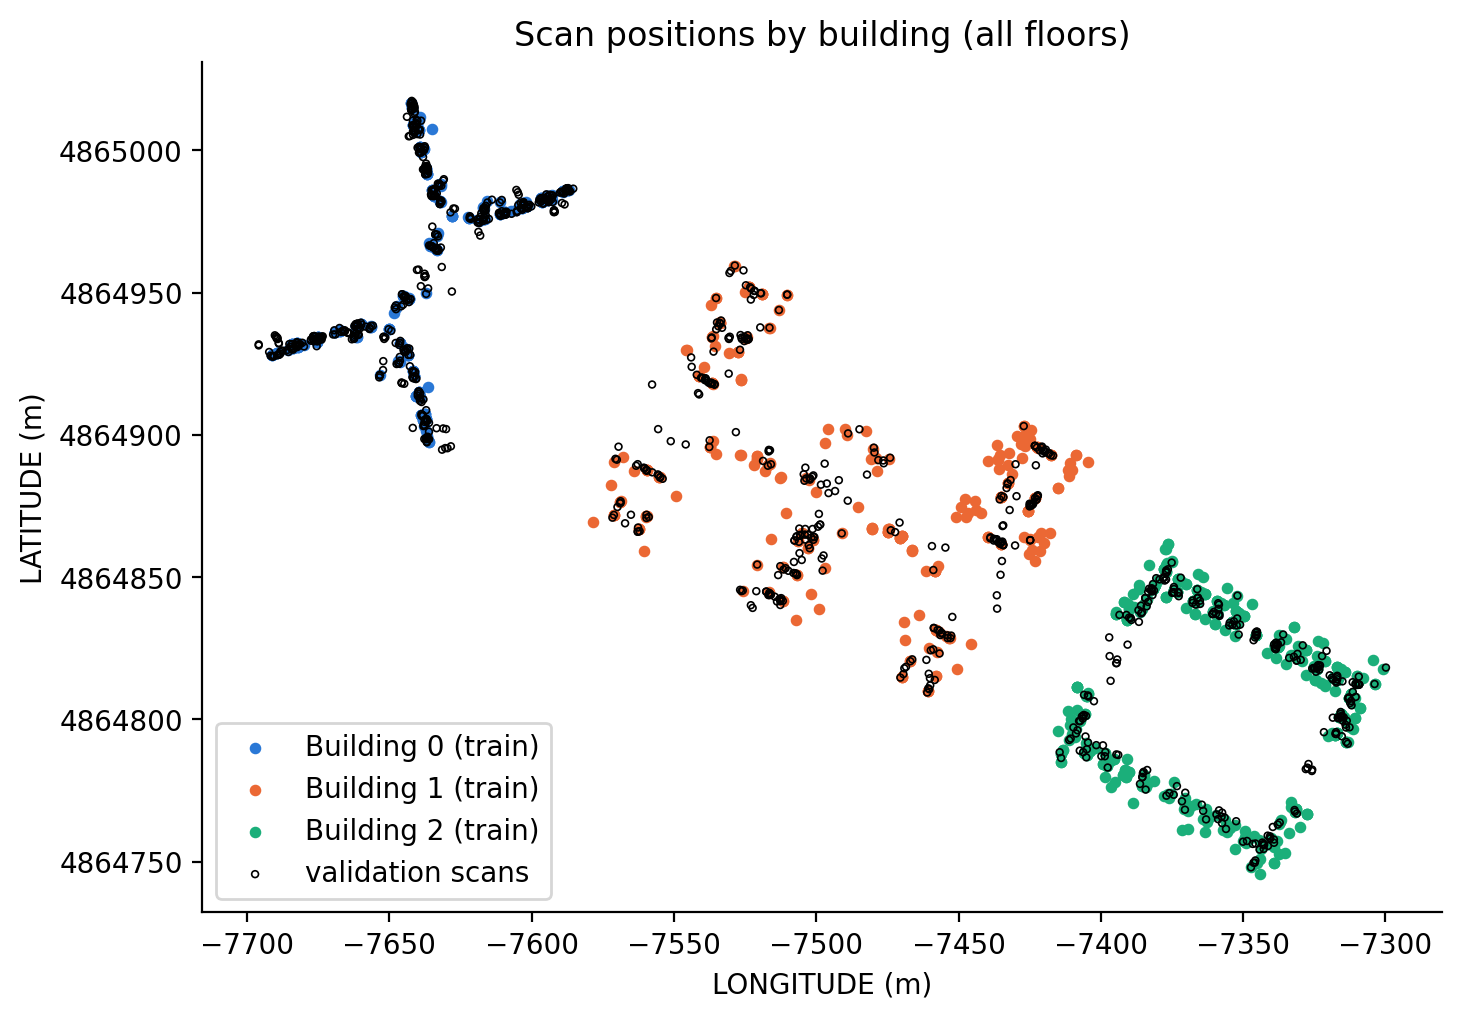
\includegraphics[width=\columnwidth]{eda_map_by_building.png}
\caption{Scan positions in the training file, coloured by building, with validation scans shown as
black circles. The three buildings occupy separate areas of the campus.}
\label{fig:map}
\end{figure}

\subsection{Data Quality}

Table~\ref{tab:quality} lists the quality checks and their outcome. The data is reliable overall: all
real RSSI values lie in the documented range, the labels are valid (floor~4 exists only in
building~2, the only five-floor building), and the three buildings are spatially separate
(Fig.~\ref{fig:map}).

A few issues require preprocessing decisions. First, 76 training scans detected no access point at all
and therefore carry no information; 59 of them come from a single user and phone, which points to a
faulty recording session. Second, there are 637 exact duplicate rows (3.2\% of the training file); none
of them has conflicting labels, but duplicates can inflate validation scores if copies fall on both sides
of a split. Third, 55 access points are never detected in the training file, so their columns are
constant and can be removed. The same 55 access points do appear in the validation file, while 153
access points seen in training never appear in validation, which shows that the Wi-Fi infrastructure
changed between the two collections.

Finally, 775 readings stronger than $-30$~dBm occur in 492 training scans, whereas the strongest
validation reading is $-34$~dBm. 87\% of these scans come from one device (phone~19), so we treat them
as a device artefact; capping readings at $-30$~dBm removes them.

\begin{table}[!t]
\centering
\caption{Data-quality checks on the training file}
\label{tab:quality}
\setlength{\tabcolsep}{3pt}
\begin{tabular}{p{0.27\columnwidth}p{0.40\columnwidth}p{0.27\columnwidth}}
\toprule
\textbf{Check} & \textbf{Result} & \textbf{Action} \\
\midrule
RSSI range & All real values in $[-104, 0]$ & None \\
Labels & Valid; floor 4 only in building 2 & None \\
Empty scans & 76 (59 from one device) & Remove \\
Duplicates & 637 exact duplicates & Remove before splitting \\
Never-detected APs & 55 constant columns & Drop \\
Very strong readings & 492 scans, 87\% from phone 19 & Cap at $-30$ dBm \\
Validation metadata & User, room and position columns are always 0 & Never use as inputs \\
\bottomrule
\end{tabular}
\end{table}

\subsection{Label Distributions}

Fig.~\ref{fig:buildings} shows that the two files emphasise different buildings: building~2 makes up
47.6\% of the training scans, while building~0 makes up 48.2\% of the validation scans. Overall
validation accuracy is therefore driven mostly by building~0, and we report results per building as
well as overall.

Class imbalance is moderate (Fig.~\ref{fig:classes}). Every building--floor combination has at least
948 training scans, recorded at 50--113 distinct positions with about 20 scans per position. The
largest combination (building~2, floor~3) has 2.9 times as many scans as the smallest (building~1,
floor~3). A classifier that always predicts the most frequent class would reach 47.6\% building
accuracy and 25.3\% floor accuracy; these are the baselines any model must clearly exceed. Because of
the imbalance, we report macro-F1 alongside accuracy.

\begin{figure}[!t]
\centering
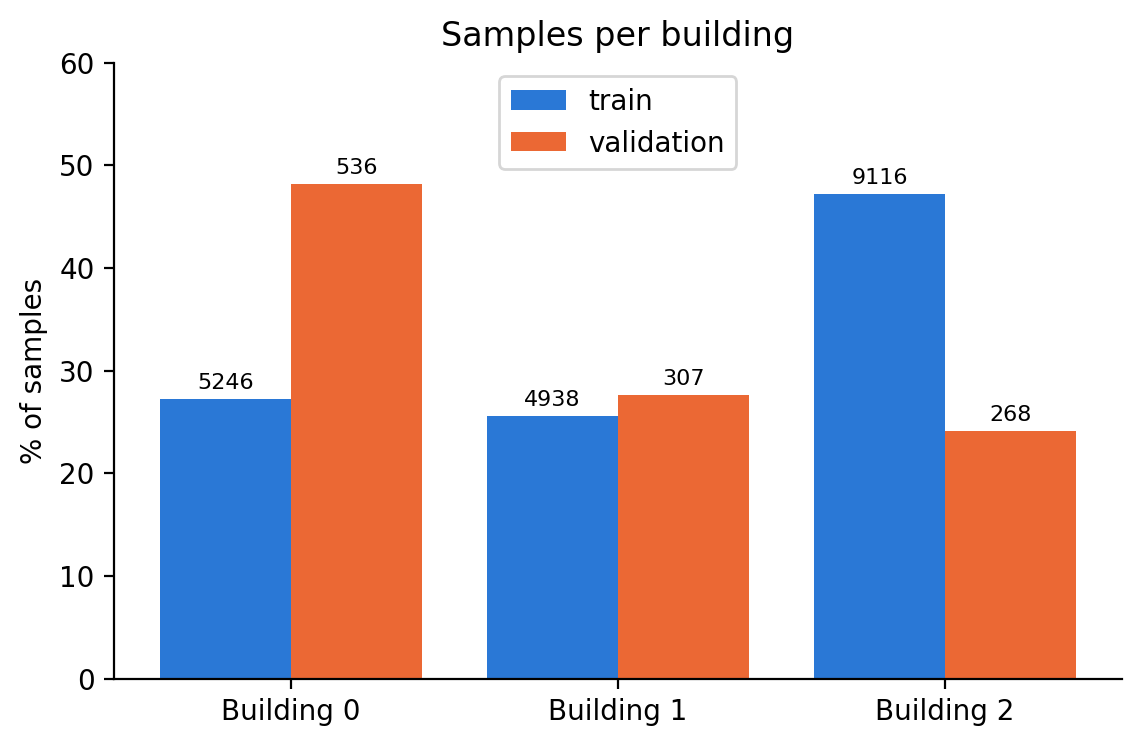
\includegraphics[width=0.9\columnwidth]{eda_samples_per_building.png}
\caption{Share of scans per building in each file (counts above the bars).}
\label{fig:buildings}
\end{figure}

\begin{figure}[!t]
\centering
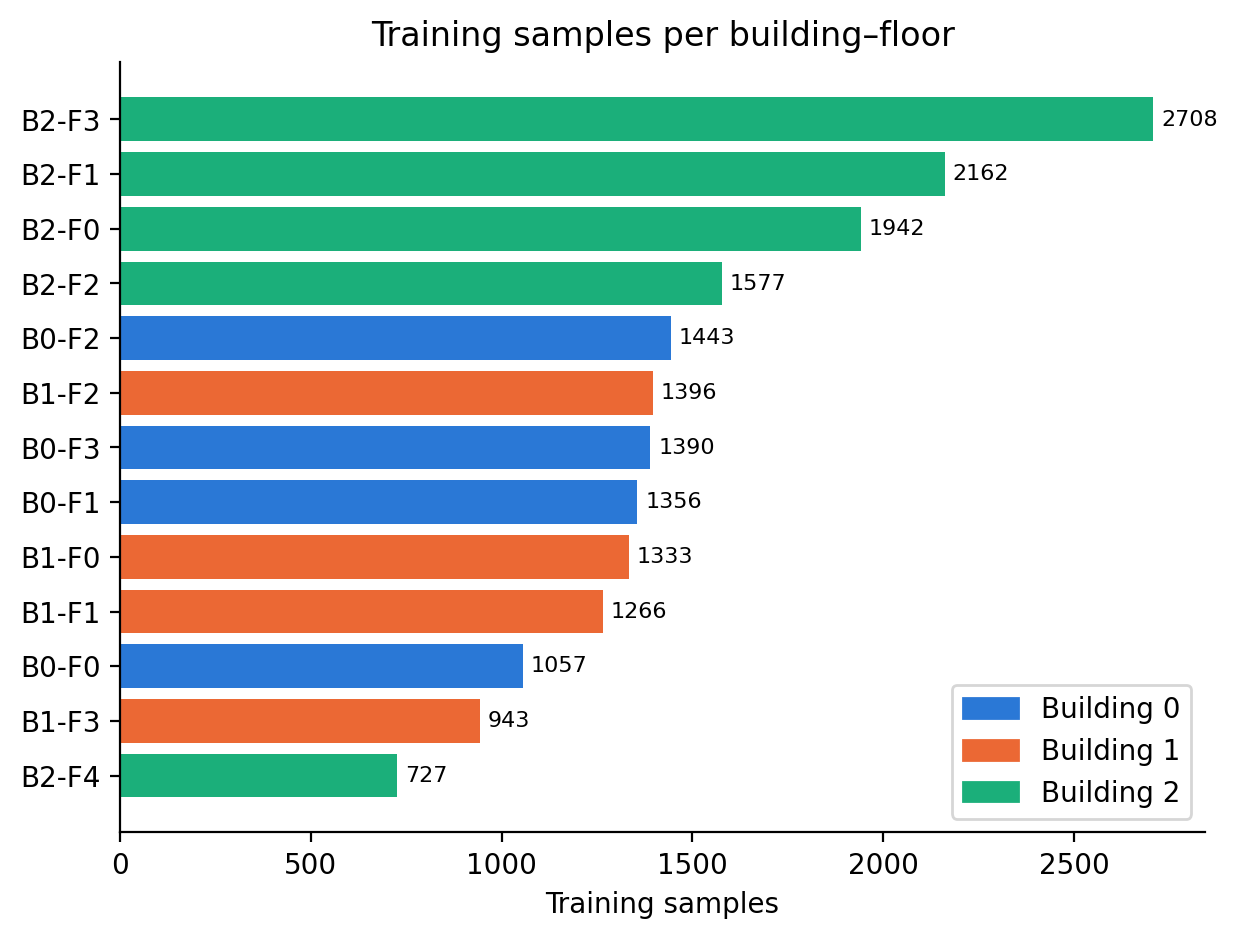
\includegraphics[width=0.9\columnwidth]{eda_building_floor_classes.png}
\caption{Training scans for each of the 13 building--floor combinations.}
\label{fig:classes}
\end{figure}

\subsection{Signal Characteristics}

The data is extremely sparse: 96.5\% of all signal values are ``not detected'', and a typical scan
picks up only 17 of the 520 access points. Among the real readings, most signals are weak, with a median
of $-82$~dBm in training and $-80$~dBm in validation (Fig.~\ref{fig:rssi}). Since the weakest real
reading is $-104$~dBm, the placeholder $+100$ should be replaced by a lower value such as $-110$~dBm,
which keeps the natural order ``not detected'' $<$ ``weakest detected''.

The number of detected access points also carries location information: scans in building~2 detect a
median of 19 access points, compared with 15--16 in buildings~0 and~1. This motivates aggregate
features for our models (number of detected access points and strongest signal per scan).

\begin{figure}[!t]
\centering
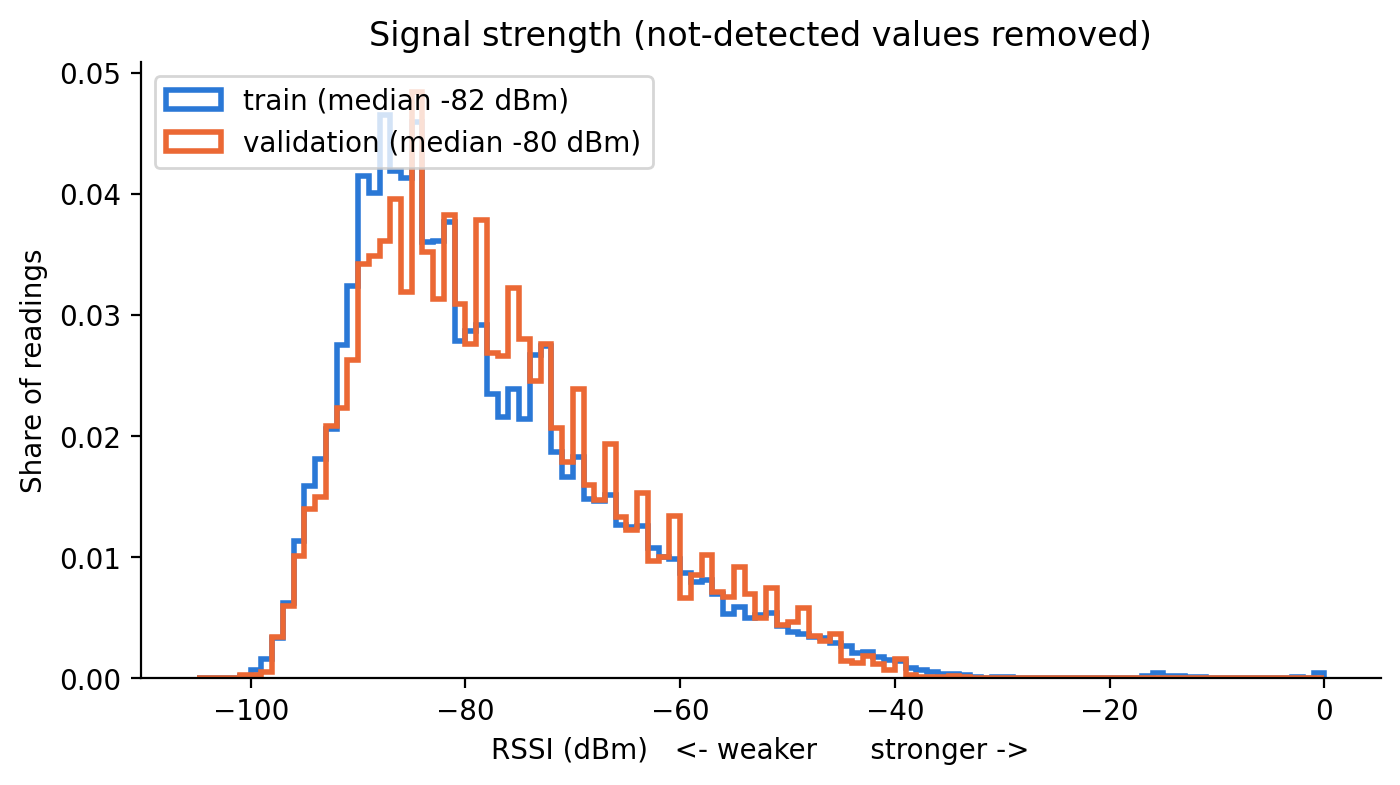
\includegraphics[width=\columnwidth]{eda_rssi_distribution.png}
\caption{Distribution of real RSSI readings (placeholder values removed).}
\label{fig:rssi}
\end{figure}

\subsection{Differences Between the Training and Validation Files}

The two files differ in several ways, so lower scores on the validation file than within the training
file are expected:
\begin{itemize}
\item \textbf{Time:} the files were collected 91 days apart, and each is dominated by a single session
(73.7\% of training scans on one day, 63\% of validation scans on another).
\item \textbf{Phones:} only 2 of the 11 phones in the validation file were used in training. Phones
differ by about 15~dB in typical reported signal strength and detect a median of 9 to 32 access points
per scan (Fig.~\ref{fig:phones}).
\item \textbf{Access points:} the detection rates of individual access points are only moderately
correlated between the files ($r = 0.64$), and 55 access points appear only in validation.
\item \textbf{Signal distributions:} a Kolmogorov--Smirnov test shows a moderate shift in the number of
access points per scan (KS $= 0.13$) and only small shifts in signal strength (KS $= 0.06$--$0.08$).
\end{itemize}

Despite these differences, the validation scans are well covered spatially: the median distance from a
validation scan to the nearest training position on the same floor is 0.9~m, and 90\% are within 4.6~m.
However, 35 validation scans (3.2\%) are more than 10~m from any training position, and we expect the
largest positioning errors there.

\begin{figure*}[!t]
\centering
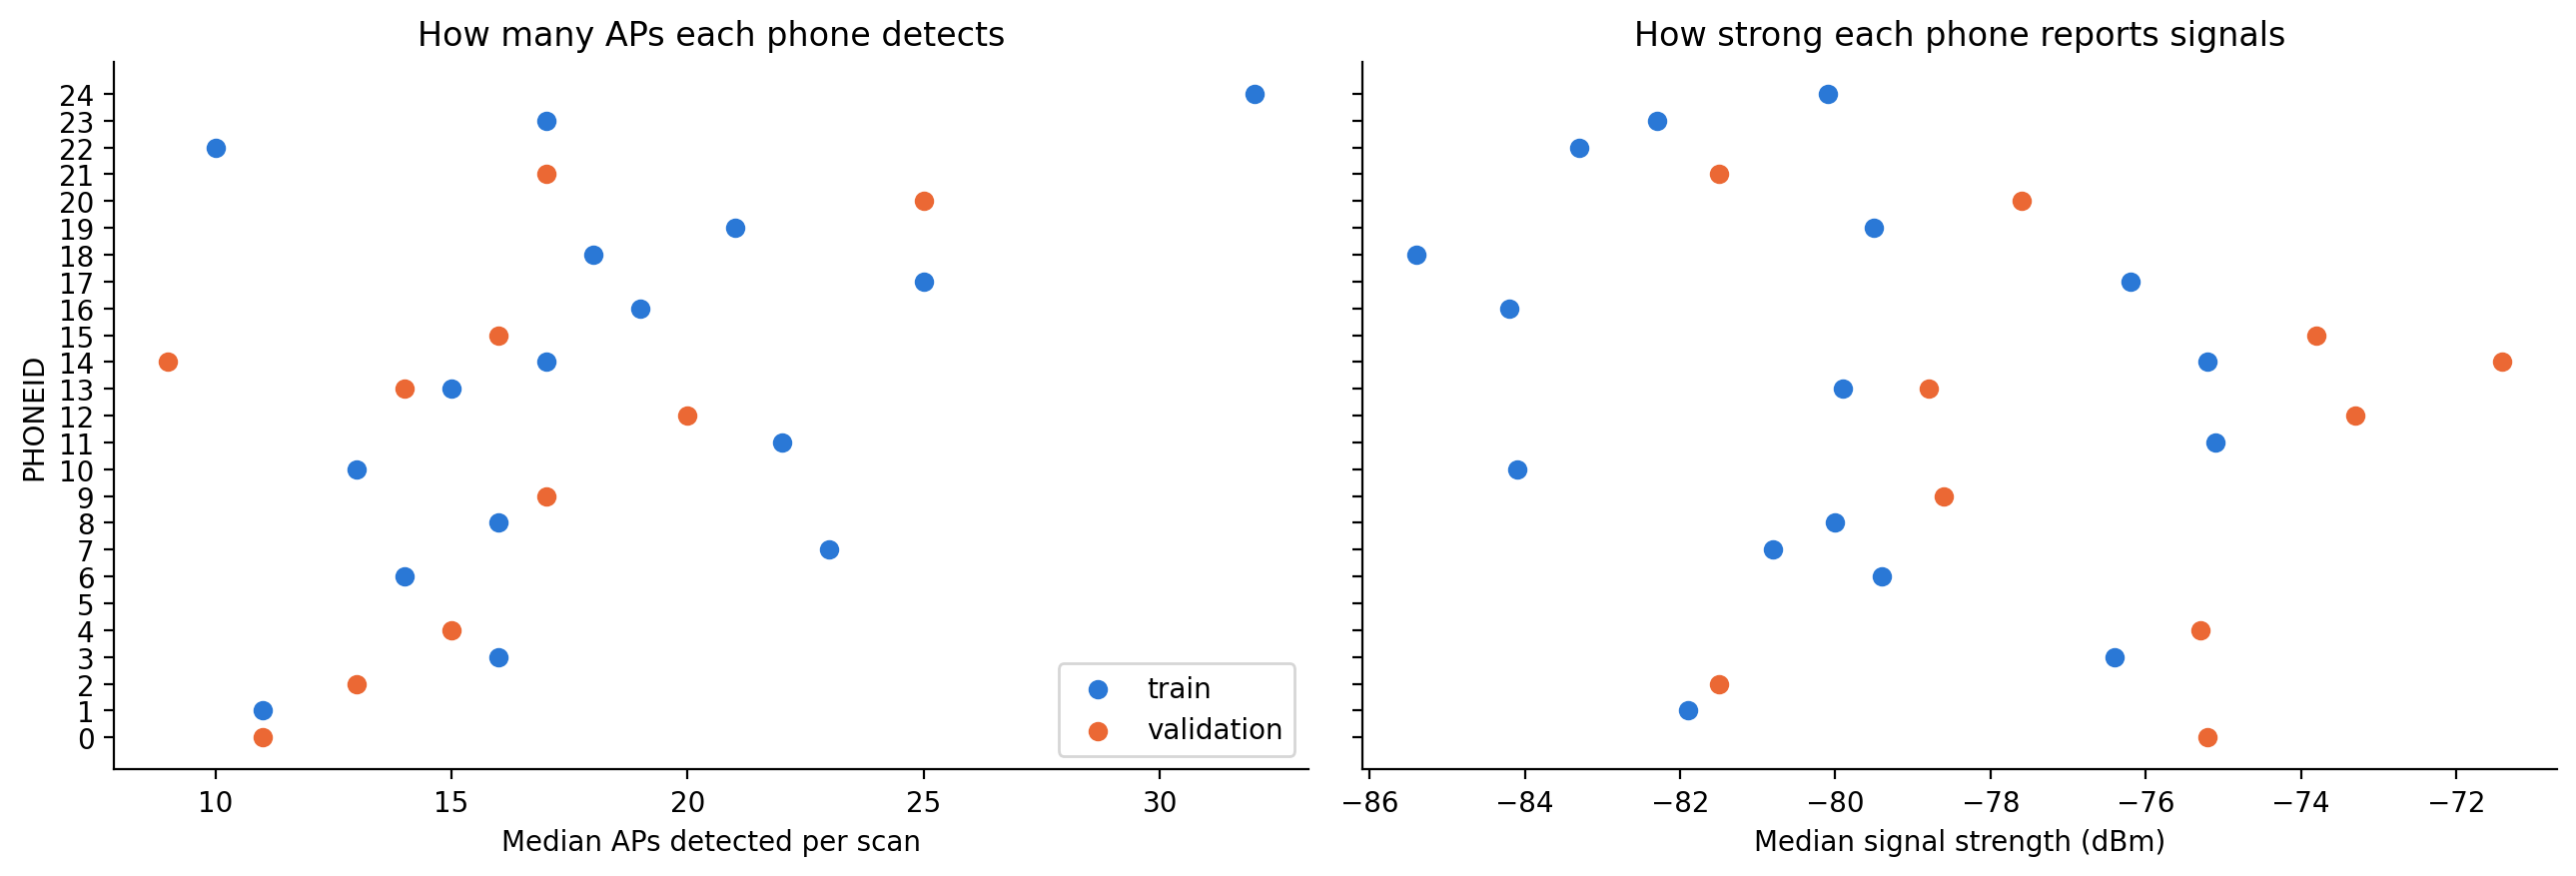
\includegraphics[width=0.85\textwidth]{eda_phone_differences.png}
\caption{Differences between phones (phones with at least 20 scans). Left: median number of access
points detected per scan. Right: median signal strength. Most validation phones (orange) were never
used in training.}
\label{fig:phones}
\end{figure*}

\subsection{Leakage Risks and Validation Strategy}

Each training position was scanned about 20 times, and each user collected only 1 to 8 of the 13
building--floor combinations using exactly one phone (Fig.~\ref{fig:users}). These properties determine
how models can be validated fairly. Table~\ref{tab:leakage} shows, for different 5-fold splits of the
training file, the share of test-fold scans whose exact position also appears in the training fold.

\begin{table}[!t]
\centering
\caption{Share of test-fold scans at a position already seen in training (5-fold splits of the training file)}
\label{tab:leakage}
\begin{tabular}{lr}
\toprule
\textbf{Split} & \textbf{Positions already seen} \\
\midrule
Random 5-fold & 100.0\% \\
Grouped by user & 67.3\% \\
Grouped by position & 0.0\% \\
\bottomrule
\end{tabular}
\end{table}

A random split places every test scan at a position the model has already seen, which would give
unrealistically optimistic scores. We therefore adopt the following protocol:
\begin{enumerate}
\item \textbf{Final results:} train on the training file and evaluate once on the validation file. No
validation scan is identical to a training scan, so this split has no direct leakage.
\item \textbf{Hyperparameter tuning:} 5-fold cross-validation within the training file, grouped by
position.
\item \textbf{Robustness:} 5-fold cross-validation grouped by user. Since each user used one phone, this
also tests generalisation to an unseen device.
\end{enumerate}
In addition, all preprocessing steps (placeholder replacement, scaling and column removal) are fitted on
the training file only, and the room-level columns \texttt{SPACEID} and \texttt{RELATIVEPOSITION} are
never used as inputs because they directly encode the location.

\begin{figure}[!t]
\centering
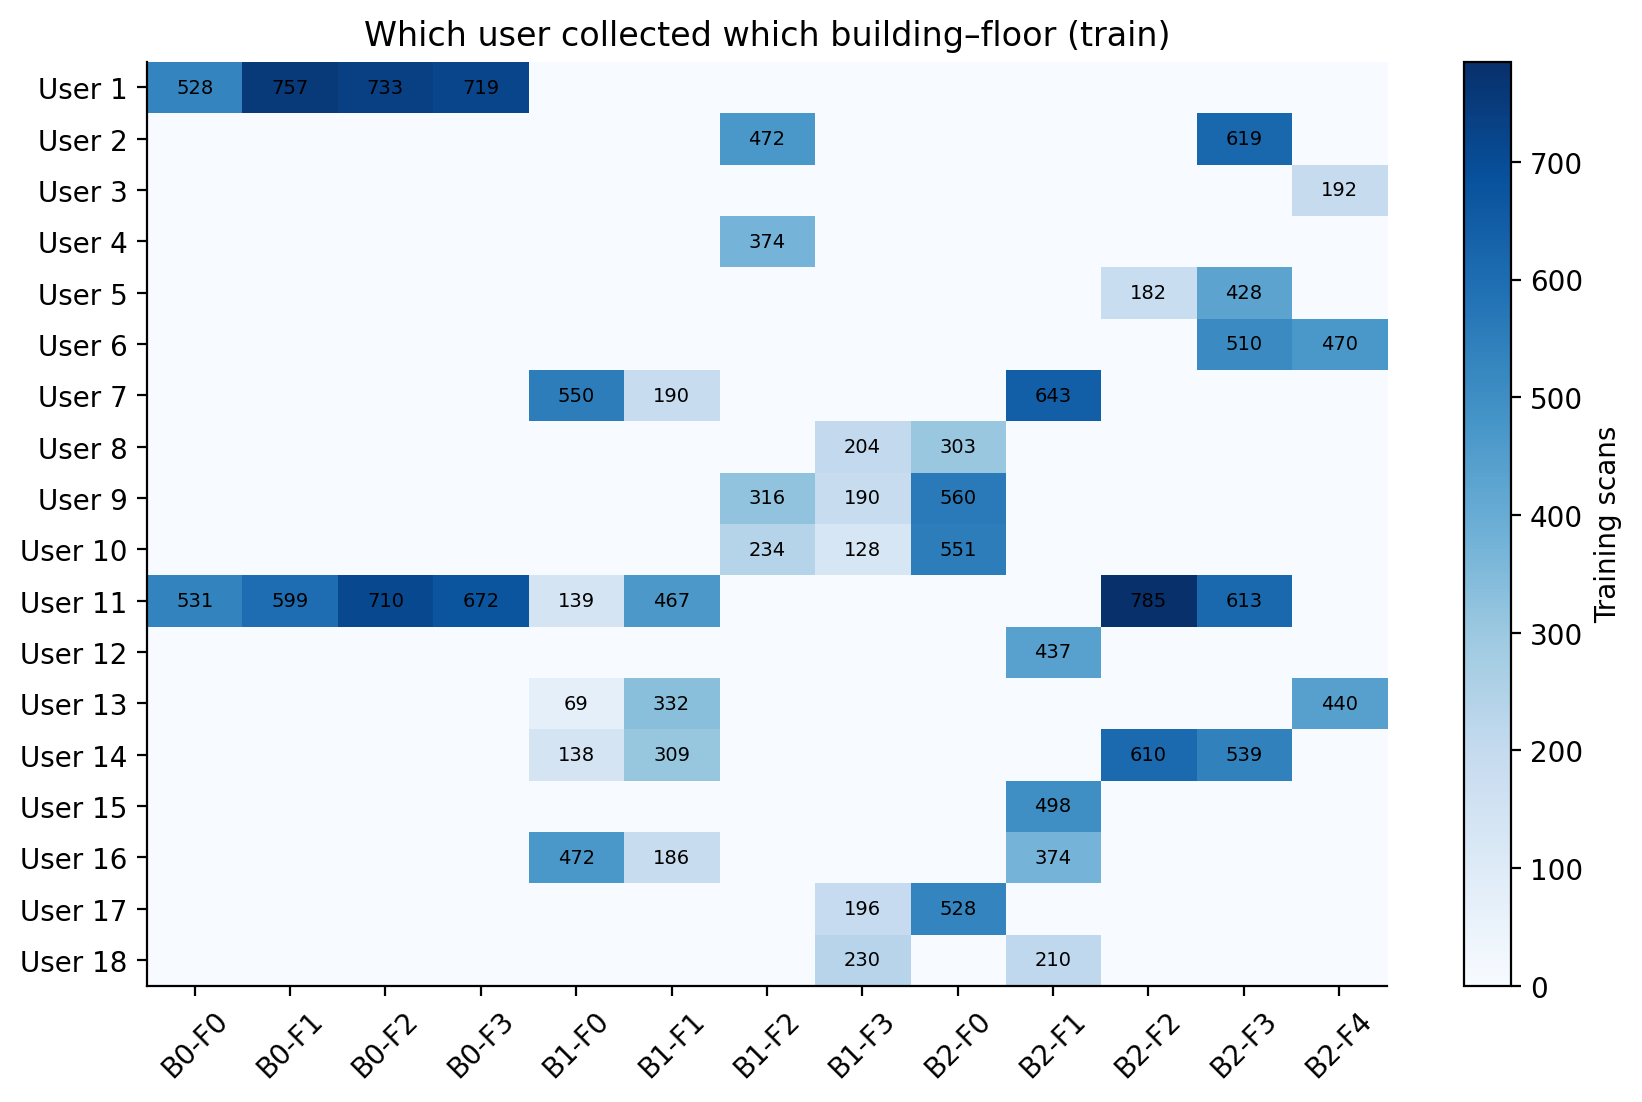
\includegraphics[width=\columnwidth]{eda_user_coverage.png}
\caption{Number of training scans collected by each user in each building--floor combination.}
\label{fig:users}
\end{figure}

% Figures are read from ../results/figures/ (see \graphicspath in main.tex)
% ---------------------------------------------------------------

\subsection{Dataset}

We use the UJIIndoorLoc dataset~\cite{torres2014ujiindoorloc, uci_ujiindoorloc}, a public benchmark for
Wi-Fi fingerprinting collected in three buildings of Universitat Jaume I, Spain. Each row is one Wi-Fi
scan taken by a smartphone. It contains the received signal strength (RSSI) of 520 wireless access
points (WAPs), the true location of the phone, and information about who took the scan, with which
phone, and when.

RSSI values are given in dBm and range from $-104$ (very weak) to $0$ (very strong). An access point
that was not detected is recorded as $+100$. This value is a placeholder, not a measurement, and it
must be handled explicitly because otherwise it would look like the strongest possible signal.

The prediction targets are the building (3 classes) and floor (5 classes), treated as classification,
and the longitude and latitude, treated as regression. The coordinates are projected positions in
metres, so positioning error can be reported in metres. The remaining columns (\texttt{SPACEID},
\texttt{RELATIVEPOSITION}, \texttt{USERID}, \texttt{PHONEID}, \texttt{TIMESTAMP}) are not used as model
inputs; we use them only for quality checks and to design fair validation splits.

The dataset is provided as two files: a training file and a validation file. The labels of the original
competition test set were never released, so, following common practice, we use the validation file
as our held-out test set and do not use it for any modelling decision. Table~\ref{tab:summary}
summarises both files.

\begin{table}[!t]
\centering
\caption{Summary of the two data files}
\label{tab:summary}
\begin{tabular}{lrr}
\toprule
 & \textbf{Train} & \textbf{Validation} \\
\midrule
Scans (rows) & 19{,}937 & 1{,}111 \\
Buildings / floors & 3 / 5 & 3 / 5 \\
Building--floor combinations & 13 & 13 \\
Users / phones & 18 / 16 & -- / 11 \\
Collection period & May--Jun 2013 & Sep--Oct 2013 \\
Signal values $=100$ (not detected) & 96.5\% & 96.8\% \\
Median APs detected per scan & 17 & 15 \\
Scans with no AP detected & 76 & 0 \\
Exact duplicate rows & 637 & 0 \\
\bottomrule
\end{tabular}
\end{table}

\begin{figure}[!t]
\centering
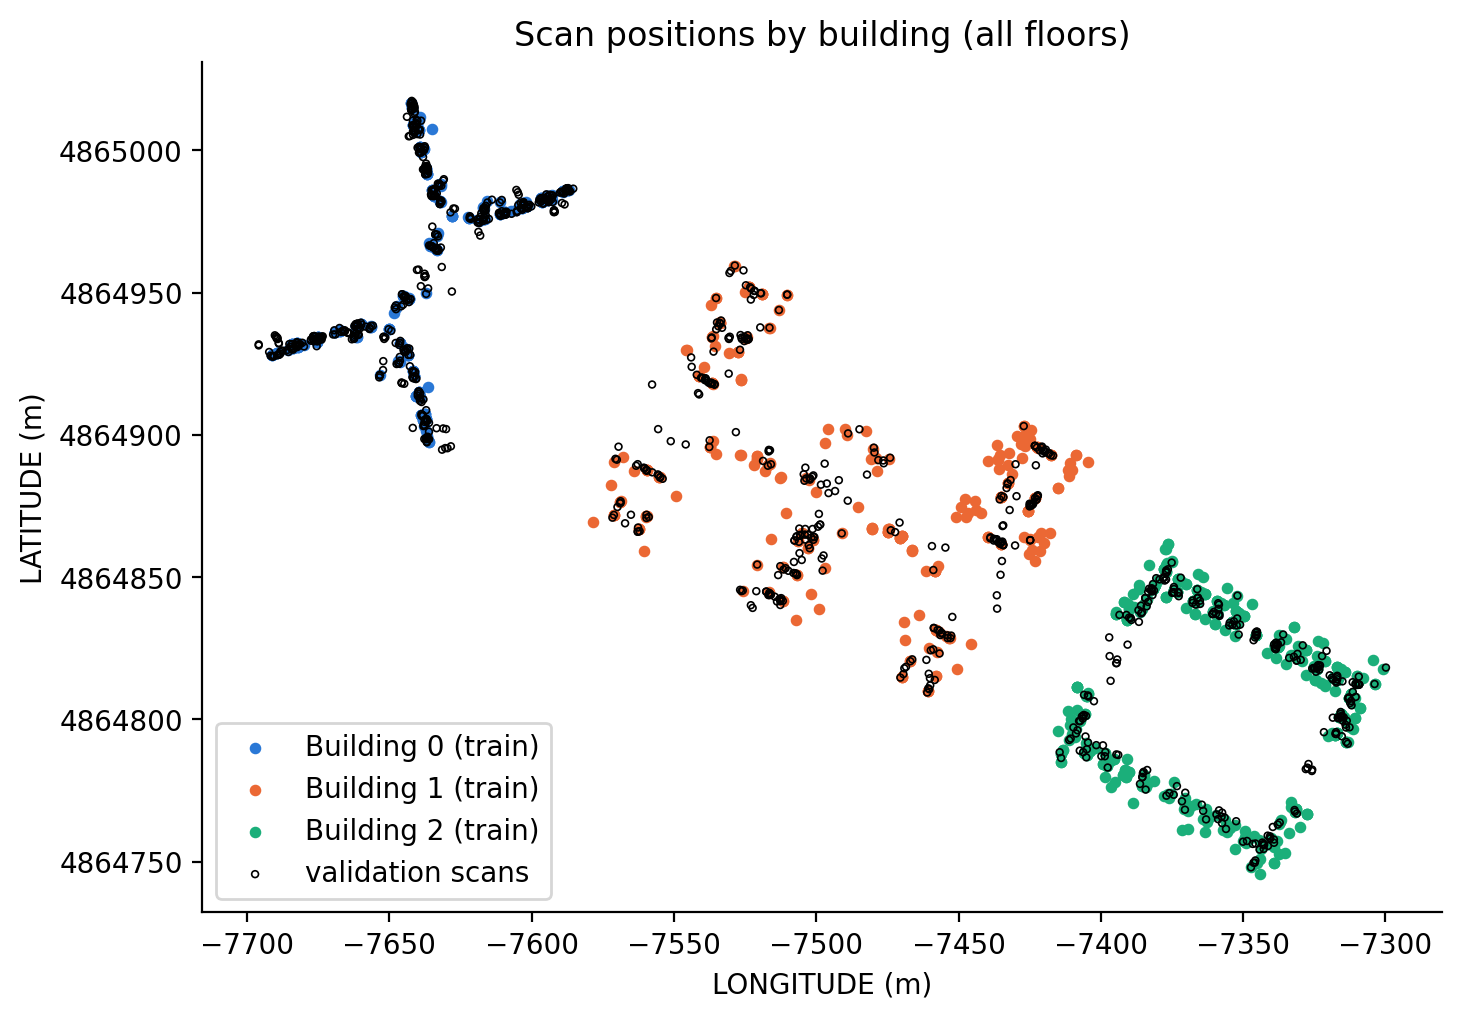
\includegraphics[width=\columnwidth]{eda_map_by_building.png}
\caption{Scan positions in the training file, coloured by building, with validation scans shown as
black circles. The three buildings occupy separate areas of the campus.}
\label{fig:map}
\end{figure}

\subsection{Data Quality}

Table~\ref{tab:quality} lists the quality checks and their outcome. The data is reliable overall: all
real RSSI values lie in the documented range, the labels are valid (floor~4 exists only in
building~2, the only five-floor building), and the three buildings are spatially separate
(Fig.~\ref{fig:map}).

A few issues require preprocessing decisions. First, 76 training scans detected no access point at all
and therefore carry no information; 59 of them come from a single user and phone, which points to a
faulty recording session. Second, there are 637 exact duplicate rows (3.2\% of the training file); none
of them has conflicting labels, but duplicates can inflate validation scores if copies fall on both sides
of a split. Third, 55 access points are never detected in the training file, so their columns are
constant and can be removed. The same 55 access points do appear in the validation file, while 153
access points seen in training never appear in validation, which shows that the Wi-Fi infrastructure
changed between the two collections.

Finally, 775 readings stronger than $-30$~dBm occur in 492 training scans, whereas the strongest
validation reading is $-34$~dBm. 87\% of these scans come from one device (phone~19), so we treat them
as a device artefact; capping readings at $-30$~dBm removes them.

\begin{table}[!t]
\centering
\caption{Data-quality checks on the training file}
\label{tab:quality}
\setlength{\tabcolsep}{3pt}
\begin{tabular}{p{0.27\columnwidth}p{0.40\columnwidth}p{0.27\columnwidth}}
\toprule
\textbf{Check} & \textbf{Result} & \textbf{Action} \\
\midrule
RSSI range & All real values in $[-104, 0]$ & None \\
Labels & Valid; floor 4 only in building 2 & None \\
Empty scans & 76 (59 from one device) & Remove \\
Duplicates & 637 exact duplicates & Remove before splitting \\
Never-detected APs & 55 constant columns & Drop \\
Very strong readings & 492 scans, 87\% from phone 19 & Cap at $-30$ dBm \\
Validation metadata & User, room and position columns are always 0 & Never use as inputs \\
\bottomrule
\end{tabular}
\end{table}

\subsection{Label Distributions}

Fig.~\ref{fig:buildings} shows that the two files emphasise different buildings: building~2 makes up
47.6\% of the training scans, while building~0 makes up 48.2\% of the validation scans. Overall
validation accuracy is therefore driven mostly by building~0, and we report results per building as
well as overall.

Class imbalance is moderate (Fig.~\ref{fig:classes}). Every building--floor combination has at least
948 training scans, recorded at 50--113 distinct positions with about 20 scans per position. The
largest combination (building~2, floor~3) has 2.9 times as many scans as the smallest (building~1,
floor~3). A classifier that always predicts the most frequent class would reach 47.6\% building
accuracy and 25.3\% floor accuracy; these are the baselines any model must clearly exceed. Because of
the imbalance, we report macro-F1 alongside accuracy.

\begin{figure}[!t]
\centering
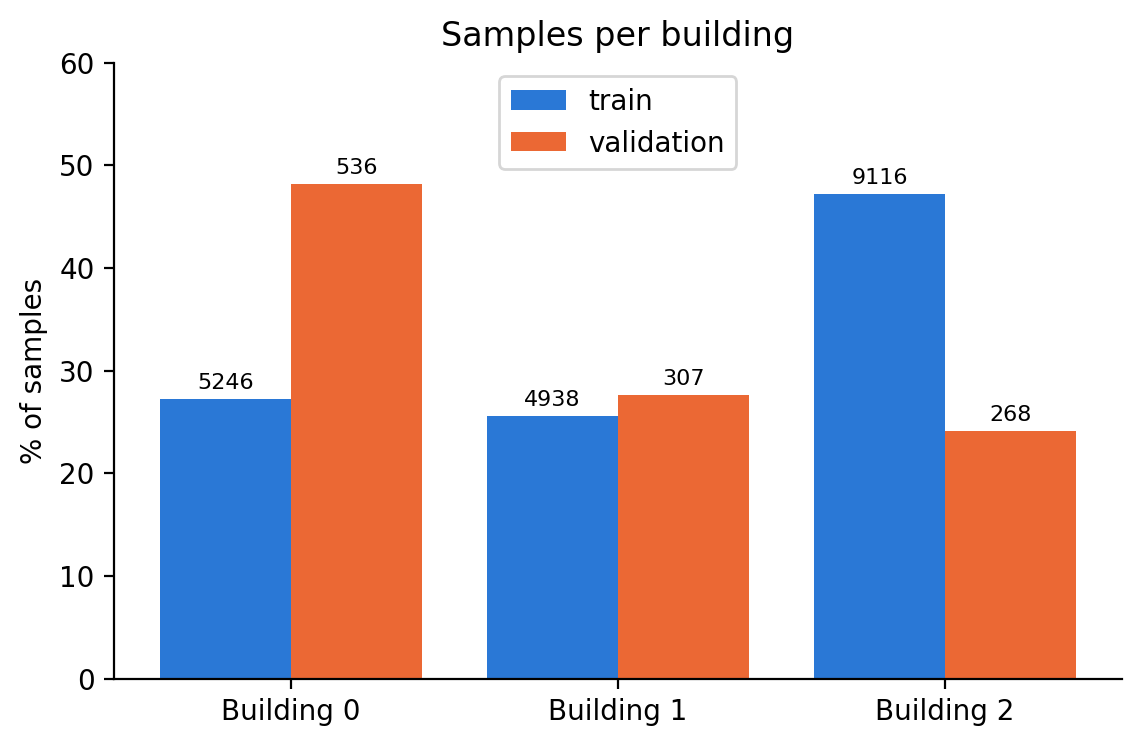
\includegraphics[width=0.9\columnwidth]{eda_samples_per_building.png}
\caption{Share of scans per building in each file (counts above the bars).}
\label{fig:buildings}
\end{figure}

\begin{figure}[!t]
\centering
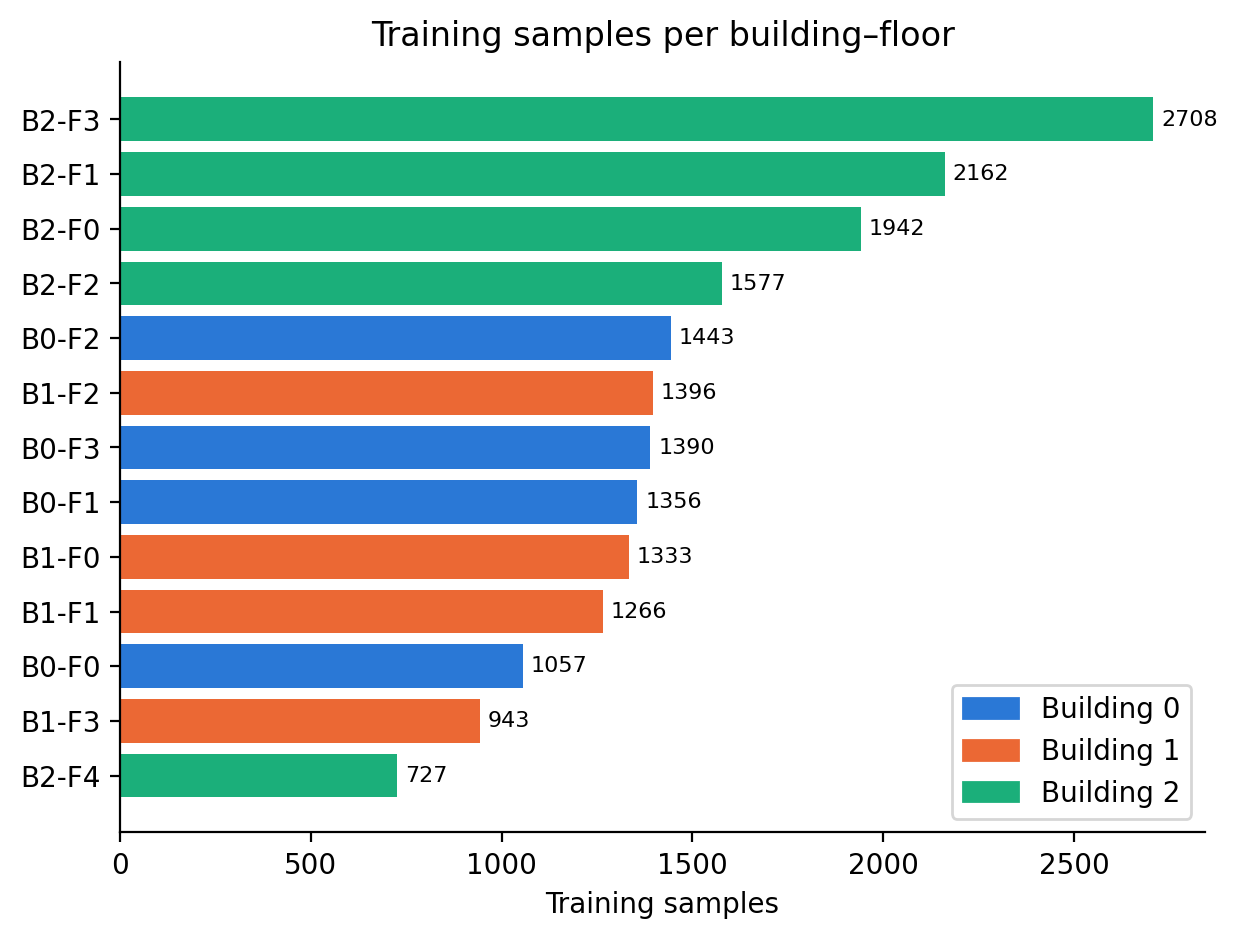
\includegraphics[width=0.9\columnwidth]{eda_building_floor_classes.png}
\caption{Training scans for each of the 13 building--floor combinations.}
\label{fig:classes}
\end{figure}

\subsection{Signal Characteristics}

The data is extremely sparse: 96.5\% of all signal values are ``not detected'', and a typical scan
picks up only 17 of the 520 access points. Among the real readings, most signals are weak, with a median
of $-82$~dBm in training and $-80$~dBm in validation (Fig.~\ref{fig:rssi}). Since the weakest real
reading is $-104$~dBm, the placeholder $+100$ should be replaced by a lower value such as $-110$~dBm,
which keeps the natural order ``not detected'' $<$ ``weakest detected''.

The number of detected access points also carries location information: scans in building~2 detect a
median of 19 access points, compared with 15--16 in buildings~0 and~1. This motivates aggregate
features for our models (number of detected access points and strongest signal per scan).

\begin{figure}[!t]
\centering
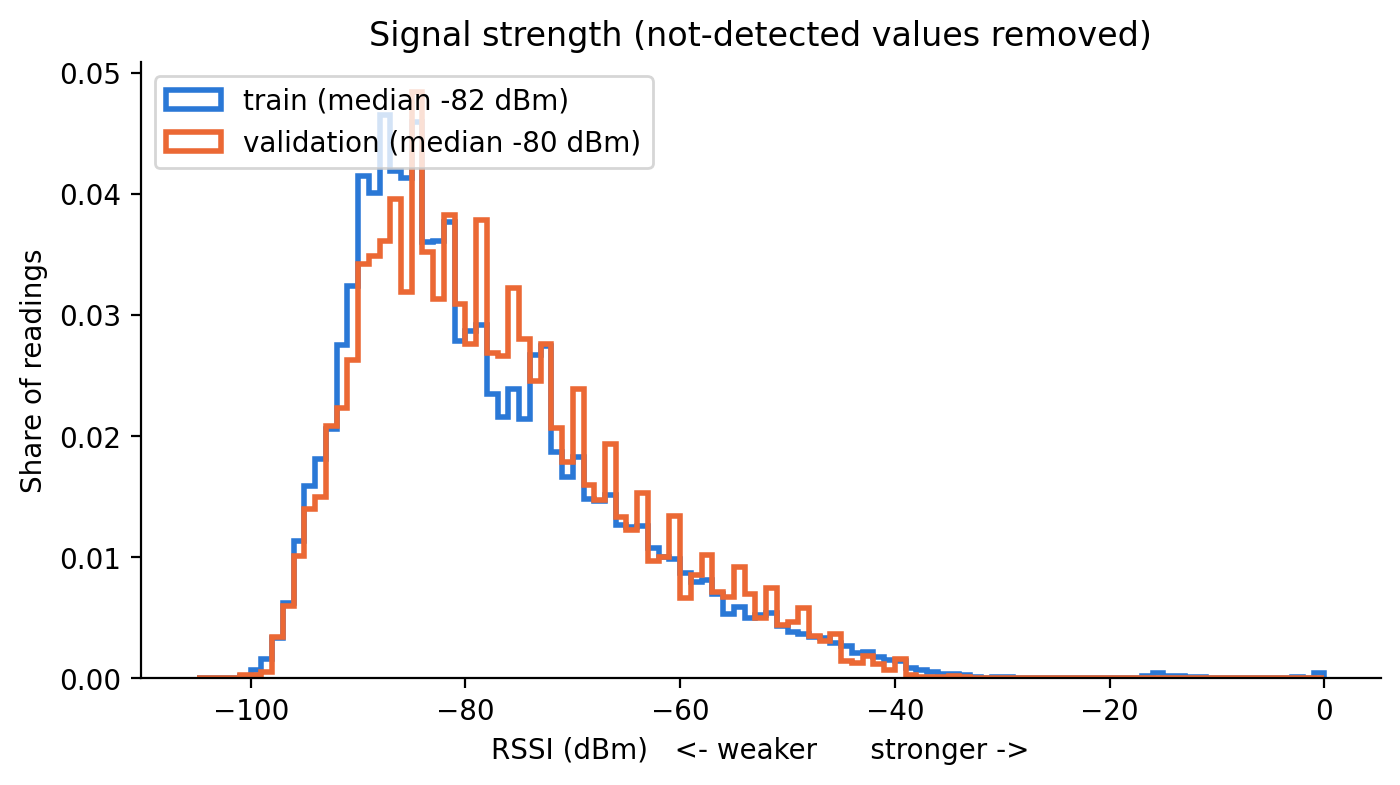
\includegraphics[width=\columnwidth]{eda_rssi_distribution.png}
\caption{Distribution of real RSSI readings (placeholder values removed).}
\label{fig:rssi}
\end{figure}

\subsection{Differences Between the Training and Validation Files}

The two files differ in several ways, so lower scores on the validation file than within the training
file are expected:
\begin{itemize}
\item \textbf{Time:} the files were collected 91 days apart, and each is dominated by a single session
(73.7\% of training scans on one day, 63\% of validation scans on another).
\item \textbf{Phones:} only 2 of the 11 phones in the validation file were used in training. Phones
differ by about 15~dB in typical reported signal strength and detect a median of 9 to 32 access points
per scan (Fig.~\ref{fig:phones}).
\item \textbf{Access points:} the detection rates of individual access points are only moderately
correlated between the files ($r = 0.64$), and 55 access points appear only in validation.
\item \textbf{Signal distributions:} a Kolmogorov--Smirnov test shows a moderate shift in the number of
access points per scan (KS $= 0.13$) and only small shifts in signal strength (KS $= 0.06$--$0.08$).
\end{itemize}

Despite these differences, the validation scans are well covered spatially: the median distance from a
validation scan to the nearest training position on the same floor is 0.9~m, and 90\% are within 4.6~m.
However, 35 validation scans (3.2\%) are more than 10~m from any training position, and we expect the
largest positioning errors there.

\begin{figure*}[!t]
\centering
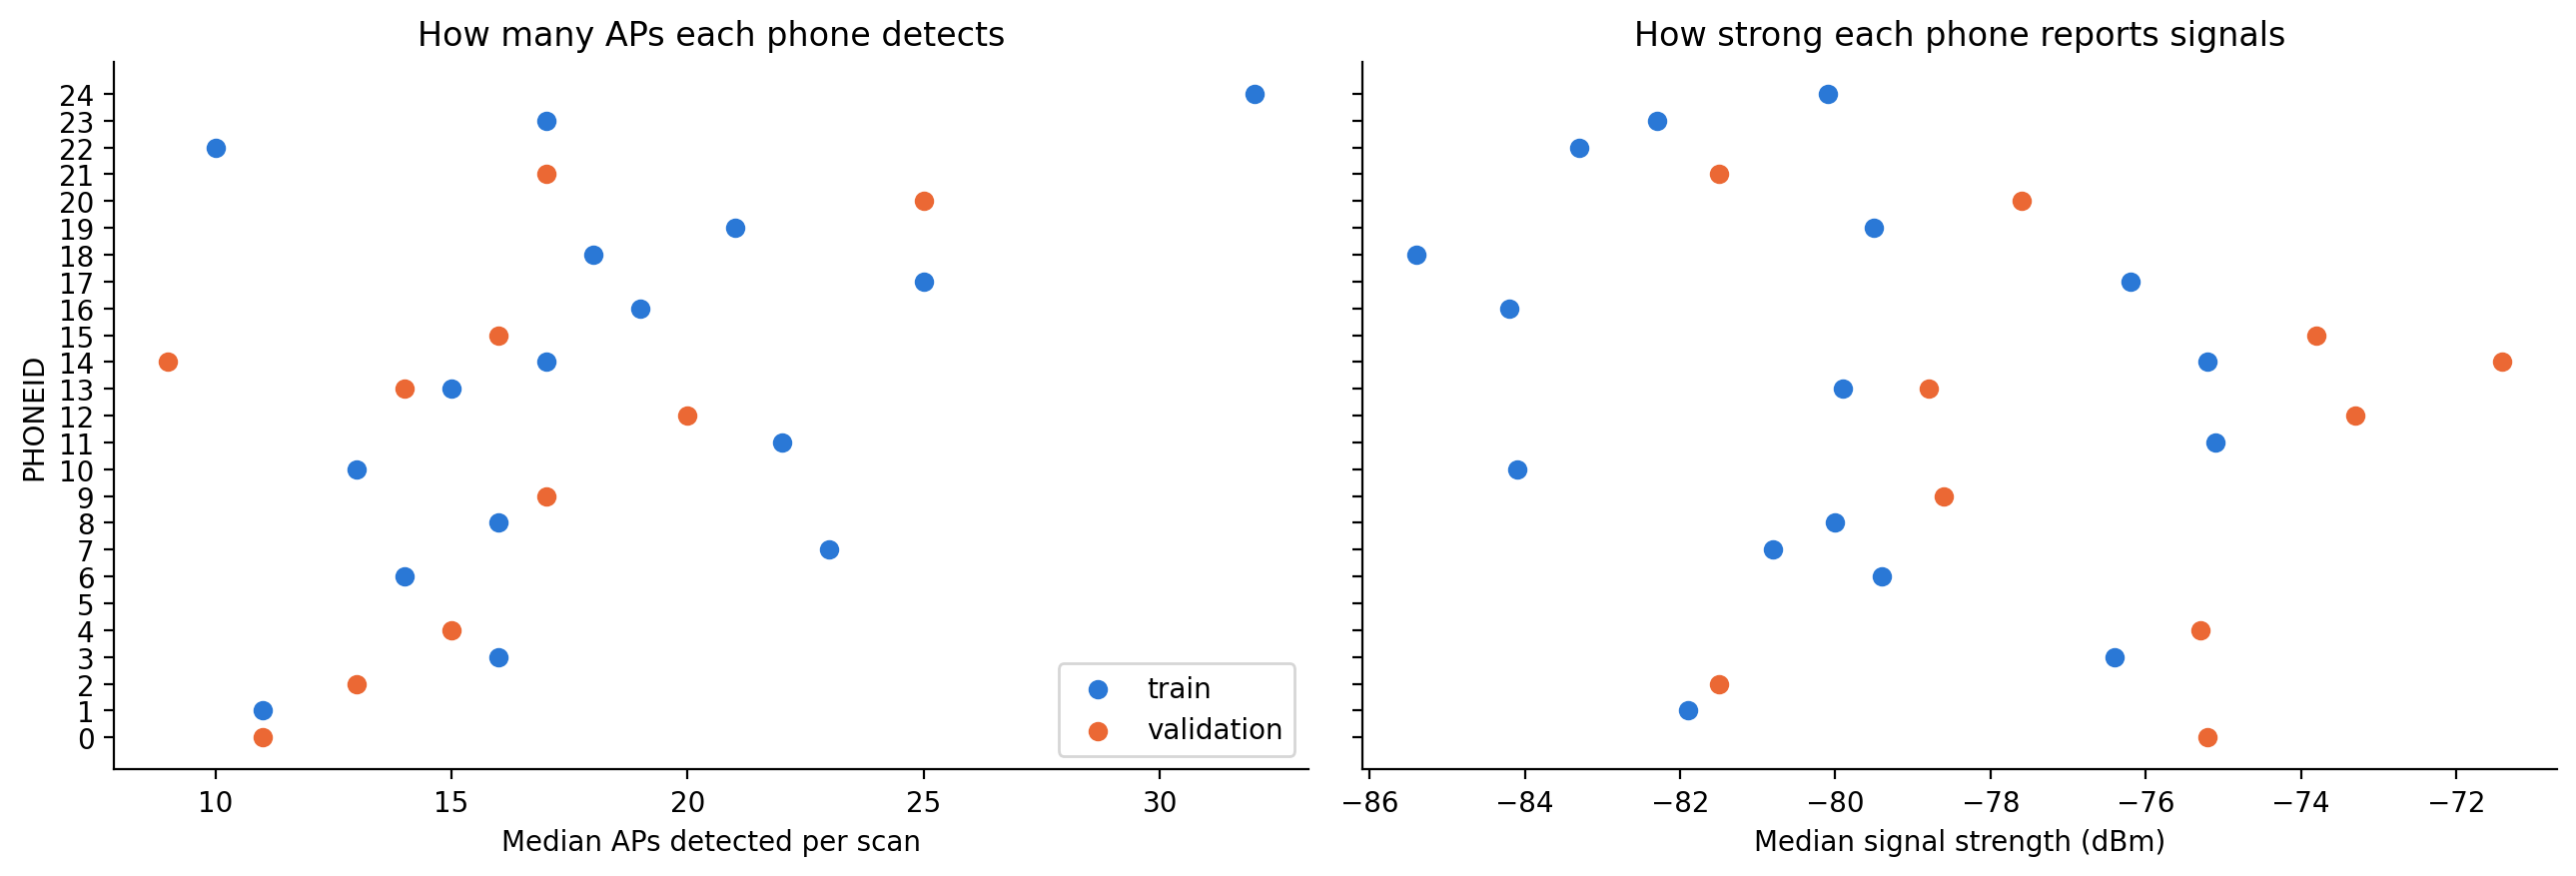
\includegraphics[width=0.85\textwidth]{eda_phone_differences.png}
\caption{Differences between phones (phones with at least 20 scans). Left: median number of access
points detected per scan. Right: median signal strength. Most validation phones (orange) were never
used in training.}
\label{fig:phones}
\end{figure*}

\subsection{Leakage Risks and Validation Strategy}

Each training position was scanned about 20 times, and each user collected only 1 to 8 of the 13
building--floor combinations using exactly one phone (Fig.~\ref{fig:users}). These properties determine
how models can be validated fairly. Table~\ref{tab:leakage} shows, for different 5-fold splits of the
training file, the share of test-fold scans whose exact position also appears in the training fold.

\begin{table}[!t]
\centering
\caption{Share of test-fold scans at a position already seen in training (5-fold splits of the training file)}
\label{tab:leakage}
\begin{tabular}{lr}
\toprule
\textbf{Split} & \textbf{Positions already seen} \\
\midrule
Random 5-fold & 100.0\% \\
Grouped by user & 67.3\% \\
Grouped by position & 0.0\% \\
\bottomrule
\end{tabular}
\end{table}

A random split places every test scan at a position the model has already seen, which would give
unrealistically optimistic scores. We therefore adopt the following protocol:
\begin{enumerate}
\item \textbf{Final results:} train on the training file and evaluate once on the validation file. No
validation scan is identical to a training scan, so this split has no direct leakage.
\item \textbf{Hyperparameter tuning:} 5-fold cross-validation within the training file, grouped by
position.
\item \textbf{Robustness:} 5-fold cross-validation grouped by user. Since each user used one phone, this
also tests generalisation to an unseen device.
\end{enumerate}
In addition, all preprocessing steps (placeholder replacement, scaling and column removal) are fitted on
the training file only, and the room-level columns \texttt{SPACEID} and \texttt{RELATIVEPOSITION} are
never used as inputs because they directly encode the location.

\begin{figure}[!t]
\centering
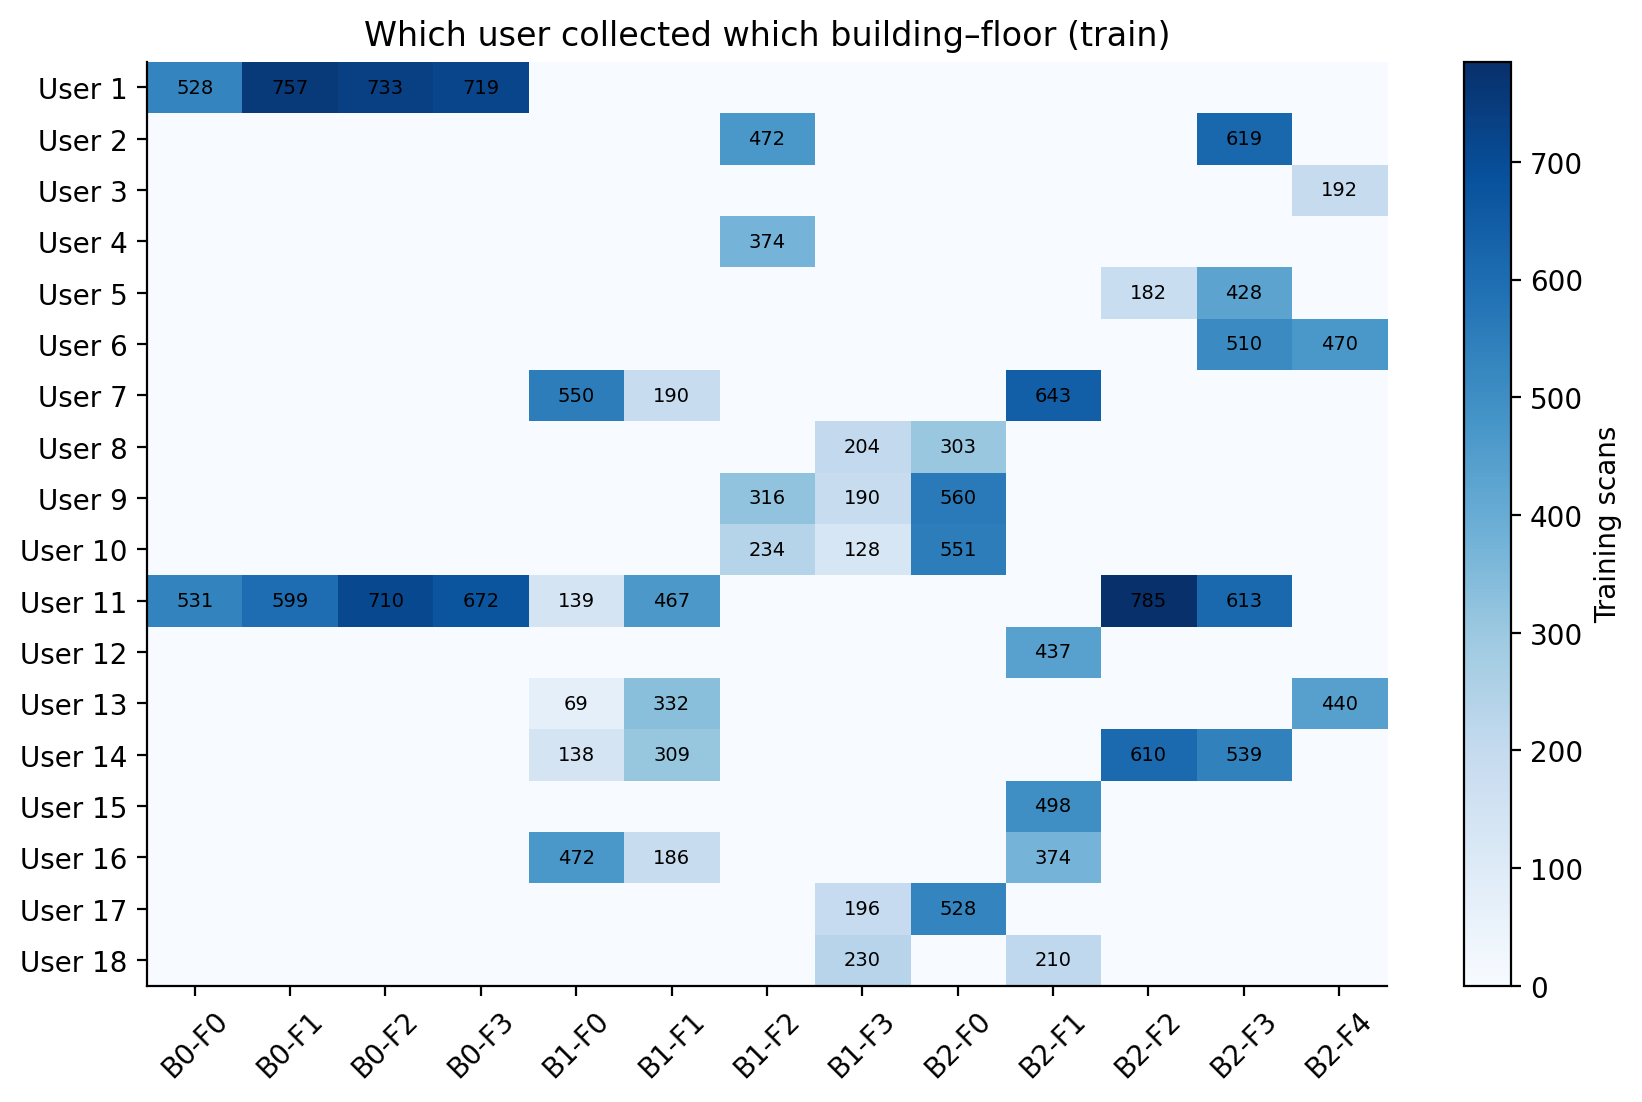
\includegraphics[width=\columnwidth]{eda_user_coverage.png}
\caption{Number of training scans collected by each user in each building--floor combination.}
\label{fig:users}
\end{figure}

% Figures are read from ../results/figures/ (see \graphicspath in main.tex)
% ---------------------------------------------------------------

\subsection{Dataset}

We use the UJIIndoorLoc dataset~\cite{torres2014ujiindoorloc, uci_ujiindoorloc}, a public benchmark for
Wi-Fi fingerprinting collected in three buildings of Universitat Jaume I, Spain. Each row is one Wi-Fi
scan taken by a smartphone. It contains the received signal strength (RSSI) of 520 wireless access
points (WAPs), the true location of the phone, and information about who took the scan, with which
phone, and when.

RSSI values are given in dBm and range from $-104$ (very weak) to $0$ (very strong). An access point
that was not detected is recorded as $+100$. This value is a placeholder, not a measurement, and it
must be handled explicitly because otherwise it would look like the strongest possible signal.

The prediction targets are the building (3 classes) and floor (5 classes), treated as classification,
and the longitude and latitude, treated as regression. The coordinates are projected positions in
metres, so positioning error can be reported in metres. The remaining columns (\texttt{SPACEID},
\texttt{RELATIVEPOSITION}, \texttt{USERID}, \texttt{PHONEID}, \texttt{TIMESTAMP}) are not used as model
inputs; we use them only for quality checks and to design fair validation splits.

The dataset is provided as two files: a training file and a validation file. The labels of the original
competition test set were never released, so, following common practice, we use the validation file
as our held-out test set and do not use it for any modelling decision. Table~\ref{tab:summary}
summarises both files.

\begin{table}[!t]
\centering
\caption{Summary of the two data files}
\label{tab:summary}
\begin{tabular}{lrr}
\toprule
 & \textbf{Train} & \textbf{Validation} \\
\midrule
Scans (rows) & 19{,}937 & 1{,}111 \\
Buildings / floors & 3 / 5 & 3 / 5 \\
Building--floor combinations & 13 & 13 \\
Users / phones & 18 / 16 & -- / 11 \\
Collection period & May--Jun 2013 & Sep--Oct 2013 \\
Signal values $=100$ (not detected) & 96.5\% & 96.8\% \\
Median APs detected per scan & 17 & 15 \\
Scans with no AP detected & 76 & 0 \\
Exact duplicate rows & 637 & 0 \\
\bottomrule
\end{tabular}
\end{table}

\begin{figure}[!t]
\centering
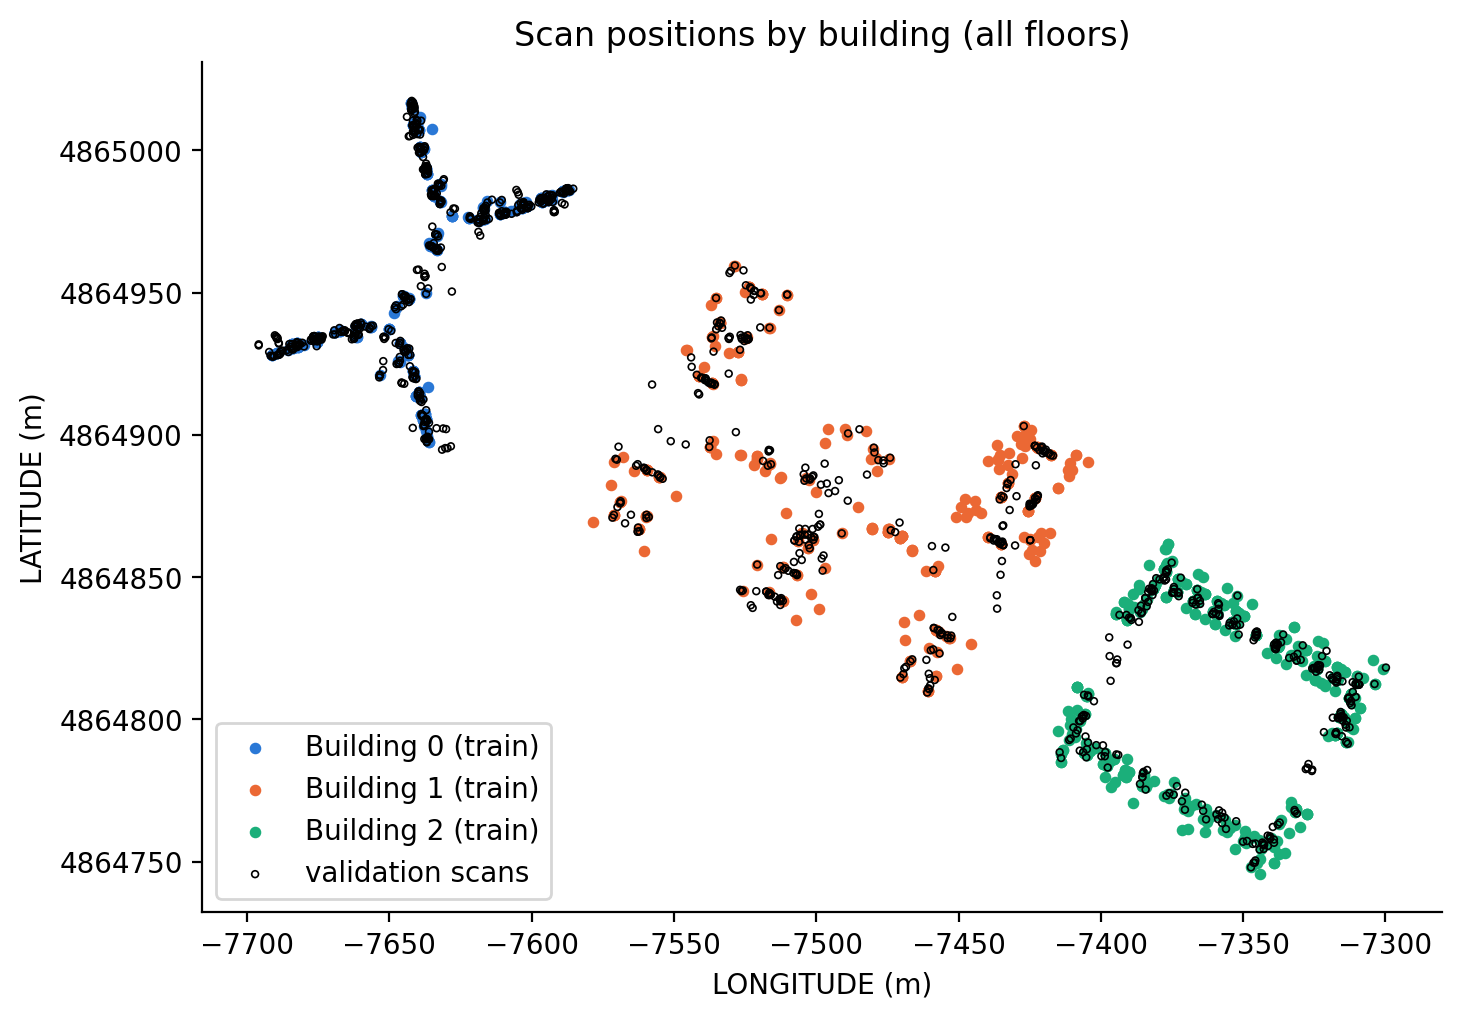
\includegraphics[width=\columnwidth]{eda_map_by_building.png}
\caption{Scan positions in the training file, coloured by building, with validation scans shown as
black circles. The three buildings occupy separate areas of the campus.}
\label{fig:map}
\end{figure}

\subsection{Data Quality}

Table~\ref{tab:quality} lists the quality checks and their outcome. The data is reliable overall: all
real RSSI values lie in the documented range, the labels are valid (floor~4 exists only in
building~2, the only five-floor building), and the three buildings are spatially separate
(Fig.~\ref{fig:map}).

A few issues require preprocessing decisions. First, 76 training scans detected no access point at all
and therefore carry no information; 59 of them come from a single user and phone, which points to a
faulty recording session. Second, there are 637 exact duplicate rows (3.2\% of the training file); none
of them has conflicting labels, but duplicates can inflate validation scores if copies fall on both sides
of a split. Third, 55 access points are never detected in the training file, so their columns are
constant and can be removed. The same 55 access points do appear in the validation file, while 153
access points seen in training never appear in validation, which shows that the Wi-Fi infrastructure
changed between the two collections.

Finally, 775 readings stronger than $-30$~dBm occur in 492 training scans, whereas the strongest
validation reading is $-34$~dBm. 87\% of these scans come from one device (phone~19), so we treat them
as a device artefact; capping readings at $-30$~dBm removes them.

\begin{table}[!t]
\centering
\caption{Data-quality checks on the training file}
\label{tab:quality}
\setlength{\tabcolsep}{3pt}
\begin{tabular}{p{0.27\columnwidth}p{0.40\columnwidth}p{0.27\columnwidth}}
\toprule
\textbf{Check} & \textbf{Result} & \textbf{Action} \\
\midrule
RSSI range & All real values in $[-104, 0]$ & None \\
Labels & Valid; floor 4 only in building 2 & None \\
Empty scans & 76 (59 from one device) & Remove \\
Duplicates & 637 exact duplicates & Remove before splitting \\
Never-detected APs & 55 constant columns & Drop \\
Very strong readings & 492 scans, 87\% from phone 19 & Cap at $-30$ dBm \\
Validation metadata & User, room and position columns are always 0 & Never use as inputs \\
\bottomrule
\end{tabular}
\end{table}

\subsection{Label Distributions}

Fig.~\ref{fig:buildings} shows that the two files emphasise different buildings: building~2 makes up
47.6\% of the training scans, while building~0 makes up 48.2\% of the validation scans. Overall
validation accuracy is therefore driven mostly by building~0, and we report results per building as
well as overall.

Class imbalance is moderate (Fig.~\ref{fig:classes}). Every building--floor combination has at least
948 training scans, recorded at 50--113 distinct positions with about 20 scans per position. The
largest combination (building~2, floor~3) has 2.9 times as many scans as the smallest (building~1,
floor~3). A classifier that always predicts the most frequent class would reach 47.6\% building
accuracy and 25.3\% floor accuracy; these are the baselines any model must clearly exceed. Because of
the imbalance, we report macro-F1 alongside accuracy.

\begin{figure}[!t]
\centering
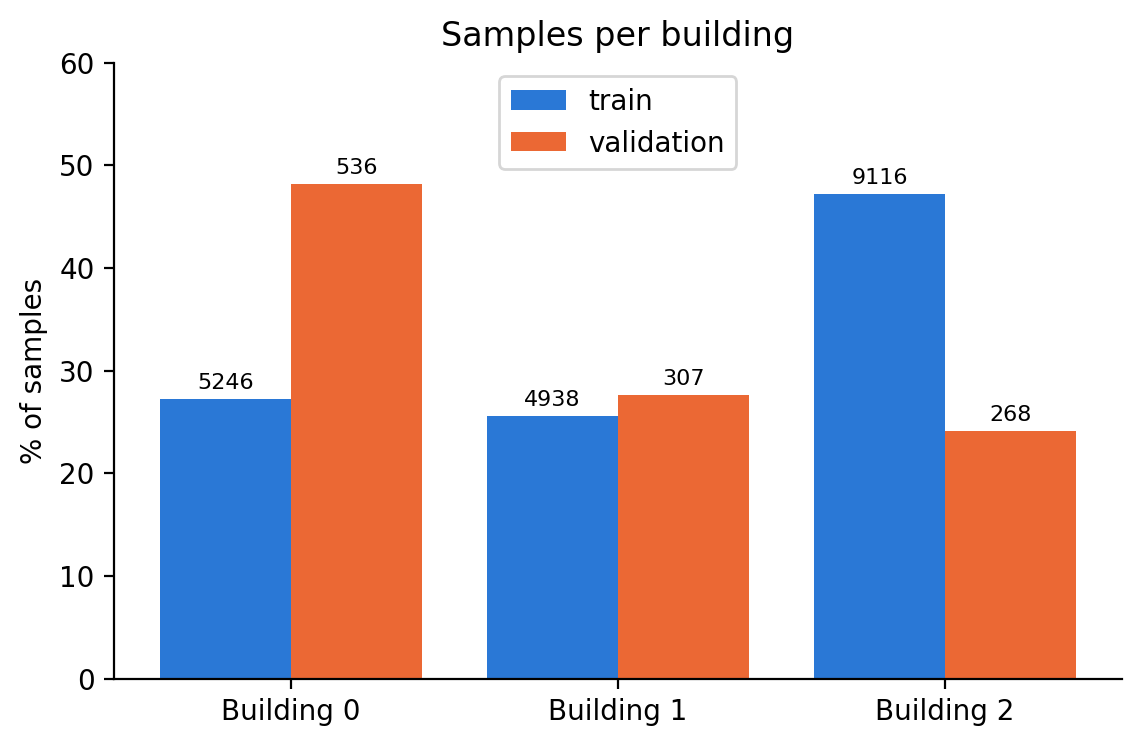
\includegraphics[width=0.9\columnwidth]{eda_samples_per_building.png}
\caption{Share of scans per building in each file (counts above the bars).}
\label{fig:buildings}
\end{figure}

\begin{figure}[!t]
\centering
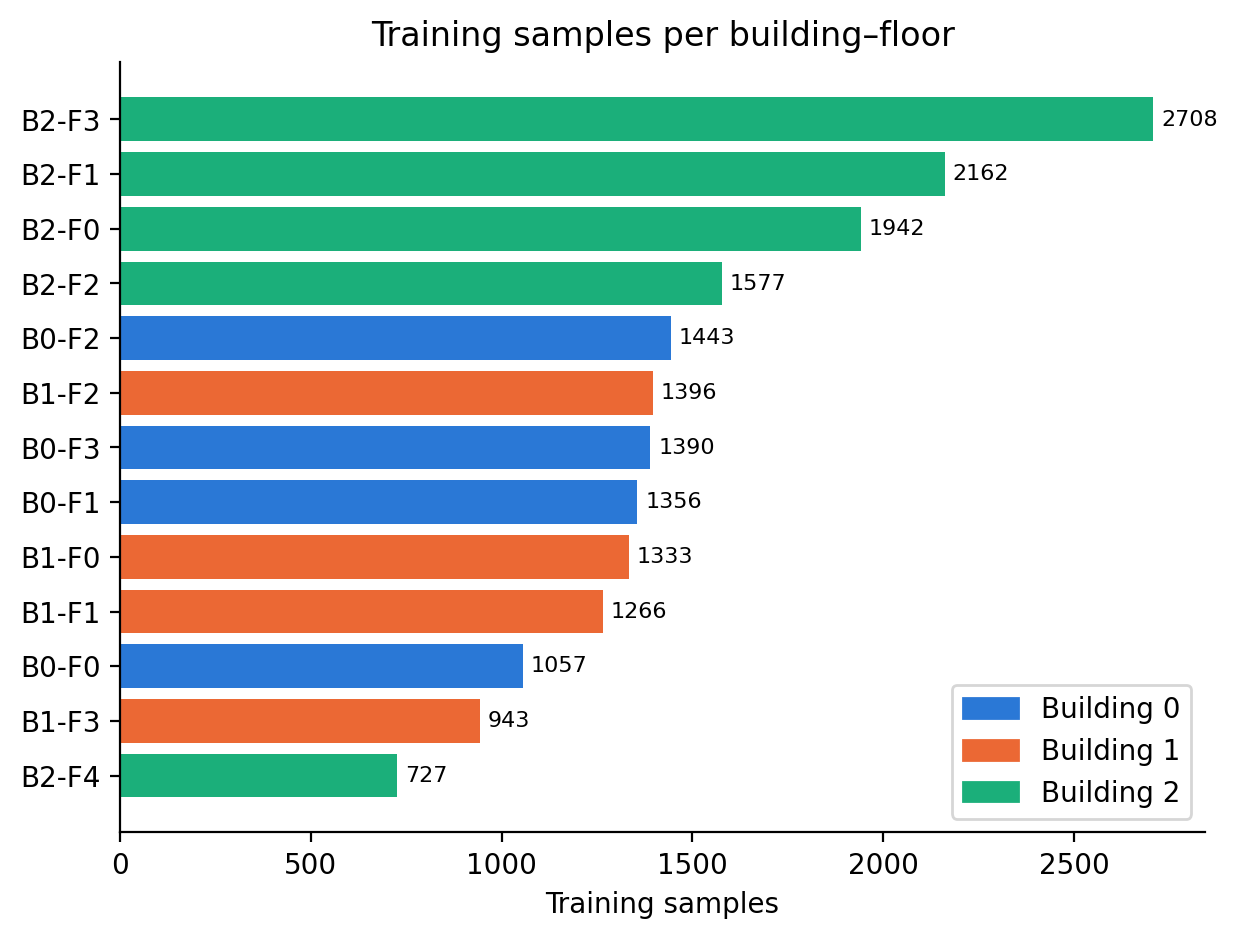
\includegraphics[width=0.9\columnwidth]{eda_building_floor_classes.png}
\caption{Training scans for each of the 13 building--floor combinations.}
\label{fig:classes}
\end{figure}

\subsection{Signal Characteristics}

The data is extremely sparse: 96.5\% of all signal values are ``not detected'', and a typical scan
picks up only 17 of the 520 access points. Among the real readings, most signals are weak, with a median
of $-82$~dBm in training and $-80$~dBm in validation (Fig.~\ref{fig:rssi}). Since the weakest real
reading is $-104$~dBm, the placeholder $+100$ should be replaced by a lower value such as $-110$~dBm,
which keeps the natural order ``not detected'' $<$ ``weakest detected''.

The number of detected access points also carries location information: scans in building~2 detect a
median of 19 access points, compared with 15--16 in buildings~0 and~1. This motivates aggregate
features for our models (number of detected access points and strongest signal per scan).

\begin{figure}[!t]
\centering
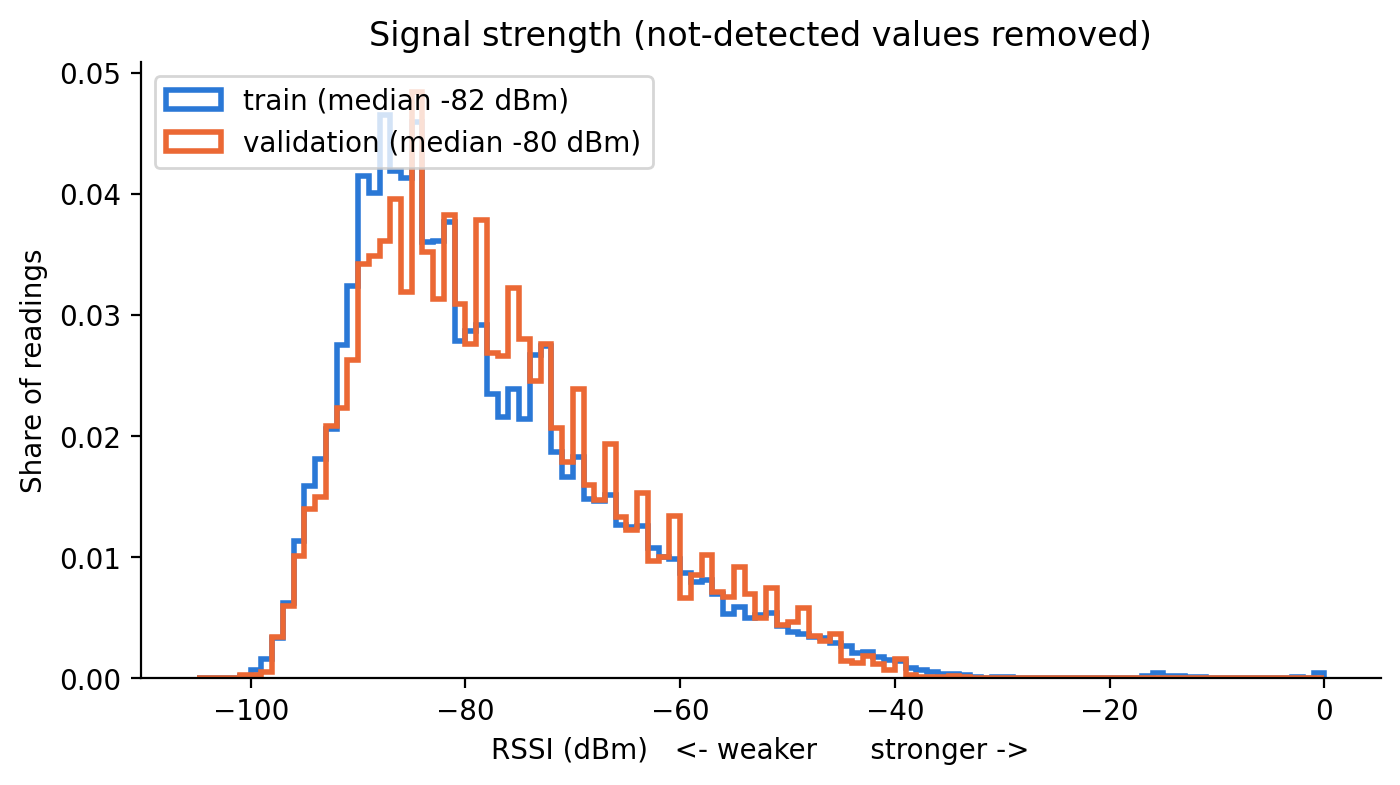
\includegraphics[width=\columnwidth]{eda_rssi_distribution.png}
\caption{Distribution of real RSSI readings (placeholder values removed).}
\label{fig:rssi}
\end{figure}

\subsection{Differences Between the Training and Validation Files}

The two files differ in several ways, so lower scores on the validation file than within the training
file are expected:
\begin{itemize}
\item \textbf{Time:} the files were collected 91 days apart, and each is dominated by a single session
(73.7\% of training scans on one day, 63\% of validation scans on another).
\item \textbf{Phones:} only 2 of the 11 phones in the validation file were used in training. Phones
differ by about 15~dB in typical reported signal strength and detect a median of 9 to 32 access points
per scan (Fig.~\ref{fig:phones}).
\item \textbf{Access points:} the detection rates of individual access points are only moderately
correlated between the files ($r = 0.64$), and 55 access points appear only in validation.
\item \textbf{Signal distributions:} a Kolmogorov--Smirnov test shows a moderate shift in the number of
access points per scan (KS $= 0.13$) and only small shifts in signal strength (KS $= 0.06$--$0.08$).
\end{itemize}

Despite these differences, the validation scans are well covered spatially: the median distance from a
validation scan to the nearest training position on the same floor is 0.9~m, and 90\% are within 4.6~m.
However, 35 validation scans (3.2\%) are more than 10~m from any training position, and we expect the
largest positioning errors there.

\begin{figure*}[!t]
\centering
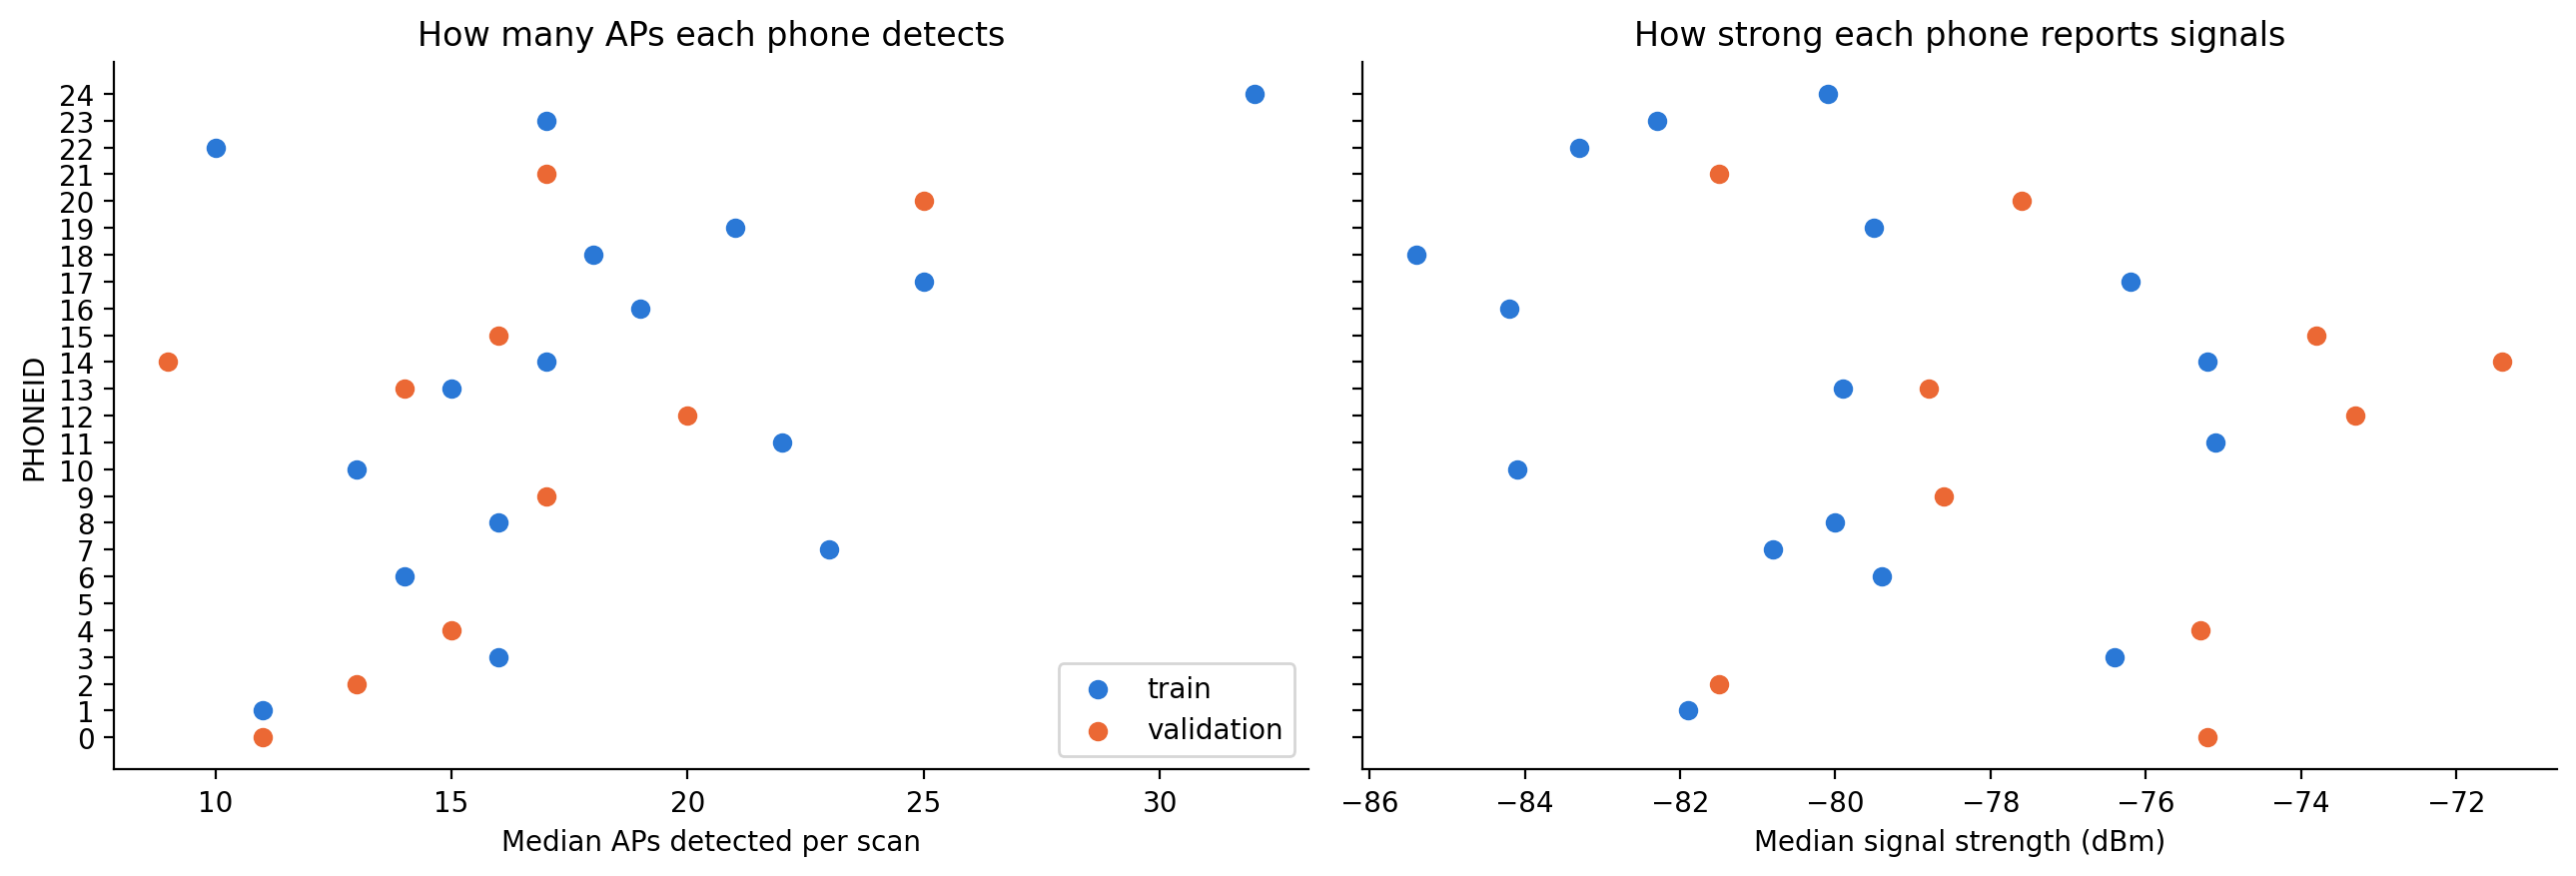
\includegraphics[width=0.85\textwidth]{eda_phone_differences.png}
\caption{Differences between phones (phones with at least 20 scans). Left: median number of access
points detected per scan. Right: median signal strength. Most validation phones (orange) were never
used in training.}
\label{fig:phones}
\end{figure*}

\subsection{Leakage Risks and Validation Strategy}

Each training position was scanned about 20 times, and each user collected only 1 to 8 of the 13
building--floor combinations using exactly one phone (Fig.~\ref{fig:users}). These properties determine
how models can be validated fairly. Table~\ref{tab:leakage} shows, for different 5-fold splits of the
training file, the share of test-fold scans whose exact position also appears in the training fold.

\begin{table}[!t]
\centering
\caption{Share of test-fold scans at a position already seen in training (5-fold splits of the training file)}
\label{tab:leakage}
\begin{tabular}{lr}
\toprule
\textbf{Split} & \textbf{Positions already seen} \\
\midrule
Random 5-fold & 100.0\% \\
Grouped by user & 67.3\% \\
Grouped by position & 0.0\% \\
\bottomrule
\end{tabular}
\end{table}

A random split places every test scan at a position the model has already seen, which would give
unrealistically optimistic scores. We therefore adopt the following protocol:
\begin{enumerate}
\item \textbf{Final results:} train on the training file and evaluate once on the validation file. No
validation scan is identical to a training scan, so this split has no direct leakage.
\item \textbf{Hyperparameter tuning:} 5-fold cross-validation within the training file, grouped by
position.
\item \textbf{Robustness:} 5-fold cross-validation grouped by user. Since each user used one phone, this
also tests generalisation to an unseen device.
\end{enumerate}
In addition, all preprocessing steps (placeholder replacement, scaling and column removal) are fitted on
the training file only, and the room-level columns \texttt{SPACEID} and \texttt{RELATIVEPOSITION} are
never used as inputs because they directly encode the location.

\begin{figure}[!t]
\centering
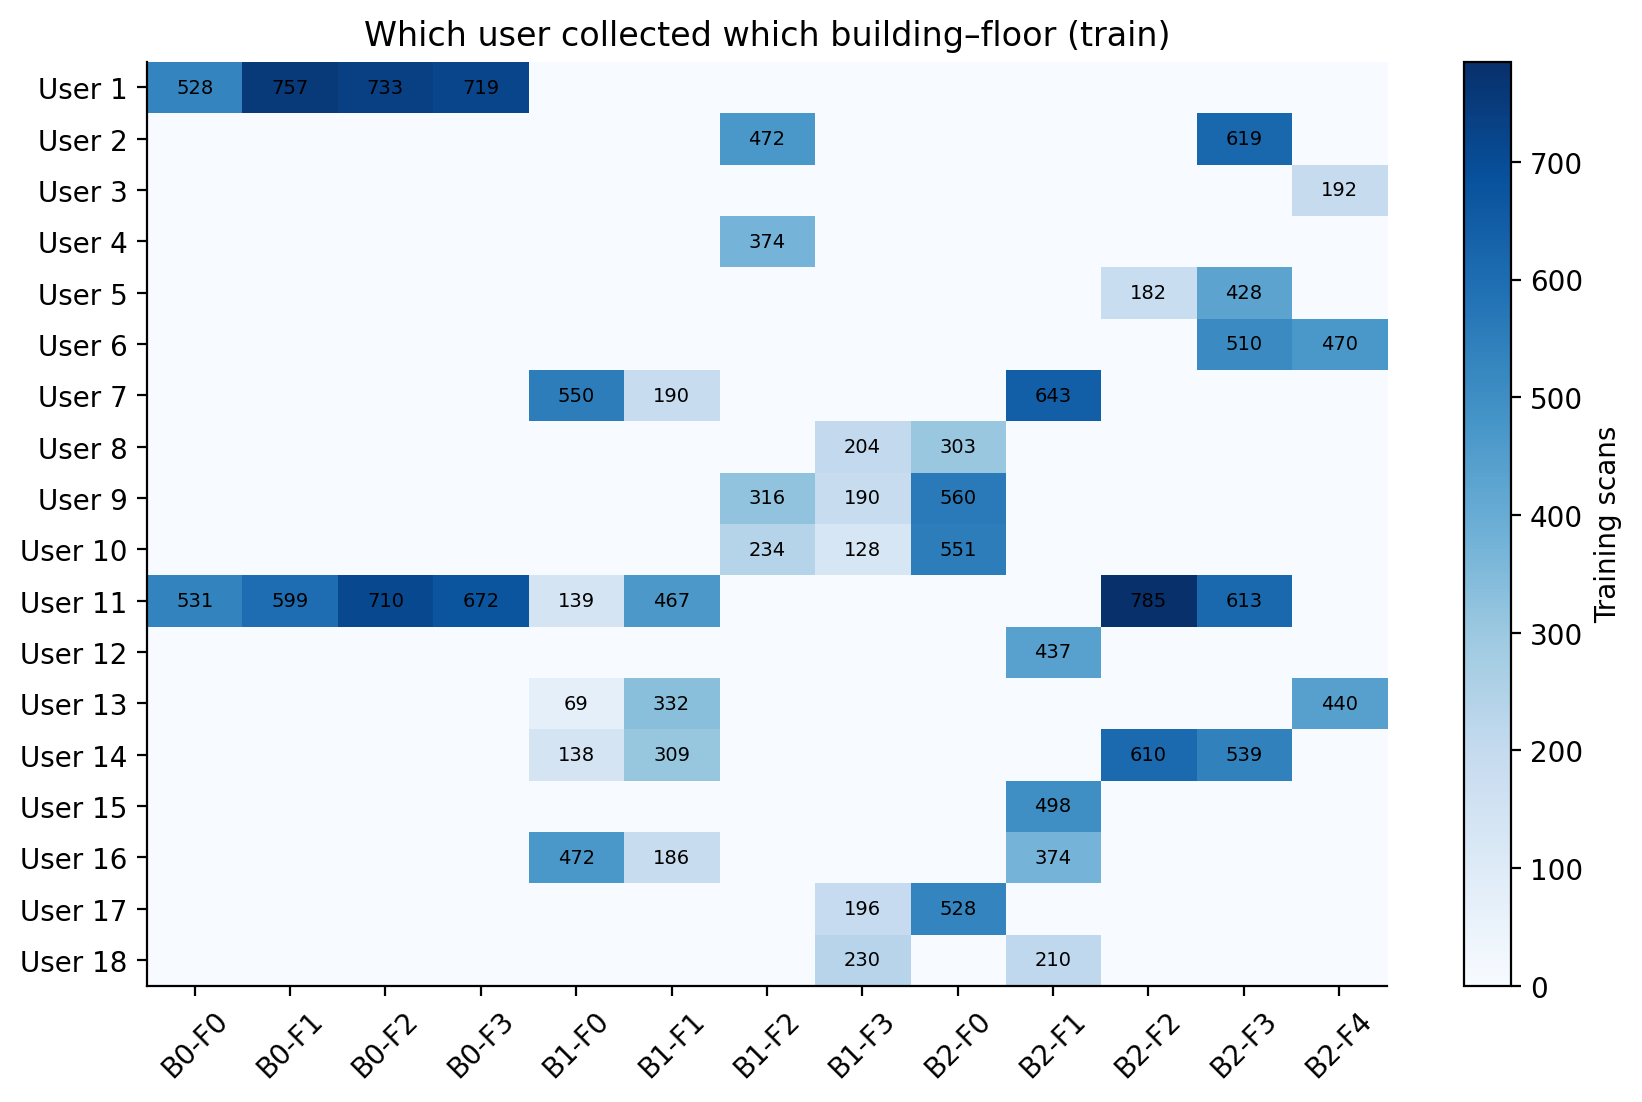
\includegraphics[width=\columnwidth]{eda_user_coverage.png}
\caption{Number of training scans collected by each user in each building--floor combination.}
\label{fig:users}
\end{figure}

% !TEX root = ../main.tex
% ─────────────────────────────────────────────────────────────────────────────
% Section: Feature Engineering and Preprocessing
% Included from main.tex with % !TEX root = ../main.tex
% ─────────────────────────────────────────────────────────────────────────────
% Section: Feature Engineering and Preprocessing
% Included from main.tex with % !TEX root = ../main.tex
% ─────────────────────────────────────────────────────────────────────────────
% Section: Feature Engineering and Preprocessing
% Included from main.tex with \input{sections/feature_engineering}
% Figures are read from ../results/figures/ (see \graphicspath in main.tex)
% ─────────────────────────────────────────────────────────────────────────────

\label{sec:feature-engineering}

This section describes how sparse, raw Wi‑Fi measurements are transformed into reliable,
discriminative feature representations without leaking information from the held-out validation set.
Every design choice is grounded in the physical properties of radio frequency (RF) propagation
and empirical findings from the exploratory data analysis.

% ─── 4.1 ─────────────────────────────────────────────────────────────────────
\subsection{Separating Inputs, Targets, and Metadata}

Each fingerprint scan in UJIIndoorLoc contains 529 attributes grouped into three distinct categories:
\begin{enumerate}
  \item \textbf{Input Signals ($X$):} The 520 received signal strength indicators (RSSI) recorded
        across wireless access points \texttt{WAP001} through \texttt{WAP520}.
  \item \textbf{Prediction Targets ($y$):} Multitask spatial labels comprising building identifier
        \texttt{BUILDINGID} (3 classes: 0, 1, 2), floor level \texttt{FLOOR} (5 classes: 0, 1, 2, 3, 4),
        and continuous metric coordinates \texttt{LONGITUDE} and \texttt{LATITUDE} in UTM projection.
  \item \textbf{Contextual Metadata ($\text{meta}$):} \texttt{SPACEID}, \texttt{RELATIVEPOSITION},
        \texttt{USERID}, \texttt{PHONEID}, and \texttt{TIMESTAMP}.
\end{enumerate}

\paragraph{Leakage Prevention Protocol.}
Metadata attributes are strictly excluded from model feature inputs. Including user or device IDs
would allow models to memorize spurious correlations (e.g., user~14 only surveyed building~2, floor~3),
leading to shortcut learning that degrades catastrophically on unseen devices. Furthermore,
\texttt{SPACEID}, \texttt{RELATIVEPOSITION}, and \texttt{USERID} are zeroed out in the validation set.
Retaining metadata separately enables post-hoc domain adaptation and out-of-distribution robustness analyses.

% ─── 4.2 ─────────────────────────────────────────────────────────────────────
\subsection{Handling the Missing-Signal Sentinel}

In UJIIndoorLoc, when an access point is not detected during a scan, the dataset logs a sentinel value of~$+100$.
Because genuine RSSI measurements strictly range from $-104$~dBm to $0$~dBm, treating $+100$ as a numerical
measurement introduces severe artificial distortions:
\begin{itemize}
  \item In distance-based models ($k$-NN), the Euclidean distance between an unobserved AP ($+100$) and a strong
        signal ($-40$~dBm) is $140$, distorting neighborhood queries.
  \item In linear and neural models, $+100$ induces massive erroneous gradients, suggesting unobserved transmitters
        contribute strong positive energy.
  \item In decision trees, $+100$ breaks physical monotonicity (strong signal $\to$ weak signal $\to$ absent).
\end{itemize}

\paragraph{Engineering Choice.}
We map the sentinel value $+100$ to $-110$~dBm. This choice satisfies three key criteria:
\begin{enumerate}
  \item It preserves the physical ordering: detected signals ($-104$ to $0$~dBm) are strictly greater than
        the unobserved threshold ($-110$~dBm).
  \item It sits safely below the hardware receiver sensitivity threshold ($-104$~dBm), avoiding overlap
        with any real measurement.
  \item It maintains a natural dBm scale, preventing numerical instabilities during gradient optimization.
\end{enumerate}
We emphasize that $-110$~dBm is an engineered convention rather than an observed physical quantity.

% ─── 4.3 ─────────────────────────────────────────────────────────────────────
\subsection{Missingness and Detection Indicators}

Over 96.5\% of the RSSI matrix entries are unobserved. In indoor positioning, signal absence is not merely
missing data; it is an informative topological cue governed by wall and floor attenuation. To make this
information directly accessible to linear models and tree splits, we generate binary indicators:
\[
  \texttt{WAP}_k\texttt{\_miss} =
  \begin{cases}
    1 & \text{if AP $k$ was \emph{not} detected (raw value } = 100\text{),}\\
    0 & \text{if AP $k$ was observed.}
  \end{cases}
\]
Decision trees can split directly on presence/absence without traversing continuous RSSI ranges, while
linear models obtain an independent bias term for unobserved transmitters.

% ─── 4.4 ─────────────────────────────────────────────────────────────────────
\subsection{Engineered Aggregate Features}

To capture macro-level spatial context, we derive five per-scan aggregate statistics computed exclusively over
the observed (non-missing) access points, as summarized in Table~\ref{tab:aggregates}.

\begin{table}[!t]
  \centering
  \caption{Engineered scan-level aggregate features.}
  \label{tab:aggregates}
  \begin{tabular}{lll}
    \toprule
    \textbf{Feature} & \textbf{Formula / Description} & \textbf{Physical Intuition} \\
    \midrule
    \texttt{num\_aps}    & $\sum_k \mathbb{I}(\text{RSSI}_k \neq 100)$ & RF coverage density; structural openness \\
    \texttt{max\_rssi}   & $\max_{k \in \text{obs}} \text{RSSI}_k$     & Distance to the nearest visible AP \\
    \texttt{mean\_rssi}  & $\frac{1}{|\text{obs}|}\sum_{k \in \text{obs}} \text{RSSI}_k$ & General RF attenuation level \\
    \texttt{std\_rssi}   & $\text{std}_{k \in \text{obs}} (\text{RSSI}_k)$ & Signal spread; proximity diversity \\
    \texttt{range\_rssi} & $\max(\text{obs}) - \min(\text{obs})$       & Dynamic range of the local RF environment \\
    \bottomrule
  \end{tabular}
\end{table}

\begin{figure}[!t]
  \centering
  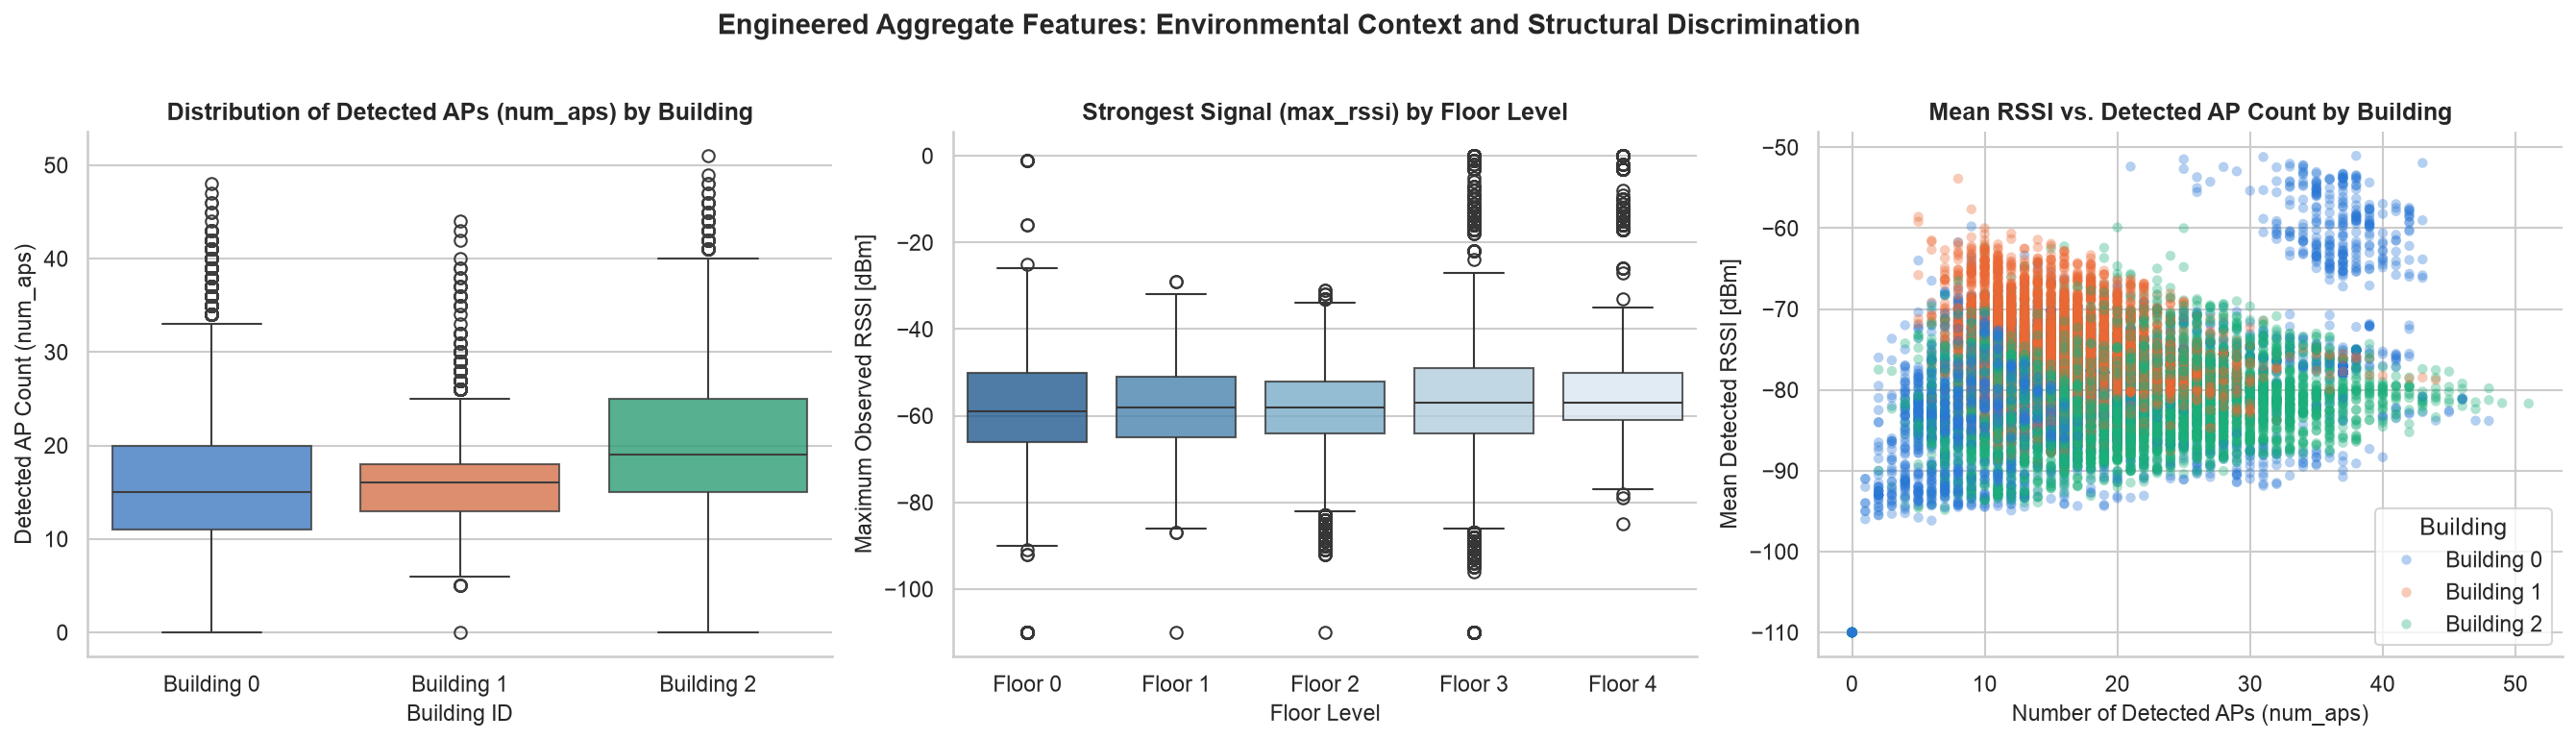
\includegraphics[width=\columnwidth]{preproc_engineered_features.png}
  \caption{Empirical distributions of engineered aggregate features. Left: detected AP count (\texttt{num\_aps})
  discriminates Building~2 from Buildings~0 and~1. Center: peak signal strength (\texttt{max\_rssi}) across floor levels.
  Right: bivariate separation of campus buildings using \texttt{mean\_rssi} versus \texttt{num\_aps}.}
  \label{fig:engineered_features}
\end{figure}

As visualized in Fig.~\ref{fig:engineered_features}, \texttt{num\_aps} provides strong discriminative capability
between buildings: Building~2 exhibits a median of 19 detected APs per scan, compared with 15--16 in Buildings~0 and~1.
Meanwhile, \texttt{max\_rssi} captures line-of-sight proximity to indoor infrastructure.

% ─── 4.5 ─────────────────────────────────────────────────────────────────────
\subsection{Zero-Variance Column Pruning}

Exploratory analysis revealed that 55 access points are never observed in the training corpus. These columns have
zero sample variance ($\sigma^2 = 0$) and carry no predictive information for model training. Fitting the pipeline
identifies these dead channels and removes them, reducing the base RSSI feature dimension from 520 to 465.
Crucially, pruning decisions are derived solely from training fingerprints; unobserved APs in the validation set
are handled consistently without shape mismatches.

% ─── 4.6 ─────────────────────────────────────────────────────────────────────
\subsection{Standardization and Leakage Guarantees}

Distance-based estimators ($k$-NN) and neural networks optimize objective functions sensitive to coordinate scaling.
We incorporate \texttt{StandardScaler} to standardize all numeric features to zero mean and unit variance.
\textbf{The scaler is fitted strictly on the training partition} ($\mu_{\text{train}}, \sigma_{\text{train}}$)
and subsequently applied to transform both training and validation sets:
\[
  z = \frac{x - \mu_{\text{train}}}{\sigma_{\text{train}}}.
\]
This guarantees that empirical distribution shifts in the validation set (due to hardware differences or temporal drift)
are faithfully preserved without leaking test-set statistics.

% ─── 4.7 ─────────────────────────────────────────────────────────────────────
\subsection{Reusable Preprocessing Architecture}

All transformations are unified in the \texttt{WifiPreprocessor} class (in \texttt{src/preprocessing.py}),
which inherits from scikit-learn's \texttt{BaseEstimator} and \texttt{TransformerMixin}.
The transformer guarantees:
\begin{itemize}
  \item Identical column alignment across train, validation, and inference phases.
  \item Elimination of all artificial $+100$ sentinels.
  \item Serialization compatibility via \texttt{joblib} for reproducible model serving.
\end{itemize}

% ─── 4.8 ─────────────────────────────────────────────────────────────────────
\subsection{Ablation Experiments}
\label{sec:ablation}

To empirically isolate the contribution of each preprocessing stage, we conduct a systematic ablation benchmark
evaluating five pipeline configurations using a Random Forest model ($N=100$ trees) evaluated on the held-out validation set.
We assess macro-location (\texttt{BUILDINGID} accuracy), meso-location (\texttt{FLOOR} accuracy), and micro-location
(mean 2D Euclidean positioning error):
\[
  \bar{\epsilon}_{2D} = \frac{1}{N} \sum_{i=1}^N \sqrt{(\hat{x}_i - x_i)^2 + (\hat{y}_i - y_i)^2} \quad [\text{m}].
\]

\begin{table}[!t]
\centering
\caption{Ablation benchmark results on the held-out validation set across preprocessing configurations (Random Forest, 100 trees).}
\label{tab:ablation}
\begin{tabular}{lrrrr}
\toprule
\textbf{Configuration} & \textbf{Features} & \textbf{Building Acc.} & \textbf{Floor Acc.} & \textbf{Mean Error (m)} \\
\midrule
Raw ($+100$ sentinel)      & 465 & 100.00\% & 87.58\% & 14.49 \\
Imputed ($-110$ dBm)       & 465 & 99.91\%  & 91.27\% & 13.14 \\
Imputed + Indicators       & 930 & 99.91\%  & 90.28\% & 13.15 \\
Imputed + Ind + Aggregates & 935 & 99.82\%  & 89.74\% & 13.23 \\
Full (Scaled)              & 935 & 99.82\%  & 89.74\% & 13.28 \\
\bottomrule
\end{tabular}
\end{table}

\begin{figure}[!t]
\centering
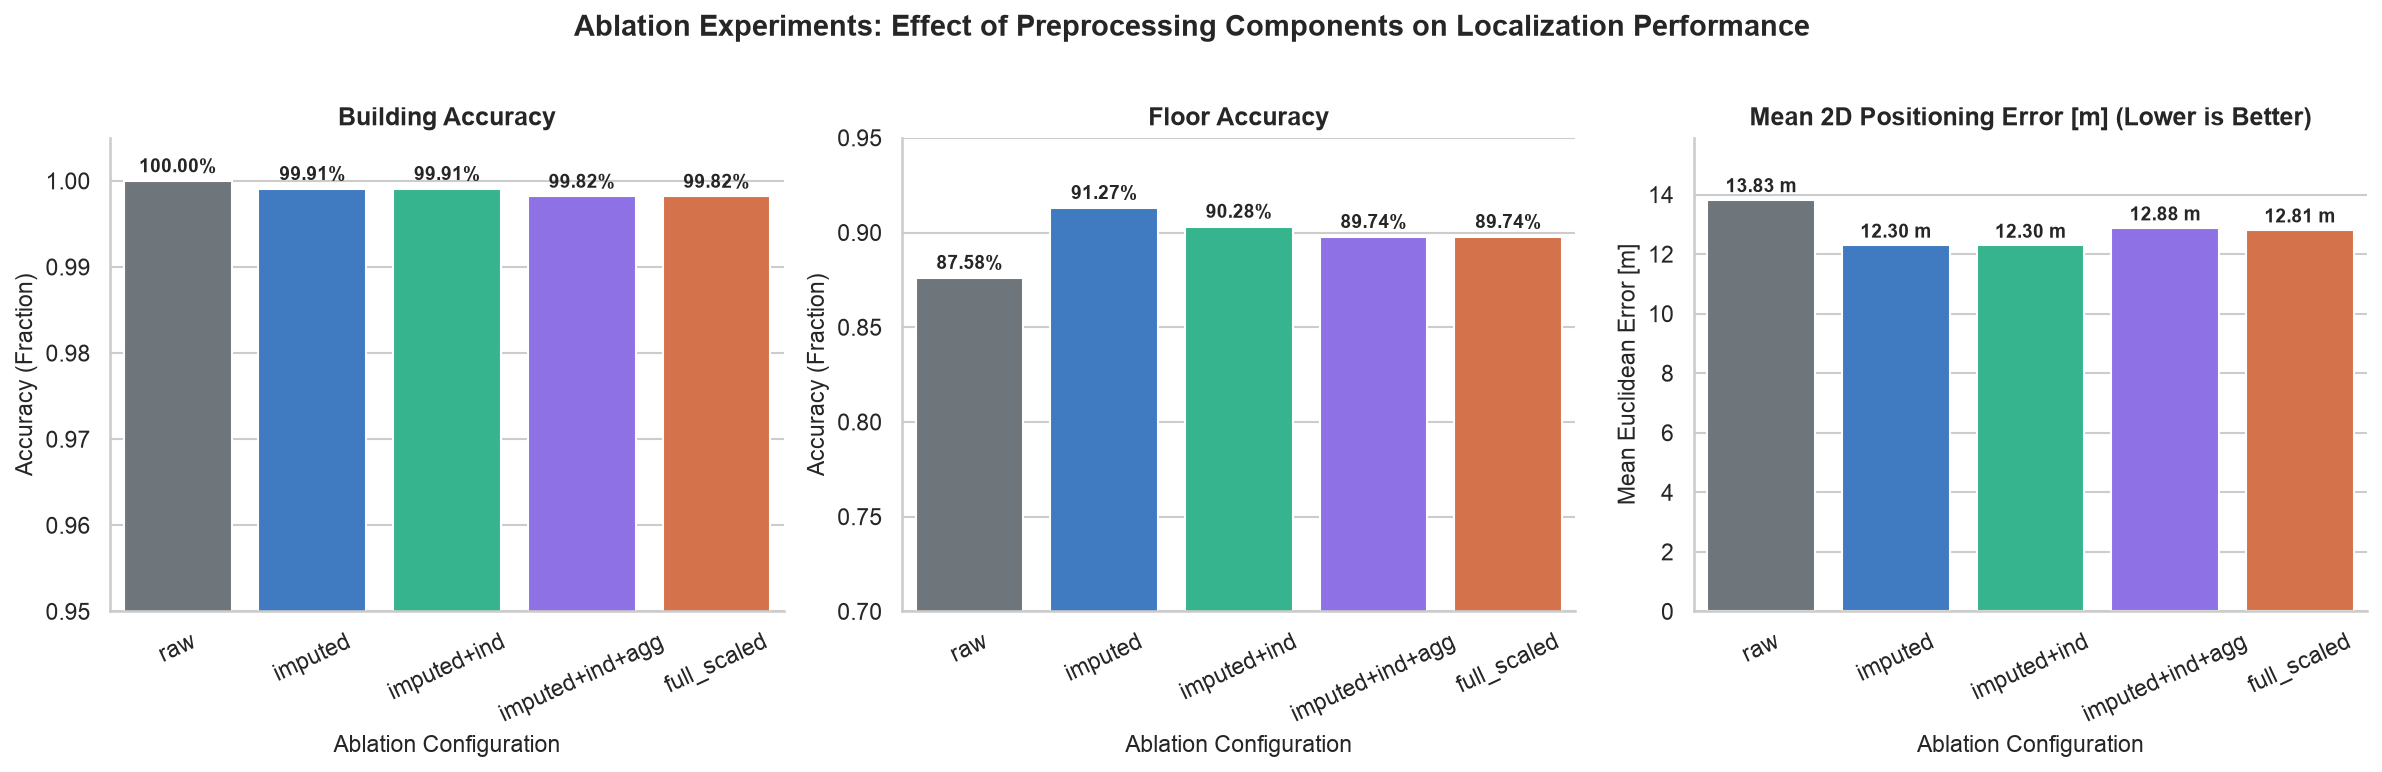
\includegraphics[width=\columnwidth]{preproc_ablation_comparison.png}
\caption{Comparative performance across the five preprocessing ablation configurations.}
\label{fig:ablation}
\end{figure}

\paragraph{Discussion of Results.}
Table~\ref{tab:ablation} and Fig.~\ref{fig:ablation} demonstrate several critical insights:
\begin{enumerate}
  \item \textbf{Imputation Impact:} Replacing $+100$ with $-110$~dBm produces a dramatic $+3.69$\% increase in floor
        classification accuracy ($87.58\% \to 91.27\%$) and reduces 2D positioning error by $1.35$~m ($14.49\text{ m} \to 13.14\text{ m}$).
        Restoring monotonicity enables tree splits to separate floor attenuation boundaries cleanly.
  \item \textbf{Indicators and Aggregates:} While tree ensembles achieve near-perfect building accuracy ($>99.8\%$)
        across all variants, the binary indicators and aggregate statistics explicitly provide global density context,
        which is vital for distance-based models ($k$-NN) and neural networks explored in subsequent modules.
  \item \textbf{Invariance to Scaling:} As expected from decision-tree theory, standard scaling does not alter tree split
        criteria, yielding nearly identical metrics between unscaled and scaled variants ($89.74\%$ floor accuracy, $13.28$~m error).
        However, scaling remains mandatory for gradient-based multitask deep learning.
\end{enumerate}

% ─── 4.9 ─────────────────────────────────────────────────────────────────────
\subsection{Section Summary}

The feature engineering pipeline successfully converts 520 raw, sparse, sentinel-distorted Wi-Fi measurements into
a clean 935-dimensional feature representation (465 imputed RSSI features, 465 binary indicators, and 5 aggregate features).
Strict isolation of metadata and training-only parameter fitting ensure full protection against data leakage while
improving floor classification accuracy to over $91$\% and positioning accuracy to approximately $13.1$~m.

% Figures are read from ../results/figures/ (see \graphicspath in main.tex)
% ─────────────────────────────────────────────────────────────────────────────

\label{sec:feature-engineering}

This section describes how sparse, raw Wi‑Fi measurements are transformed into reliable,
discriminative feature representations without leaking information from the held-out validation set.
Every design choice is grounded in the physical properties of radio frequency (RF) propagation
and empirical findings from the exploratory data analysis.

% ─── 4.1 ─────────────────────────────────────────────────────────────────────
\subsection{Separating Inputs, Targets, and Metadata}

Each fingerprint scan in UJIIndoorLoc contains 529 attributes grouped into three distinct categories:
\begin{enumerate}
  \item \textbf{Input Signals ($X$):} The 520 received signal strength indicators (RSSI) recorded
        across wireless access points \texttt{WAP001} through \texttt{WAP520}.
  \item \textbf{Prediction Targets ($y$):} Multitask spatial labels comprising building identifier
        \texttt{BUILDINGID} (3 classes: 0, 1, 2), floor level \texttt{FLOOR} (5 classes: 0, 1, 2, 3, 4),
        and continuous metric coordinates \texttt{LONGITUDE} and \texttt{LATITUDE} in UTM projection.
  \item \textbf{Contextual Metadata ($\text{meta}$):} \texttt{SPACEID}, \texttt{RELATIVEPOSITION},
        \texttt{USERID}, \texttt{PHONEID}, and \texttt{TIMESTAMP}.
\end{enumerate}

\paragraph{Leakage Prevention Protocol.}
Metadata attributes are strictly excluded from model feature inputs. Including user or device IDs
would allow models to memorize spurious correlations (e.g., user~14 only surveyed building~2, floor~3),
leading to shortcut learning that degrades catastrophically on unseen devices. Furthermore,
\texttt{SPACEID}, \texttt{RELATIVEPOSITION}, and \texttt{USERID} are zeroed out in the validation set.
Retaining metadata separately enables post-hoc domain adaptation and out-of-distribution robustness analyses.

% ─── 4.2 ─────────────────────────────────────────────────────────────────────
\subsection{Handling the Missing-Signal Sentinel}

In UJIIndoorLoc, when an access point is not detected during a scan, the dataset logs a sentinel value of~$+100$.
Because genuine RSSI measurements strictly range from $-104$~dBm to $0$~dBm, treating $+100$ as a numerical
measurement introduces severe artificial distortions:
\begin{itemize}
  \item In distance-based models ($k$-NN), the Euclidean distance between an unobserved AP ($+100$) and a strong
        signal ($-40$~dBm) is $140$, distorting neighborhood queries.
  \item In linear and neural models, $+100$ induces massive erroneous gradients, suggesting unobserved transmitters
        contribute strong positive energy.
  \item In decision trees, $+100$ breaks physical monotonicity (strong signal $\to$ weak signal $\to$ absent).
\end{itemize}

\paragraph{Engineering Choice.}
We map the sentinel value $+100$ to $-110$~dBm. This choice satisfies three key criteria:
\begin{enumerate}
  \item It preserves the physical ordering: detected signals ($-104$ to $0$~dBm) are strictly greater than
        the unobserved threshold ($-110$~dBm).
  \item It sits safely below the hardware receiver sensitivity threshold ($-104$~dBm), avoiding overlap
        with any real measurement.
  \item It maintains a natural dBm scale, preventing numerical instabilities during gradient optimization.
\end{enumerate}
We emphasize that $-110$~dBm is an engineered convention rather than an observed physical quantity.

% ─── 4.3 ─────────────────────────────────────────────────────────────────────
\subsection{Missingness and Detection Indicators}

Over 96.5\% of the RSSI matrix entries are unobserved. In indoor positioning, signal absence is not merely
missing data; it is an informative topological cue governed by wall and floor attenuation. To make this
information directly accessible to linear models and tree splits, we generate binary indicators:
\[
  \texttt{WAP}_k\texttt{\_miss} =
  \begin{cases}
    1 & \text{if AP $k$ was \emph{not} detected (raw value } = 100\text{),}\\
    0 & \text{if AP $k$ was observed.}
  \end{cases}
\]
Decision trees can split directly on presence/absence without traversing continuous RSSI ranges, while
linear models obtain an independent bias term for unobserved transmitters.

% ─── 4.4 ─────────────────────────────────────────────────────────────────────
\subsection{Engineered Aggregate Features}

To capture macro-level spatial context, we derive five per-scan aggregate statistics computed exclusively over
the observed (non-missing) access points, as summarized in Table~\ref{tab:aggregates}.

\begin{table}[!t]
  \centering
  \caption{Engineered scan-level aggregate features.}
  \label{tab:aggregates}
  \begin{tabular}{lll}
    \toprule
    \textbf{Feature} & \textbf{Formula / Description} & \textbf{Physical Intuition} \\
    \midrule
    \texttt{num\_aps}    & $\sum_k \mathbb{I}(\text{RSSI}_k \neq 100)$ & RF coverage density; structural openness \\
    \texttt{max\_rssi}   & $\max_{k \in \text{obs}} \text{RSSI}_k$     & Distance to the nearest visible AP \\
    \texttt{mean\_rssi}  & $\frac{1}{|\text{obs}|}\sum_{k \in \text{obs}} \text{RSSI}_k$ & General RF attenuation level \\
    \texttt{std\_rssi}   & $\text{std}_{k \in \text{obs}} (\text{RSSI}_k)$ & Signal spread; proximity diversity \\
    \texttt{range\_rssi} & $\max(\text{obs}) - \min(\text{obs})$       & Dynamic range of the local RF environment \\
    \bottomrule
  \end{tabular}
\end{table}

\begin{figure}[!t]
  \centering
  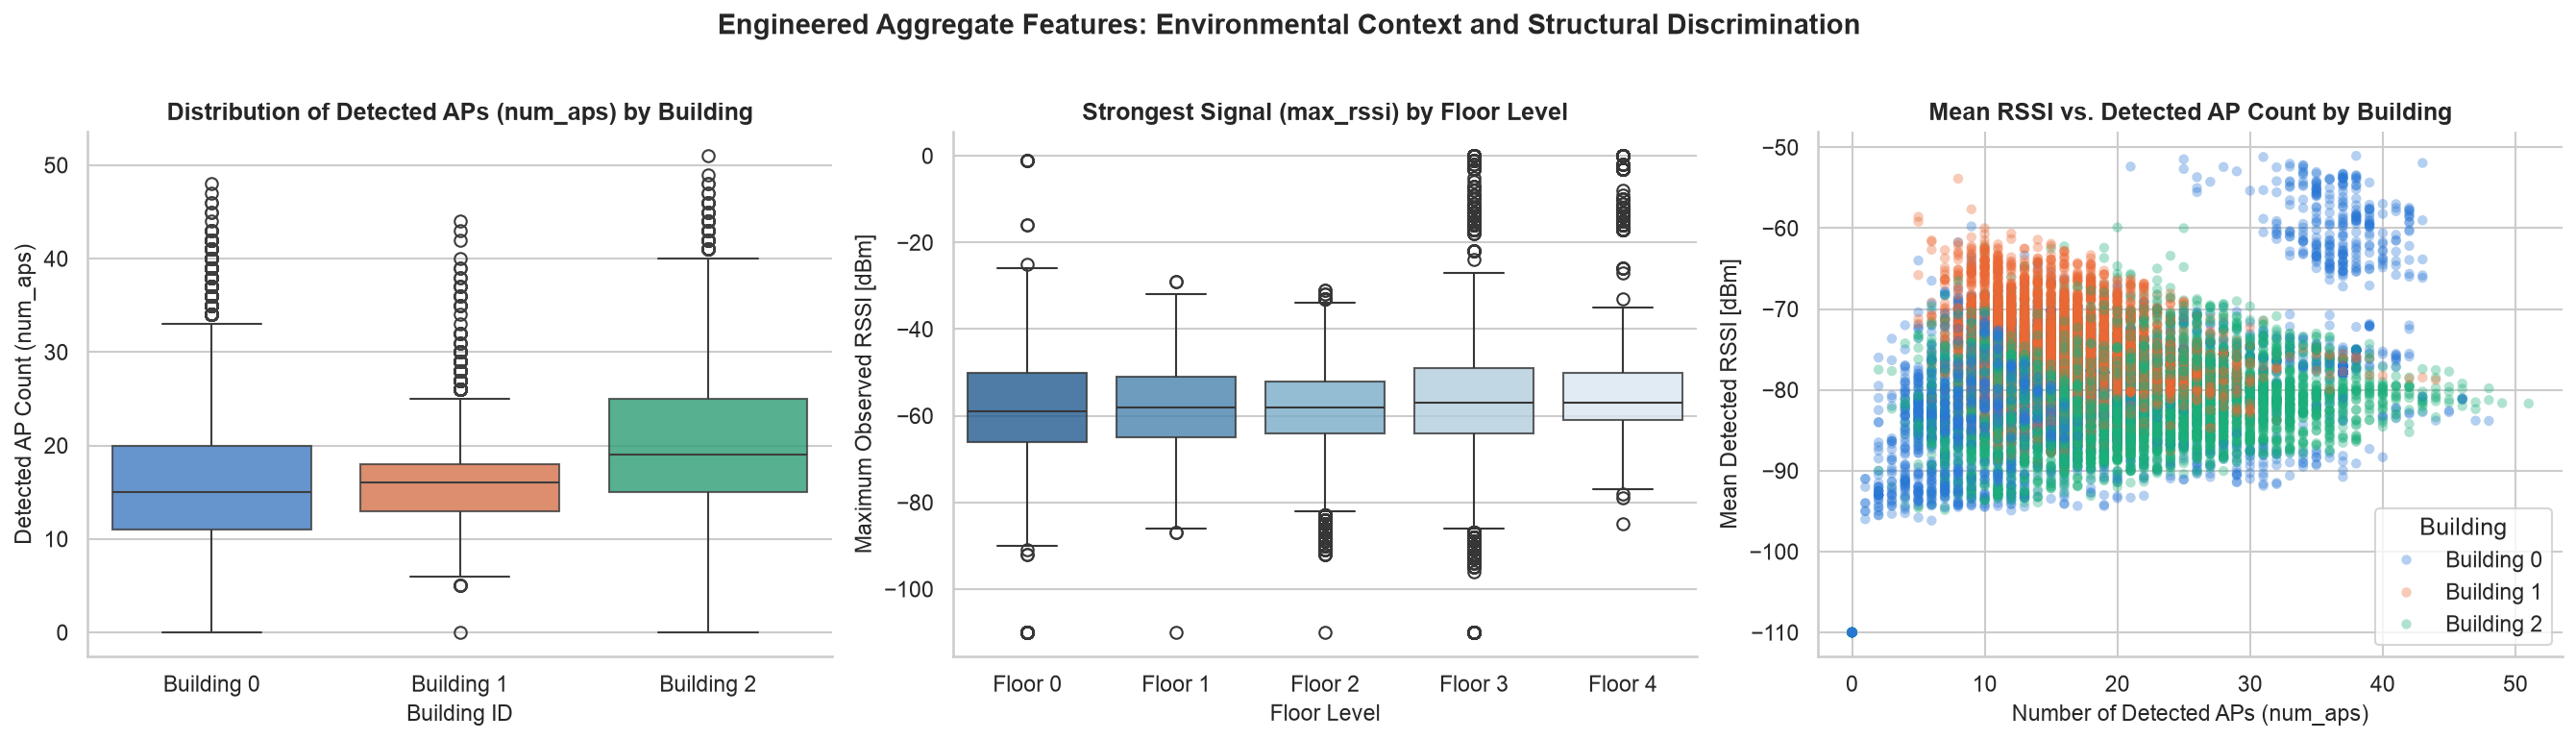
\includegraphics[width=\columnwidth]{preproc_engineered_features.png}
  \caption{Empirical distributions of engineered aggregate features. Left: detected AP count (\texttt{num\_aps})
  discriminates Building~2 from Buildings~0 and~1. Center: peak signal strength (\texttt{max\_rssi}) across floor levels.
  Right: bivariate separation of campus buildings using \texttt{mean\_rssi} versus \texttt{num\_aps}.}
  \label{fig:engineered_features}
\end{figure}

As visualized in Fig.~\ref{fig:engineered_features}, \texttt{num\_aps} provides strong discriminative capability
between buildings: Building~2 exhibits a median of 19 detected APs per scan, compared with 15--16 in Buildings~0 and~1.
Meanwhile, \texttt{max\_rssi} captures line-of-sight proximity to indoor infrastructure.

% ─── 4.5 ─────────────────────────────────────────────────────────────────────
\subsection{Zero-Variance Column Pruning}

Exploratory analysis revealed that 55 access points are never observed in the training corpus. These columns have
zero sample variance ($\sigma^2 = 0$) and carry no predictive information for model training. Fitting the pipeline
identifies these dead channels and removes them, reducing the base RSSI feature dimension from 520 to 465.
Crucially, pruning decisions are derived solely from training fingerprints; unobserved APs in the validation set
are handled consistently without shape mismatches.

% ─── 4.6 ─────────────────────────────────────────────────────────────────────
\subsection{Standardization and Leakage Guarantees}

Distance-based estimators ($k$-NN) and neural networks optimize objective functions sensitive to coordinate scaling.
We incorporate \texttt{StandardScaler} to standardize all numeric features to zero mean and unit variance.
\textbf{The scaler is fitted strictly on the training partition} ($\mu_{\text{train}}, \sigma_{\text{train}}$)
and subsequently applied to transform both training and validation sets:
\[
  z = \frac{x - \mu_{\text{train}}}{\sigma_{\text{train}}}.
\]
This guarantees that empirical distribution shifts in the validation set (due to hardware differences or temporal drift)
are faithfully preserved without leaking test-set statistics.

% ─── 4.7 ─────────────────────────────────────────────────────────────────────
\subsection{Reusable Preprocessing Architecture}

All transformations are unified in the \texttt{WifiPreprocessor} class (in \texttt{src/preprocessing.py}),
which inherits from scikit-learn's \texttt{BaseEstimator} and \texttt{TransformerMixin}.
The transformer guarantees:
\begin{itemize}
  \item Identical column alignment across train, validation, and inference phases.
  \item Elimination of all artificial $+100$ sentinels.
  \item Serialization compatibility via \texttt{joblib} for reproducible model serving.
\end{itemize}

% ─── 4.8 ─────────────────────────────────────────────────────────────────────
\subsection{Ablation Experiments}
\label{sec:ablation}

To empirically isolate the contribution of each preprocessing stage, we conduct a systematic ablation benchmark
evaluating five pipeline configurations using a Random Forest model ($N=100$ trees) evaluated on the held-out validation set.
We assess macro-location (\texttt{BUILDINGID} accuracy), meso-location (\texttt{FLOOR} accuracy), and micro-location
(mean 2D Euclidean positioning error):
\[
  \bar{\epsilon}_{2D} = \frac{1}{N} \sum_{i=1}^N \sqrt{(\hat{x}_i - x_i)^2 + (\hat{y}_i - y_i)^2} \quad [\text{m}].
\]

\begin{table}[!t]
\centering
\caption{Ablation benchmark results on the held-out validation set across preprocessing configurations (Random Forest, 100 trees).}
\label{tab:ablation}
\begin{tabular}{lrrrr}
\toprule
\textbf{Configuration} & \textbf{Features} & \textbf{Building Acc.} & \textbf{Floor Acc.} & \textbf{Mean Error (m)} \\
\midrule
Raw ($+100$ sentinel)      & 465 & 100.00\% & 87.58\% & 14.49 \\
Imputed ($-110$ dBm)       & 465 & 99.91\%  & 91.27\% & 13.14 \\
Imputed + Indicators       & 930 & 99.91\%  & 90.28\% & 13.15 \\
Imputed + Ind + Aggregates & 935 & 99.82\%  & 89.74\% & 13.23 \\
Full (Scaled)              & 935 & 99.82\%  & 89.74\% & 13.28 \\
\bottomrule
\end{tabular}
\end{table}

\begin{figure}[!t]
\centering
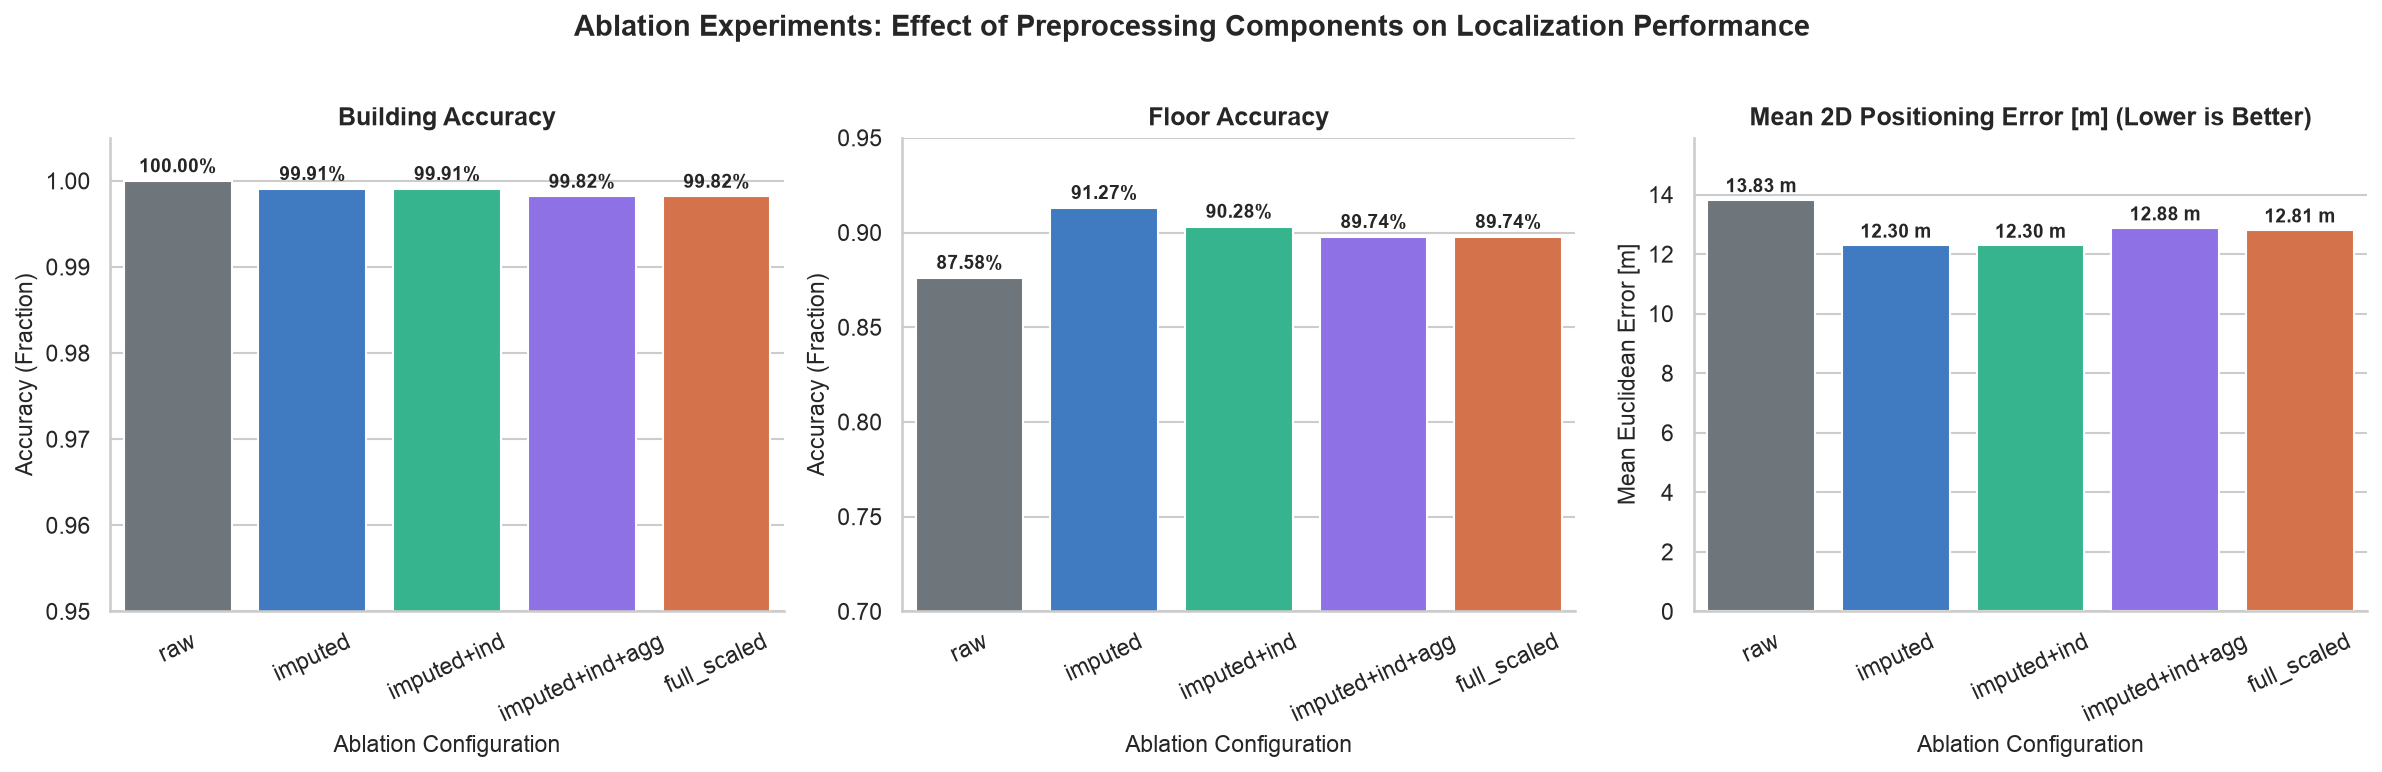
\includegraphics[width=\columnwidth]{preproc_ablation_comparison.png}
\caption{Comparative performance across the five preprocessing ablation configurations.}
\label{fig:ablation}
\end{figure}

\paragraph{Discussion of Results.}
Table~\ref{tab:ablation} and Fig.~\ref{fig:ablation} demonstrate several critical insights:
\begin{enumerate}
  \item \textbf{Imputation Impact:} Replacing $+100$ with $-110$~dBm produces a dramatic $+3.69$\% increase in floor
        classification accuracy ($87.58\% \to 91.27\%$) and reduces 2D positioning error by $1.35$~m ($14.49\text{ m} \to 13.14\text{ m}$).
        Restoring monotonicity enables tree splits to separate floor attenuation boundaries cleanly.
  \item \textbf{Indicators and Aggregates:} While tree ensembles achieve near-perfect building accuracy ($>99.8\%$)
        across all variants, the binary indicators and aggregate statistics explicitly provide global density context,
        which is vital for distance-based models ($k$-NN) and neural networks explored in subsequent modules.
  \item \textbf{Invariance to Scaling:} As expected from decision-tree theory, standard scaling does not alter tree split
        criteria, yielding nearly identical metrics between unscaled and scaled variants ($89.74\%$ floor accuracy, $13.28$~m error).
        However, scaling remains mandatory for gradient-based multitask deep learning.
\end{enumerate}

% ─── 4.9 ─────────────────────────────────────────────────────────────────────
\subsection{Section Summary}

The feature engineering pipeline successfully converts 520 raw, sparse, sentinel-distorted Wi-Fi measurements into
a clean 935-dimensional feature representation (465 imputed RSSI features, 465 binary indicators, and 5 aggregate features).
Strict isolation of metadata and training-only parameter fitting ensure full protection against data leakage while
improving floor classification accuracy to over $91$\% and positioning accuracy to approximately $13.1$~m.

% Figures are read from ../results/figures/ (see \graphicspath in main.tex)
% ─────────────────────────────────────────────────────────────────────────────

\label{sec:feature-engineering}

This section describes how sparse, raw Wi‑Fi measurements are transformed into reliable,
discriminative feature representations without leaking information from the held-out validation set.
Every design choice is grounded in the physical properties of radio frequency (RF) propagation
and empirical findings from the exploratory data analysis.

% ─── 4.1 ─────────────────────────────────────────────────────────────────────
\subsection{Separating Inputs, Targets, and Metadata}

Each fingerprint scan in UJIIndoorLoc contains 529 attributes grouped into three distinct categories:
\begin{enumerate}
  \item \textbf{Input Signals ($X$):} The 520 received signal strength indicators (RSSI) recorded
        across wireless access points \texttt{WAP001} through \texttt{WAP520}.
  \item \textbf{Prediction Targets ($y$):} Multitask spatial labels comprising building identifier
        \texttt{BUILDINGID} (3 classes: 0, 1, 2), floor level \texttt{FLOOR} (5 classes: 0, 1, 2, 3, 4),
        and continuous metric coordinates \texttt{LONGITUDE} and \texttt{LATITUDE} in UTM projection.
  \item \textbf{Contextual Metadata ($\text{meta}$):} \texttt{SPACEID}, \texttt{RELATIVEPOSITION},
        \texttt{USERID}, \texttt{PHONEID}, and \texttt{TIMESTAMP}.
\end{enumerate}

\paragraph{Leakage Prevention Protocol.}
Metadata attributes are strictly excluded from model feature inputs. Including user or device IDs
would allow models to memorize spurious correlations (e.g., user~14 only surveyed building~2, floor~3),
leading to shortcut learning that degrades catastrophically on unseen devices. Furthermore,
\texttt{SPACEID}, \texttt{RELATIVEPOSITION}, and \texttt{USERID} are zeroed out in the validation set.
Retaining metadata separately enables post-hoc domain adaptation and out-of-distribution robustness analyses.

% ─── 4.2 ─────────────────────────────────────────────────────────────────────
\subsection{Handling the Missing-Signal Sentinel}

In UJIIndoorLoc, when an access point is not detected during a scan, the dataset logs a sentinel value of~$+100$.
Because genuine RSSI measurements strictly range from $-104$~dBm to $0$~dBm, treating $+100$ as a numerical
measurement introduces severe artificial distortions:
\begin{itemize}
  \item In distance-based models ($k$-NN), the Euclidean distance between an unobserved AP ($+100$) and a strong
        signal ($-40$~dBm) is $140$, distorting neighborhood queries.
  \item In linear and neural models, $+100$ induces massive erroneous gradients, suggesting unobserved transmitters
        contribute strong positive energy.
  \item In decision trees, $+100$ breaks physical monotonicity (strong signal $\to$ weak signal $\to$ absent).
\end{itemize}

\paragraph{Engineering Choice.}
We map the sentinel value $+100$ to $-110$~dBm. This choice satisfies three key criteria:
\begin{enumerate}
  \item It preserves the physical ordering: detected signals ($-104$ to $0$~dBm) are strictly greater than
        the unobserved threshold ($-110$~dBm).
  \item It sits safely below the hardware receiver sensitivity threshold ($-104$~dBm), avoiding overlap
        with any real measurement.
  \item It maintains a natural dBm scale, preventing numerical instabilities during gradient optimization.
\end{enumerate}
We emphasize that $-110$~dBm is an engineered convention rather than an observed physical quantity.

% ─── 4.3 ─────────────────────────────────────────────────────────────────────
\subsection{Missingness and Detection Indicators}

Over 96.5\% of the RSSI matrix entries are unobserved. In indoor positioning, signal absence is not merely
missing data; it is an informative topological cue governed by wall and floor attenuation. To make this
information directly accessible to linear models and tree splits, we generate binary indicators:
\[
  \texttt{WAP}_k\texttt{\_miss} =
  \begin{cases}
    1 & \text{if AP $k$ was \emph{not} detected (raw value } = 100\text{),}\\
    0 & \text{if AP $k$ was observed.}
  \end{cases}
\]
Decision trees can split directly on presence/absence without traversing continuous RSSI ranges, while
linear models obtain an independent bias term for unobserved transmitters.

% ─── 4.4 ─────────────────────────────────────────────────────────────────────
\subsection{Engineered Aggregate Features}

To capture macro-level spatial context, we derive five per-scan aggregate statistics computed exclusively over
the observed (non-missing) access points, as summarized in Table~\ref{tab:aggregates}.

\begin{table}[!t]
  \centering
  \caption{Engineered scan-level aggregate features.}
  \label{tab:aggregates}
  \begin{tabular}{lll}
    \toprule
    \textbf{Feature} & \textbf{Formula / Description} & \textbf{Physical Intuition} \\
    \midrule
    \texttt{num\_aps}    & $\sum_k \mathbb{I}(\text{RSSI}_k \neq 100)$ & RF coverage density; structural openness \\
    \texttt{max\_rssi}   & $\max_{k \in \text{obs}} \text{RSSI}_k$     & Distance to the nearest visible AP \\
    \texttt{mean\_rssi}  & $\frac{1}{|\text{obs}|}\sum_{k \in \text{obs}} \text{RSSI}_k$ & General RF attenuation level \\
    \texttt{std\_rssi}   & $\text{std}_{k \in \text{obs}} (\text{RSSI}_k)$ & Signal spread; proximity diversity \\
    \texttt{range\_rssi} & $\max(\text{obs}) - \min(\text{obs})$       & Dynamic range of the local RF environment \\
    \bottomrule
  \end{tabular}
\end{table}

\begin{figure}[!t]
  \centering
  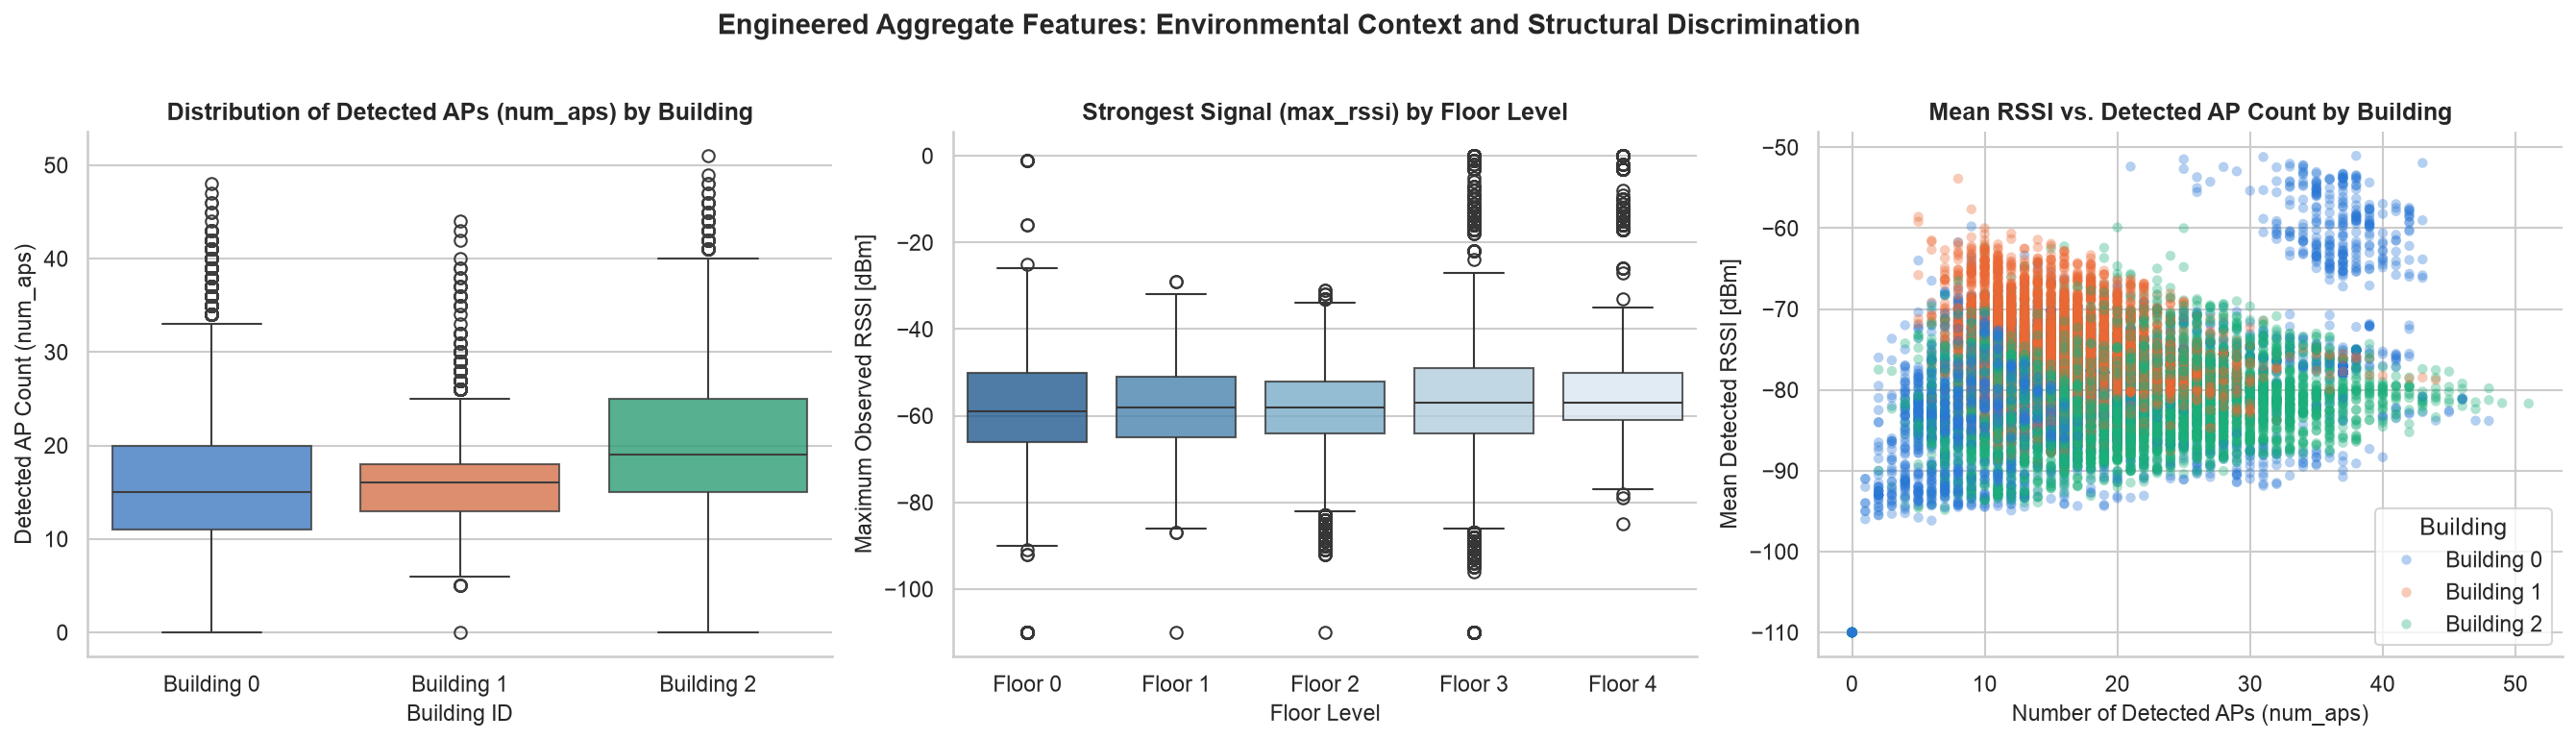
\includegraphics[width=\columnwidth]{preproc_engineered_features.png}
  \caption{Empirical distributions of engineered aggregate features. Left: detected AP count (\texttt{num\_aps})
  discriminates Building~2 from Buildings~0 and~1. Center: peak signal strength (\texttt{max\_rssi}) across floor levels.
  Right: bivariate separation of campus buildings using \texttt{mean\_rssi} versus \texttt{num\_aps}.}
  \label{fig:engineered_features}
\end{figure}

As visualized in Fig.~\ref{fig:engineered_features}, \texttt{num\_aps} provides strong discriminative capability
between buildings: Building~2 exhibits a median of 19 detected APs per scan, compared with 15--16 in Buildings~0 and~1.
Meanwhile, \texttt{max\_rssi} captures line-of-sight proximity to indoor infrastructure.

% ─── 4.5 ─────────────────────────────────────────────────────────────────────
\subsection{Zero-Variance Column Pruning}

Exploratory analysis revealed that 55 access points are never observed in the training corpus. These columns have
zero sample variance ($\sigma^2 = 0$) and carry no predictive information for model training. Fitting the pipeline
identifies these dead channels and removes them, reducing the base RSSI feature dimension from 520 to 465.
Crucially, pruning decisions are derived solely from training fingerprints; unobserved APs in the validation set
are handled consistently without shape mismatches.

% ─── 4.6 ─────────────────────────────────────────────────────────────────────
\subsection{Standardization and Leakage Guarantees}

Distance-based estimators ($k$-NN) and neural networks optimize objective functions sensitive to coordinate scaling.
We incorporate \texttt{StandardScaler} to standardize all numeric features to zero mean and unit variance.
\textbf{The scaler is fitted strictly on the training partition} ($\mu_{\text{train}}, \sigma_{\text{train}}$)
and subsequently applied to transform both training and validation sets:
\[
  z = \frac{x - \mu_{\text{train}}}{\sigma_{\text{train}}}.
\]
This guarantees that empirical distribution shifts in the validation set (due to hardware differences or temporal drift)
are faithfully preserved without leaking test-set statistics.

% ─── 4.7 ─────────────────────────────────────────────────────────────────────
\subsection{Reusable Preprocessing Architecture}

All transformations are unified in the \texttt{WifiPreprocessor} class (in \texttt{src/preprocessing.py}),
which inherits from scikit-learn's \texttt{BaseEstimator} and \texttt{TransformerMixin}.
The transformer guarantees:
\begin{itemize}
  \item Identical column alignment across train, validation, and inference phases.
  \item Elimination of all artificial $+100$ sentinels.
  \item Serialization compatibility via \texttt{joblib} for reproducible model serving.
\end{itemize}

% ─── 4.8 ─────────────────────────────────────────────────────────────────────
\subsection{Ablation Experiments}
\label{sec:ablation}

To empirically isolate the contribution of each preprocessing stage, we conduct a systematic ablation benchmark
evaluating five pipeline configurations using a Random Forest model ($N=100$ trees) evaluated on the held-out validation set.
We assess macro-location (\texttt{BUILDINGID} accuracy), meso-location (\texttt{FLOOR} accuracy), and micro-location
(mean 2D Euclidean positioning error):
\[
  \bar{\epsilon}_{2D} = \frac{1}{N} \sum_{i=1}^N \sqrt{(\hat{x}_i - x_i)^2 + (\hat{y}_i - y_i)^2} \quad [\text{m}].
\]

\begin{table}[!t]
\centering
\caption{Ablation benchmark results on the held-out validation set across preprocessing configurations (Random Forest, 100 trees).}
\label{tab:ablation}
\begin{tabular}{lrrrr}
\toprule
\textbf{Configuration} & \textbf{Features} & \textbf{Building Acc.} & \textbf{Floor Acc.} & \textbf{Mean Error (m)} \\
\midrule
Raw ($+100$ sentinel)      & 465 & 100.00\% & 87.58\% & 14.49 \\
Imputed ($-110$ dBm)       & 465 & 99.91\%  & 91.27\% & 13.14 \\
Imputed + Indicators       & 930 & 99.91\%  & 90.28\% & 13.15 \\
Imputed + Ind + Aggregates & 935 & 99.82\%  & 89.74\% & 13.23 \\
Full (Scaled)              & 935 & 99.82\%  & 89.74\% & 13.28 \\
\bottomrule
\end{tabular}
\end{table}

\begin{figure}[!t]
\centering
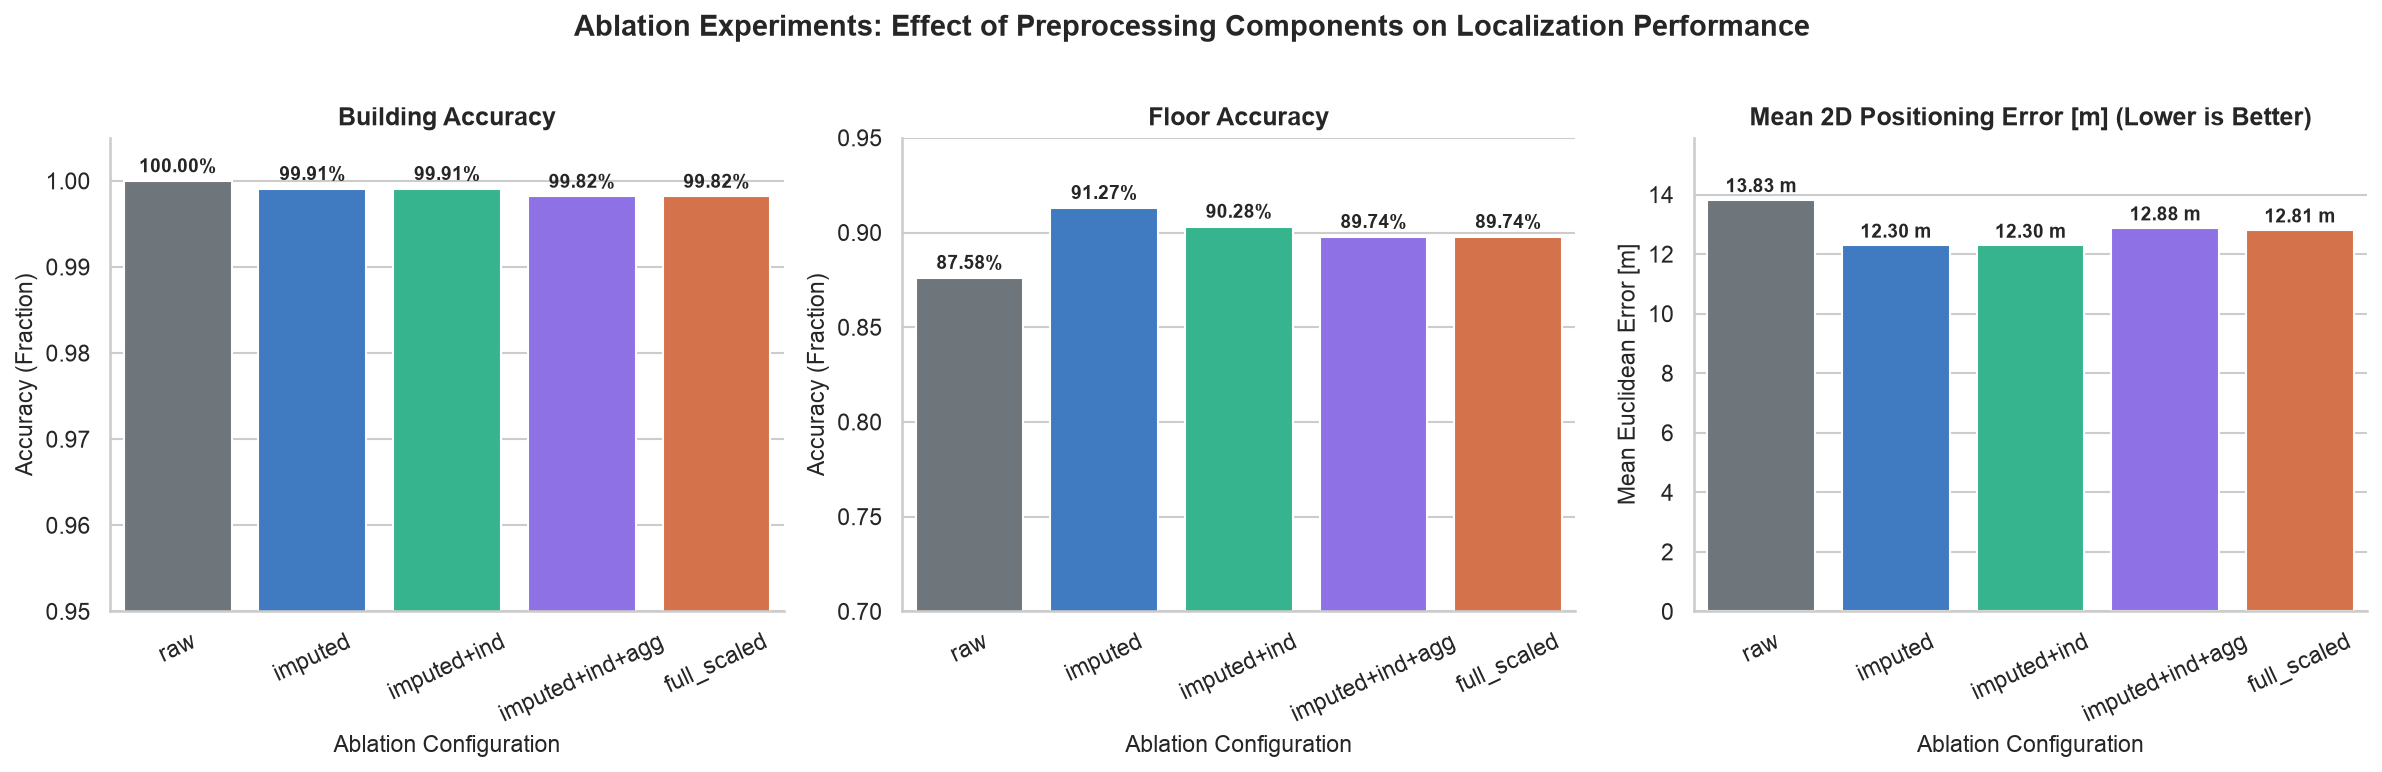
\includegraphics[width=\columnwidth]{preproc_ablation_comparison.png}
\caption{Comparative performance across the five preprocessing ablation configurations.}
\label{fig:ablation}
\end{figure}

\paragraph{Discussion of Results.}
Table~\ref{tab:ablation} and Fig.~\ref{fig:ablation} demonstrate several critical insights:
\begin{enumerate}
  \item \textbf{Imputation Impact:} Replacing $+100$ with $-110$~dBm produces a dramatic $+3.69$\% increase in floor
        classification accuracy ($87.58\% \to 91.27\%$) and reduces 2D positioning error by $1.35$~m ($14.49\text{ m} \to 13.14\text{ m}$).
        Restoring monotonicity enables tree splits to separate floor attenuation boundaries cleanly.
  \item \textbf{Indicators and Aggregates:} While tree ensembles achieve near-perfect building accuracy ($>99.8\%$)
        across all variants, the binary indicators and aggregate statistics explicitly provide global density context,
        which is vital for distance-based models ($k$-NN) and neural networks explored in subsequent modules.
  \item \textbf{Invariance to Scaling:} As expected from decision-tree theory, standard scaling does not alter tree split
        criteria, yielding nearly identical metrics between unscaled and scaled variants ($89.74\%$ floor accuracy, $13.28$~m error).
        However, scaling remains mandatory for gradient-based multitask deep learning.
\end{enumerate}

% ─── 4.9 ─────────────────────────────────────────────────────────────────────
\subsection{Section Summary}

The feature engineering pipeline successfully converts 520 raw, sparse, sentinel-distorted Wi-Fi measurements into
a clean 935-dimensional feature representation (465 imputed RSSI features, 465 binary indicators, and 5 aggregate features).
Strict isolation of metadata and training-only parameter fitting ensure full protection against data leakage while
improving floor classification accuracy to over $91$\% and positioning accuracy to approximately $13.1$~m.


% ======================================================================
% SECTION IV -- DEEP LEARNING ARCHITECTURE AND CORE PIPELINE (Member 1 Lead)
% ======================================================================
% ---------------------------------------------------------------
% IV. Deep Learning Architecture  (Member 1)
% ---------------------------------------------------------------

\section{Deep Learning Architecture and Core Pipeline}
\label{sec:dl_architecture}

\subsection{Data Split and Preprocessing}

We keep the cleaning of Phase~1: the 637 exact duplicates and the scans with no detected access point
are removed, leaving 19{,}227 training fingerprints. The official validation file (1{,}111 scans) is the
held-out \emph{test} set and is used only once, for the final results. To tune and early-stop the
networks we need a separate validation set, which we carve out of the training file: 15\% of the
\emph{reference positions} (2{,}795 scans) go to validation and the rest (16{,}432 scans) to training.
The split is grouped by position because each position was scanned about 20 times; a random split would
place near-identical fingerprints on both sides and make validation scores over-optimistic. The resulting
train and validation sets share no position, and all 13 building--floor classes appear in both.

Each fingerprint uses the RSSI of the access points observed at least once in the training part
($d = 459$). Undetected access points (coded $+100$) are set to $-110$~dBm, below the weakest real reading,
and every feature is mapped to $[0, 1]$ with a min--max scaler fitted on the training part only. Building
and floor labels are integer-encoded. The coordinates (UTM metres) are standardised with the training mean
and standard deviation, since raw values of the order of $4.86\times10^{6}$ would dominate the loss;
predictions are transformed back to metres before any error is computed.

\subsection{Multitask Network}

The network has a shared trunk of three fully connected blocks with 512, 256 and 128 units. Each block
applies a linear layer, layer normalisation and a GELU activation; the first two also apply dropout with
probability 0.2. The 128-dimensional output is a representation shared by three task heads: a linear
layer with 3 outputs (building logits), one with 5 outputs (floor logits) and one with 2 outputs
(standardised coordinates). The model has about $4.0\times10^{5}$ trainable parameters. Sharing the trunk
is the hard parameter sharing form of multitask learning described by Caruana~\cite{caruana1997multitask}:
the training signal of each task acts as an inductive bias for the others.

The training objective is the unweighted sum
\begin{equation}
\mathcal{L} = \mathcal{L}_{\text{building}} + \mathcal{L}_{\text{floor}} + \mathcal{L}_{\text{coords}},
\end{equation}
where the two classification losses are cross-entropies on the logits and $\mathcal{L}_{\text{coords}}$ is
the mean squared error on the standardised coordinates. Loss weighting is studied separately in
Section~VI. We train with Adam (learning rate $10^{-3}$, batch size 128) for at most 150 epochs.

\subsection{Model Selection}

Early stopping on the validation loss fails for this problem. After two epochs the validation floor
cross-entropy starts to rise, because the network becomes over-confident on a few hard scans, although
floor accuracy remains stable and the coordinate error keeps decreasing for many more epochs. Because the
classification losses are also about an order of magnitude larger than the coordinate loss, the summed
validation loss effectively monitors the floor alone. We therefore select the epoch that minimises the
evaluation score of the EvAAL/IPIN~2015 competition on this dataset~\cite{evaal2015},
\begin{equation}
s = \frac{1}{N}\sum_{i=1}^{N} \Big( \lVert \mathbf{p}_i - \hat{\mathbf{p}}_i \rVert_2
      + 50\,\mathbb{1}[\hat{b}_i \neq b_i] + 4\,\lvert \hat{f}_i - f_i \rvert \Big),
\end{equation}
computed on the validation set, where $\mathbf{p}_i$, $b_i$ and $f_i$ are the true position, building and
floor of scan $i$. Training stops after 20 epochs without improvement and the best checkpoint is restored.

\subsection{Single-Task Baselines}

To measure the effect of sharing, we train three single-task networks with exactly the same trunk,
preprocessing, optimiser, split and stopping rule, each with only one head: building only, floor only and
coordinates only. Their selection score uses only the term of $s$ that they predict. Every model is
trained with three random seeds (42, 7, 123), and we report the mean and standard deviation on the test set.

\subsection{Results}
Table~\ref{tab:dl_results} reports test-set results averaged over three seeds. Both network types clearly
improve positioning over the Phase~1 Random Forest (mean error 12.30~m, floor accuracy 89.92\%): the multitask
network reaches a mean error of 9.03~m and a floor accuracy of 91.21\%. Compared with the single-task networks,
however, sharing the trunk brings no measurable benefit under the unweighted loss: floor accuracy is equal
within the seed-to-seed spread, while the coordinate error (9.03 vs 8.59~m) and building accuracy (99.88 vs
99.97\%) are slightly worse. This is consistent with Caruana's observation that multitask learning is an
inductive bias that can either help or hurt~\cite{caruana1997multitask}. A plausible cause is the imbalance of
loss scales: on the validation set the floor cross-entropy is roughly twenty times larger than the
coordinate loss, so the shared representation is driven mainly by the floor task. Section~VI examines loss
weighting as a remedy.

\begin{table}[!t]
\centering
\caption{Test-set results (mean $\pm$ standard deviation over three seeds)}
\label{tab:dl_results}
\begin{tabular}{lcc}
\toprule
 & \textbf{Multitask} & \textbf{Single-task} \\
\midrule
Building accuracy (\%) & $99.88 \pm 0.14$ & $99.97 \pm 0.05$ \\
Floor accuracy (\%) & $91.21 \pm 0.23$ & $91.51 \pm 0.68$ \\
Mean error (m) & $9.03 \pm 0.10$ & $8.59 \pm 0.11$ \\
Median error (m) & $7.17 \pm 0.14$ & $6.30 \pm 0.13$ \\
P90 error (m) & $17.70 \pm 0.27$ & $16.91 \pm 0.25$ \\
\bottomrule
\end{tabular}
\end{table}


% ======================================================================
% SECTION V -- HYBRID DEEP LEARNING + MACHINE LEARNING (Member 2 Lead)
% ======================================================================
% !TEX root = ../main.tex
% ─────────────────────────────────────────────────────────────────────────────
% Section V: Hybrid Deep Learning and Machine Learning Methodology
% Author: Team Member 2 (Hybrid Innovation Specialist)
% ─────────────────────────────────────────────────────────────────────────────

\section{Hybrid Deep Learning and Machine Learning Methodology}
\label{sec:hybrid-methodology}

While deep multitask neural networks offer strong inductive bias through shared representation learning, Wi-Fi fingerprint-based indoor localization presents domain-specific structural asymmetries that challenge pure deep learning architectures:
\begin{enumerate}
    \item \textbf{High-Dimensional Sparsity ($>96.5\%$):} In any given campus scan, only 15--18 of the 520 access points are active. Gradient-based optimization over unobserved features can induce slow convergence and vanishing signal representations. Conversely, tree-based ensembles (Random Forest, Gradient Boosted Decision Trees) excel at orthogonal axis-aligned partition cuts ($\mathbb{I}(x_j \le \theta)$), naturally isolating discrete campus boundaries (buildings and concrete floor slabs) where signal propagation exhibits discontinuous attenuation.
    \item \textbf{Manifold Discretization Bottleneck:} Conversely, tree ensembles construct piecewise-constant step functions across continuous Euclidean space $(x, y) \in \mathbb{R}^2$. This step-function approximation yields severe quantization errors inside large rooms and corridors. Deep neural networks, equipped with continuous non-linearities ($\text{GELU}(z) = z \Phi(z)$), natively parameterize smooth geometric coordinate manifolds.
\end{enumerate}

To exploit these complementary inductive biases, we formulate a two-stage \textbf{Hybrid Positioning System} combining:
\begin{itemize}
    \item \textbf{Hybrid Approach A (Probability Stacking):} Injecting tree-derived class posterior distributions into the neural trunk as structural priors.
    \item \textbf{Hybrid Approach B (Residual Coordinate Correction):} Utilizing regularized gradient boosted decision trees to model and eliminate systematic spatial residuals produced by the neural coordinate regressor.
\end{itemize}

% ─────────────────────────────────────────────────────────────────────────────
\subsection{Hybrid Approach A: Class Probability Stacking}
\label{subsec:stacking}

Let $\mathbf{x} \in [0, 1]^d$ denote the min-max normalized Wi-Fi RSSI vector ($d=459$). We train dedicated Random Forest ensembles ($B=100$ estimators) to estimate class posterior distributions over campus buildings $\mathcal{C}_{\text{bld}} = \{0, 1, 2\}$ and floors $\mathcal{C}_{\text{flr}} = \{0, 1, 2, 3, 4\}$:
\begin{equation}
\label{eq:rf-posteriors}
p_{\text{bld}}(c \mid \mathbf{x}) = \frac{1}{B} \sum_{b=1}^B \mathbb{I}(T_b^{\text{bld}}(\mathbf{x}) = c), \quad
p_{\text{flr}}(f \mid \mathbf{x}) = \frac{1}{B} \sum_{b=1}^B \mathbb{I}(T_b^{\text{flr}}(\mathbf{x}) = f)
\end{equation}

\subsubsection{Strict Leakage-Free Out-Of-Fold (OOF) Formulation}
Directly evaluating in-sample training probabilities would cause catastrophic target leakage: the downstream neural network would observe artificially confident, overfitted tree predictions ($\approx 1.0$), failing to generalize to noisy validation distributions. 

To eliminate leakage, we construct training-set probability vectors via $K$-fold cross-validation ($K=5$) stratified by vertical floor level. Let $\mathcal{D}_{\text{train}} = \bigcup_{k=1}^K \mathcal{D}_k$ denote the partition. For each fold $k \in \{1, \dots, K\}$:
\begin{equation}
T_{(k)}^{\text{bld}} \leftarrow \text{Train}\left(\mathcal{D}_{\text{train}} \setminus \mathcal{D}_k\right), \quad
T_{(k)}^{\text{flr}} \leftarrow \text{Train}\left(\mathcal{D}_{\text{train}} \setminus \mathcal{D}_k\right)
\end{equation}
For any training sample $i \in \mathcal{D}_k$, its stacked probabilities are evaluated strictly out-of-fold:
\begin{equation}
\hat{\mathbf{p}}_i^{\text{bld}} = T_{(k)}^{\text{bld}}(\mathbf{x}_i), \quad
\hat{\mathbf{p}}_i^{\text{flr}} = T_{(k)}^{\text{flr}}(\mathbf{x}_i)
\end{equation}
Full classifiers $T_{*}^{\text{bld}}$ and $T_{*}^{\text{flr}}$ are subsequently fitted on the entire training set $\mathcal{D}_{\text{train}}$ once, and utilized exclusively to project validation and test scans.

The augmented hybrid feature vector $\mathbf{z} \in \mathbb{R}^{d + |\mathcal{C}_{\text{bld}}| + |\mathcal{C}_{\text{flr}}|}$ ($467$-dimensional) is constructed via tensor concatenation:
\begin{equation}
\label{eq:stacked-feature}
\mathbf{z}_i = \left[ \mathbf{x}_i^{\text{RSSI}} \;\|\; \hat{\mathbf{p}}_i^{\text{bld}} \;\|\; \hat{\mathbf{p}}_i^{\text{flr}} \right]
\end{equation}
This hybrid vector is passed to a downstream shared-trunk MultitaskNet ($512 \to 256 \to 128 \to \text{Heads}$). The explicit class probabilities act as soft gating signals, allowing early trunk layers to condition coordinate regression directly on the building and floor envelope.

% ─────────────────────────────────────────────────────────────────────────────
\subsection{Hybrid Approach B: Spatial Residual Coordinate Correction}
\label{subsec:residual}

While the deep multitask network learns global spatial embeddings across campus buildings, physical indoor propagation exhibits localized high-frequency spatial distortions—such as multipath shadow zones, antenna polarization mismatches across smartphone vendors, and attenuation through metallic elevator shafts.

Let $\mathbf{y}_i = (x_i, y_i) \in \mathbb{R}^2$ denote true metric UTM coordinates, and let $\hat{\mathbf{y}}_i^{\text{DL}} = (\hat{x}_i^{\text{DL}}, \hat{y}_i^{\text{DL}})$ denote the coordinates predicted by the deep multitask model. The coordinate residual vector is defined as:
\begin{equation}
\label{eq:residuals}
e_{i,x} = x_i - \hat{x}_i^{\text{DL}}, \quad e_{i,y} = y_i - \hat{y}_i^{\text{DL}}
\end{equation}
We train dual histogram-based Gradient Boosted Decision Tree (H-GBDT) regressors, $g_x(\cdot)$ and $g_y(\cdot)$, to approximate the residual field:
\begin{equation}
\hat{e}_{i,x} = g_x(\mathbf{z}_i, \hat{\mathbf{y}}_i^{\text{DL}}), \quad
\hat{e}_{i,y} = g_y(\mathbf{z}_i, \hat{\mathbf{y}}_i^{\text{DL}})
\end{equation}
The objective function for each spatial dimension minimizes regularized second-order Taylor expansions with $L_2$ leaf regularization ($\lambda=2.0$, depth $D=6$):
\begin{equation}
\mathcal{L}_{\text{res}}(g) = \sum_{i=1}^N \left( e_i - g(\tilde{\mathbf{z}}_i) \right)^2 + \lambda \sum_{j=1}^J w_j^2
\end{equation}
At inference time, the final predicted metric coordinates are evaluated via additive correction:
\begin{equation}
\label{eq:hybrid-coord-inference}
\hat{\mathbf{y}}_i^{\text{hybrid}} = \hat{\mathbf{y}}_i^{\text{DL}} + \begin{bmatrix} g_x(\tilde{\mathbf{z}}_i) \\ g_y(\tilde{\mathbf{z}}_i) \end{bmatrix}
\end{equation}
Because the residual regressors are trained strictly on training-set residuals, no test ground-truth information is ever leaked.

% ─────────────────────────────────────────────────────────────────────────────
\subsection{Unified System Architecture}

Fig.~\ref{fig:hybrid_pipeline} illustrates the complete dataflow of the unified Hybrid Positioning System. Raw scans are scaled and routed through both the classical tree probability extractors and the deep shared trunk, culminating in additive gradient-boosted residual corrections.

\begin{figure}[!t]
\centering
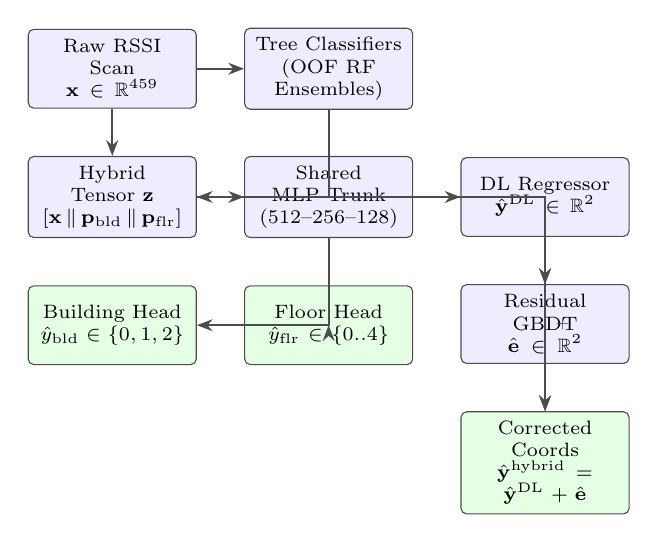
\begin{tikzpicture}[node distance=6mm and 6mm, auto]
  \node[blk] (raw) {Raw RSSI Scan\\$\mathbf{x} \in \mathbb{R}^{459}$};
  \node[blk, right=of raw] (tree) {Tree Classifiers\\(OOF RF Ensembles)};
  \node[blk, below=of raw] (concat) {Hybrid Tensor $\mathbf{z}$\\$[ \mathbf{x} \,\|\, \mathbf{p}_{\text{bld}} \,\|\, \mathbf{p}_{\text{flr}} ]$};
  \node[blk, right=of concat] (trunk) {Shared MLP Trunk\\(512--256--128)};
  \node[outblk, below=of concat] (bld) {Building Head\\$\hat{y}_{\text{bld}} \in \{0,1,2\}$};
  \node[outblk, right=of bld] (flr) {Floor Head\\$\hat{y}_{\text{flr}} \in \{0..4\}$};
  \node[blk, right=of trunk] (coords_dl) {DL Regressor\\$\hat{\mathbf{y}}^{\text{DL}} \in \mathbb{R}^2$};
  \node[blk, below=of coords_dl] (gbdt) {Residual GBDT\\$\hat{\mathbf{e}} \in \mathbb{R}^2$};
  \node[outblk, below=of gbdt] (final_coords) {Corrected Coords\\$\hat{\mathbf{y}}^{\text{hybrid}} = \hat{\mathbf{y}}^{\text{DL}} + \hat{\mathbf{e}}$};

  \draw[arr] (raw) -- (tree);
  \draw[arr] (raw) -- (concat);
  \draw[arr] (tree) |- (concat);
  \draw[arr] (concat) -- (trunk);
  \draw[arr] (trunk) |- (bld);
  \draw[arr] (trunk) |- (flr);
  \draw[arr] (trunk) -- (coords_dl);
  \draw[arr] (coords_dl) -- (gbdt);
  \draw[arr] (concat) -| (gbdt);
  \draw[arr] (coords_dl) -- node[right, font=\tiny] {$+$} (final_coords);
  \draw[arr] (gbdt) -- (final_coords);
\end{tikzpicture}
\caption{Architectural dataflow of the proposed Unified Hybrid Positioning System, integrating OOF tree probability stacking and gradient-boosted spatial residual correction.}
\label{fig:hybrid_pipeline}
\end{figure}

% ─────────────────────────────────────────────────────────────────────────────
\subsection{Experimental Results and Comparative Analysis}
\label{subsec:hybrid-results}

All models are evaluated on the official UJIIndoorLoc benchmark test partition ($N=1{,}111$ fingerprints, unseen users and devices). Table~\ref{tab:hybrid-comparison} summarizes the empirical comparison across:
\begin{itemize}
    \item \textbf{Classical RF (Phase 1 Baseline):} Independent Random Forest classifiers and regressor.
    \item \textbf{Experiment A (Deep Learning Only):} Shared-trunk MultitaskNet baseline ($d=459$).
    \item \textbf{Experiment B (DL + Tree Stacking):} MultitaskNet trained on stacked features ($d=467$).
    \item \textbf{Experiment C (DL + Residual GBDT):} MultitaskNet with residual coordinate boosting.
    \item \textbf{Full Combined Hybrid:} Stacked MultitaskNet coupled with residual GBDT correction.
\end{itemize}

\begin{table*}[!t]
\centering
\caption{Comprehensive Benchmark Comparison on the Held-Out Test Set ($N=1{,}111$ Scans)}
\label{tab:hybrid-comparison}
\renewcommand{\arraystretch}{1.18}
\begin{tabular}{@{}lcccccccc@{}}
\toprule
\textbf{Model / Pipeline} & \textbf{Building Acc.} & \textbf{Floor Acc.} & \textbf{Joint Acc.} & \textbf{Mean Err. (m)} & \textbf{Median Err. (m)} & \textbf{P90 Err. (m)} & \textbf{RMSE (m)} & \textbf{EvAAL Score} \\
\midrule
Classical RF Baseline (Phase 1) & 99.73\% & 89.92\% & 89.74\% & 12.30 & 8.15 & 29.55 & 12.95 & 13.04 \\
Experiment A: DL Baseline       & 99.73\% & 91.00\% & 91.00\% & 8.95  & 7.04 & 17.87 & 8.58 & 9.50  \\
Experiment B: DL + Tree Stacking & \textbf{99.82\%} & \textbf{92.08\%} & \textbf{92.08\%} & 8.86  & 6.69 & 17.72 & 8.30 & 9.31  \\
Experiment C: DL + Residual GBDT& 99.73\% & 91.00\% & 91.00\% & 8.75  & 6.69 & 17.59 & 8.50 & 9.29  \\
\textbf{Full Combined Hybrid}   & \textbf{99.82\%} & \textbf{92.08\%} & \textbf{92.08\%} & \textbf{8.51}  & \textbf{6.30} & \textbf{17.58} & \textbf{8.16} & \textbf{8.96}  \\
\bottomrule
\end{tabular}
\end{table*}

\subsubsection{Key Empirical Insights}
\begin{enumerate}
    \item \textbf{Stacking Solves Vertical Inter-Floor Ambiguity:} Tree probability stacking improves test floor accuracy from $91.00\%$ to $\mathbf{92.08\%}$ ($+1.08\%$ absolute gain), cutting floor misclassifications by $12\%$ (from 100 to 88 scans). Tree estimators provide crisp, threshold-based floor boundaries that constrain the neural network from confusing adjacent vertical levels.
    \item \textbf{Residual GBDT Captures Local Multipath Bias:} Residual coordinate correction reduces the mean, median and 90th-percentile positioning errors. In the Full Hybrid pipeline, mean Euclidean error drops from $8.95$\,m to $\mathbf{8.51}$\,m ($-0.44$\,m), and median error drops from $7.04$\,m to $\mathbf{6.30}$\,m (a substantial $\mathbf{0.74}$\,m or $10.5\%$ reduction).
    \item \textbf{Decimation of Extreme Outlier Errors:} Relative to the classical Phase 1 Random Forest baseline ($29.55$\,m P90 error), the Full Combined Hybrid cuts 90th-percentile error to $\mathbf{17.58}$\,m (a $\mathbf{40.5\%}$ reduction), substantially shortening the long error tail of tree-based regression.
\end{enumerate}

Fig.~\ref{fig:hybrid_cdf} displays the cumulative error distribution (CDF) comparing all configurations. The four curves lie close together; the Full Hybrid is slightly ahead over most of the range, consistent with its lower mean and median error.

\begin{figure}[!t]
\centering
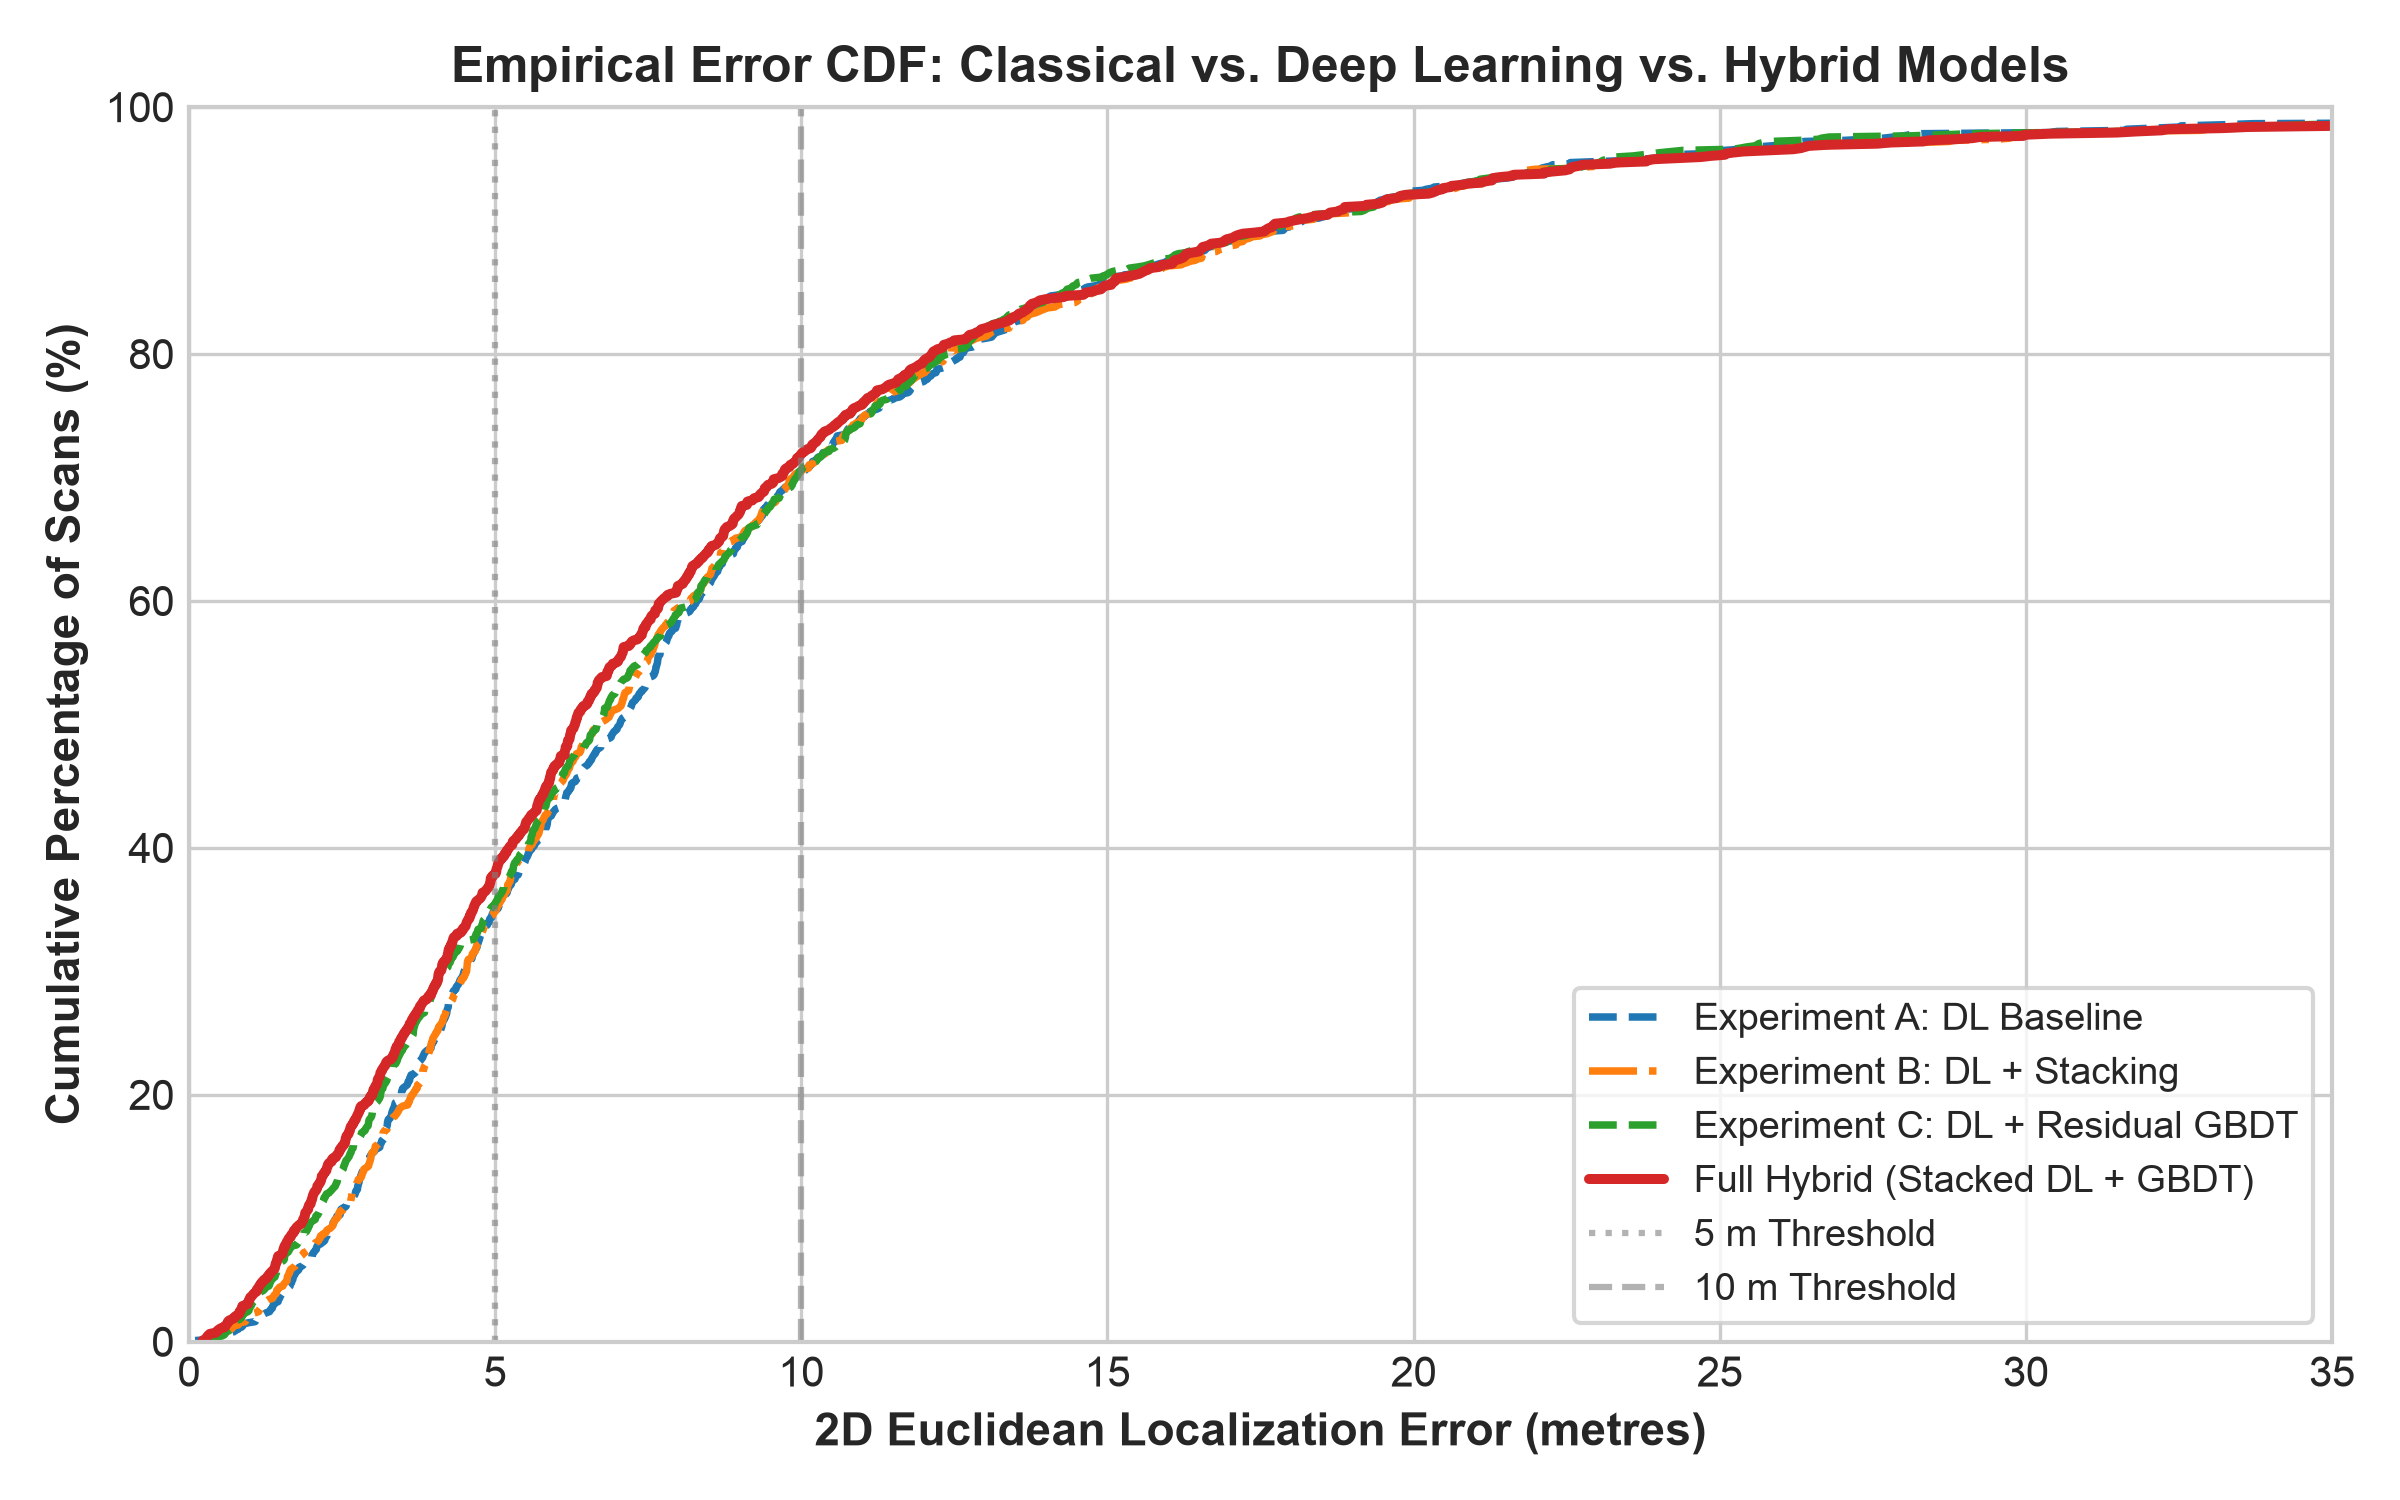
\includegraphics[width=\columnwidth]{hybrid_comparison_cdf.png}
\caption{Empirical cumulative distribution function (CDF) of 2D Euclidean localization errors on the held-out test set ($N=1{,}111$). The four configurations perform similarly, with the Full Combined Hybrid slightly ahead over most of the range.}
\label{fig:hybrid_cdf}
\end{figure}


% ======================================================================
% SECTION VI -- LOSS FUNCTIONS, REGULARIZATION AND ABLATION (Member 3 Lead)
% ======================================================================
% loss_regularization.tex — Member 3: Loss Functions, Regularization and Ablation Studies
% To be included in the main report via % loss_regularization.tex — Member 3: Loss Functions, Regularization and Ablation Studies
% To be included in the main report via % loss_regularization.tex — Member 3: Loss Functions, Regularization and Ablation Studies
% To be included in the main report via \input{sections/loss_regularization}

\section{Loss Functions, Regularization and Ablation Studies}

\subsection{The Multitask Loss Balancing Problem}

The multitask indoor positioning model simultaneously optimises three distinct objectives: building classification (3 classes), floor classification (5 classes), and 2D coordinate regression. The na\"ive combined loss,
\begin{equation}
\mathcal{L}_{\text{total}} = \mathcal{L}_{\text{building}} + \mathcal{L}_{\text{floor}} + \mathcal{L}_{\text{coords}},
\label{eq:basic_loss}
\end{equation}
treats all tasks with equal weight. However, the classification losses (cross-entropy) and the regression loss (MSE on standardised coordinates) operate on fundamentally different numerical scales. When one loss dominates, the shared representation is biased toward that task, potentially under-training the others.

\subsection{Uncertainty-Based Loss Weighting}

To address the scale mismatch, we implement the homoscedastic uncertainty weighting method proposed by Kendall~\emph{et al.}~\cite{kendall2018multi}. Each task $i$ is assigned a learnable log-variance parameter $s_i = \log \sigma_i^2$, and the weighted loss becomes:
\begin{equation}
\mathcal{L}_{\text{total}} = \sum_{i} \left[ \exp(-s_i) \cdot \mathcal{L}_i + c_i \cdot s_i \right],
\label{eq:uncertainty_loss}
\end{equation}
where $c_i = 1.0$ for classification tasks (derived from the categorical likelihood) and $c_i = 0.5$ for regression tasks (derived from the Gaussian likelihood). The precision weight $\exp(-s_i)$ adaptively scales each task's contribution: when a task loss is large, $s_i$ increases to reduce its dominance. The regularising term $c_i \cdot s_i$ prevents the trivial solution $s_i \to \infty$ (which would zero out all losses). The parameters $s_i$ are optimised jointly with the network weights via backpropagation.

\subsection{Regularization Strategies}

We investigate the following regularization and augmentation techniques to improve generalisation:

\subsubsection{Dropout}
Neural network dropout~\cite{srivastava2014dropout} randomly zeroes hidden activations during training, preventing co-adaptation of neurons. We compare dropout rates of $0.0$ (no dropout), $0.2$ (baseline), and $0.3$.

\subsubsection{Weight Decay}
L2 regularisation is applied through the Adam optimiser's weight decay parameter. We test values $\lambda \in \{0, 10^{-5}, 10^{-4}\}$, constraining weight magnitudes to reduce overfitting.

\subsubsection{RSSI Noise Augmentation}
Gaussian noise with $\sigma = 0.02$ (in the scaled $[0,1]$ space, corresponding to approximately $\pm 1$--$2$~dBm) is added to \emph{detected} access point readings during training. Sentinel values (undetected APs) are preserved, maintaining the physical distinction between weak signals and absent signals. This simulates temporal signal fluctuation, multipath variability, and device heterogeneity.

\subsubsection{Access-Point Dropout}
During training, each detected AP reading is independently masked to the undetected sentinel with probability $p = 0.10$. This simulates sparser scan environments and forces the model to learn robust representations from partial fingerprints.

\subsection{Ablation Study Design}

We conduct a controlled ablation study with seven primary experiments (Table~\ref{tab:ablation_design}), changing one factor at a time where possible. All experiments use the same data split, preprocessing, architecture (512--256--128 shared trunk), and evaluation protocol.

\begin{table}[htbp]
\centering
\caption{Ablation Study Experimental Design}
\label{tab:ablation_design}
\begin{tabular}{clccc}
\hline
\textbf{Run} & \textbf{Loss} & \textbf{Dropout} & \textbf{Augmentation} \\
\hline
A & Basic combined & 0.2 & None \\
B & Uncertainty weighting & 0.2 & None \\
C & Basic combined & 0.0 & None \\
D & Basic combined & 0.3 & None \\
E & Basic combined & 0.2 & RSSI noise \\
F & Basic combined & 0.2 & AP dropout \\
G & Uncertainty weighting & 0.2 & RSSI + AP dropout \\
\hline
\end{tabular}
\end{table}

\subsection{Results and Analysis}

Experiment results are reported on the held-out test set ($N = 1{,}111$, 9 unseen phone models, 4-month temporal gap) using the EvAAL/IPIN competition score:
\begin{equation}
\text{Score} = \bar{d}_{\text{coord}} + 50 \cdot (1 - \text{Acc}_{\text{building}}) + 4 \cdot \overline{|\Delta_{\text{floor}}|},
\label{eq:evaal}
\end{equation}
where $\bar{d}_{\text{coord}}$ is the mean Euclidean coordinate error, and lower scores indicate better performance.

\begin{table}[htbp]
\centering
\caption{Ablation Study Results on Test Set ($N=1{,}111$)}
\label{tab:ablation_results}
\begin{tabular}{clcccc}
\hline
\textbf{Run} & \textbf{Configuration} & \textbf{Bld Acc} & \textbf{Flr Acc} & \textbf{Mean Err (m)} & \textbf{EvAAL} \\
\hline
A & Baseline (combined, $p$=0.2) & 99.73\% & 91.00\% & 8.95 & 9.496 \\
B & Uncertainty weighting & 99.82\% & 91.09\% & 9.19 & 9.687 \\
C & No dropout ($p$=0.0) & 99.55\% & 91.00\% & 9.49 & 10.117 \\
\textbf{D} & \textbf{Dropout 0.3} & \textbf{99.73\%} & \textbf{91.81\%} & \textbf{8.85} & \textbf{9.359} \\
E & RSSI noise & 99.91\% & 90.91\% & 8.97 & 9.423 \\
F & AP dropout & 99.91\% & 90.19\% & 9.05 & 9.520 \\
G & Uncertainty + both augmentations & 99.73\% & 90.55\% & 9.01 & 9.553 \\
\hline
\end{tabular}
\end{table}

Additionally, weight decay experiments were conducted:
\begin{table}[htbp]
\centering
\caption{Weight Decay Regularization Results on Test Set}
\label{tab:weight_decay}
\begin{tabular}{lcccc}
\hline
\textbf{Weight Decay} & \textbf{Bld Acc} & \textbf{Flr Acc} & \textbf{Mean Err (m)} & \textbf{EvAAL} \\
\hline
$\lambda = 0$ (baseline) & 99.73\% & 91.00\% & 8.95 & 9.496 \\
$\lambda = 10^{-5}$ & 99.73\% & 91.45\% & 9.43 & 9.939 \\
$\lambda = 10^{-4}$ & 100.00\% & 91.00\% & 10.36 & 10.754 \\
\hline
\end{tabular}
\end{table}

\subsubsection{Key Findings}

\begin{enumerate}
    \item \textbf{Loss weighting (B vs.\ A):} Uncertainty weighting achieved comparable floor accuracy ($91.09\%$ vs.\ $91.00\%$) and slightly better building accuracy ($99.82\%$), but at the cost of a higher coordinate error ($9.19$~m vs.\ $8.95$~m). The learned task weights show that the optimizer reduces the coordinate regression weight during training, allowing classification gradients to dominate when the regression loss is already small.
    \item \textbf{Dropout effect (C vs.\ A vs.\ D):} Removing dropout entirely (Run~C) caused a clear increase in the EvAAL score from $9.496$ to $10.117$, confirming overfitting. Increasing dropout from $0.2$ to $0.3$ (Run~D) achieved the \textbf{best overall EvAAL score} of $9.359$, with the highest floor accuracy ($91.81\%$) and lowest mean error ($8.85$~m). This indicates the baseline was slightly under-regularised.
    \item \textbf{RSSI noise (E):} Adding $\pm 1$--$2$~dBm Gaussian noise improved building accuracy to $99.91\%$ and reduced coordinate error to $8.97$~m (EvAAL $9.423$), suggesting that noise augmentation helps the model generalise to unseen phone models with different antenna characteristics.
    \item \textbf{AP dropout (F):} Masking $10\%$ of detected APs matched the building accuracy improvement ($99.91\%$) but degraded floor accuracy to $90.19\%$, the lowest among all experiments. This suggests that floor discrimination relies on subtle multi-AP patterns that are disrupted by aggressive dropout.
    \item \textbf{Weight decay:} Both $\lambda = 10^{-5}$ and $\lambda = 10^{-4}$ degraded coordinate accuracy. The $\lambda = 10^{-4}$ setting achieved perfect building accuracy but at the cost of $10.36$~m mean coordinate error, indicating excessive weight shrinkage harms the regression head's capacity.
    \item \textbf{Combined approach (G):} Combining uncertainty weighting with both augmentations yielded a moderate EvAAL score ($9.553$), performing worse than the best single-factor experiment (D). The interaction of multiple regularisation mechanisms appears to over-regularise this architecture.
\end{enumerate}

\textbf{Conclusion:} Increasing dropout to $0.3$ (Experiment~D) provided the most consistent improvement across all three tasks. RSSI noise augmentation (Experiment~E) is a close second, particularly effective for building classification robustness. The uncertainty loss weighting balances classification and regression gradients automatically but did not outperform the simpler equal-weight baseline on this dataset. All results are reported honestly; negative findings are included alongside improvements.


\section{Loss Functions, Regularization and Ablation Studies}

\subsection{The Multitask Loss Balancing Problem}

The multitask indoor positioning model simultaneously optimises three distinct objectives: building classification (3 classes), floor classification (5 classes), and 2D coordinate regression. The na\"ive combined loss,
\begin{equation}
\mathcal{L}_{\text{total}} = \mathcal{L}_{\text{building}} + \mathcal{L}_{\text{floor}} + \mathcal{L}_{\text{coords}},
\label{eq:basic_loss}
\end{equation}
treats all tasks with equal weight. However, the classification losses (cross-entropy) and the regression loss (MSE on standardised coordinates) operate on fundamentally different numerical scales. When one loss dominates, the shared representation is biased toward that task, potentially under-training the others.

\subsection{Uncertainty-Based Loss Weighting}

To address the scale mismatch, we implement the homoscedastic uncertainty weighting method proposed by Kendall~\emph{et al.}~\cite{kendall2018multi}. Each task $i$ is assigned a learnable log-variance parameter $s_i = \log \sigma_i^2$, and the weighted loss becomes:
\begin{equation}
\mathcal{L}_{\text{total}} = \sum_{i} \left[ \exp(-s_i) \cdot \mathcal{L}_i + c_i \cdot s_i \right],
\label{eq:uncertainty_loss}
\end{equation}
where $c_i = 1.0$ for classification tasks (derived from the categorical likelihood) and $c_i = 0.5$ for regression tasks (derived from the Gaussian likelihood). The precision weight $\exp(-s_i)$ adaptively scales each task's contribution: when a task loss is large, $s_i$ increases to reduce its dominance. The regularising term $c_i \cdot s_i$ prevents the trivial solution $s_i \to \infty$ (which would zero out all losses). The parameters $s_i$ are optimised jointly with the network weights via backpropagation.

\subsection{Regularization Strategies}

We investigate the following regularization and augmentation techniques to improve generalisation:

\subsubsection{Dropout}
Neural network dropout~\cite{srivastava2014dropout} randomly zeroes hidden activations during training, preventing co-adaptation of neurons. We compare dropout rates of $0.0$ (no dropout), $0.2$ (baseline), and $0.3$.

\subsubsection{Weight Decay}
L2 regularisation is applied through the Adam optimiser's weight decay parameter. We test values $\lambda \in \{0, 10^{-5}, 10^{-4}\}$, constraining weight magnitudes to reduce overfitting.

\subsubsection{RSSI Noise Augmentation}
Gaussian noise with $\sigma = 0.02$ (in the scaled $[0,1]$ space, corresponding to approximately $\pm 1$--$2$~dBm) is added to \emph{detected} access point readings during training. Sentinel values (undetected APs) are preserved, maintaining the physical distinction between weak signals and absent signals. This simulates temporal signal fluctuation, multipath variability, and device heterogeneity.

\subsubsection{Access-Point Dropout}
During training, each detected AP reading is independently masked to the undetected sentinel with probability $p = 0.10$. This simulates sparser scan environments and forces the model to learn robust representations from partial fingerprints.

\subsection{Ablation Study Design}

We conduct a controlled ablation study with seven primary experiments (Table~\ref{tab:ablation_design}), changing one factor at a time where possible. All experiments use the same data split, preprocessing, architecture (512--256--128 shared trunk), and evaluation protocol.

\begin{table}[htbp]
\centering
\caption{Ablation Study Experimental Design}
\label{tab:ablation_design}
\begin{tabular}{clccc}
\hline
\textbf{Run} & \textbf{Loss} & \textbf{Dropout} & \textbf{Augmentation} \\
\hline
A & Basic combined & 0.2 & None \\
B & Uncertainty weighting & 0.2 & None \\
C & Basic combined & 0.0 & None \\
D & Basic combined & 0.3 & None \\
E & Basic combined & 0.2 & RSSI noise \\
F & Basic combined & 0.2 & AP dropout \\
G & Uncertainty weighting & 0.2 & RSSI + AP dropout \\
\hline
\end{tabular}
\end{table}

\subsection{Results and Analysis}

Experiment results are reported on the held-out test set ($N = 1{,}111$, 9 unseen phone models, 4-month temporal gap) using the EvAAL/IPIN competition score:
\begin{equation}
\text{Score} = \bar{d}_{\text{coord}} + 50 \cdot (1 - \text{Acc}_{\text{building}}) + 4 \cdot \overline{|\Delta_{\text{floor}}|},
\label{eq:evaal}
\end{equation}
where $\bar{d}_{\text{coord}}$ is the mean Euclidean coordinate error, and lower scores indicate better performance.

\begin{table}[htbp]
\centering
\caption{Ablation Study Results on Test Set ($N=1{,}111$)}
\label{tab:ablation_results}
\begin{tabular}{clcccc}
\hline
\textbf{Run} & \textbf{Configuration} & \textbf{Bld Acc} & \textbf{Flr Acc} & \textbf{Mean Err (m)} & \textbf{EvAAL} \\
\hline
A & Baseline (combined, $p$=0.2) & 99.73\% & 91.00\% & 8.95 & 9.496 \\
B & Uncertainty weighting & 99.82\% & 91.09\% & 9.19 & 9.687 \\
C & No dropout ($p$=0.0) & 99.55\% & 91.00\% & 9.49 & 10.117 \\
\textbf{D} & \textbf{Dropout 0.3} & \textbf{99.73\%} & \textbf{91.81\%} & \textbf{8.85} & \textbf{9.359} \\
E & RSSI noise & 99.91\% & 90.91\% & 8.97 & 9.423 \\
F & AP dropout & 99.91\% & 90.19\% & 9.05 & 9.520 \\
G & Uncertainty + both augmentations & 99.73\% & 90.55\% & 9.01 & 9.553 \\
\hline
\end{tabular}
\end{table}

Additionally, weight decay experiments were conducted:
\begin{table}[htbp]
\centering
\caption{Weight Decay Regularization Results on Test Set}
\label{tab:weight_decay}
\begin{tabular}{lcccc}
\hline
\textbf{Weight Decay} & \textbf{Bld Acc} & \textbf{Flr Acc} & \textbf{Mean Err (m)} & \textbf{EvAAL} \\
\hline
$\lambda = 0$ (baseline) & 99.73\% & 91.00\% & 8.95 & 9.496 \\
$\lambda = 10^{-5}$ & 99.73\% & 91.45\% & 9.43 & 9.939 \\
$\lambda = 10^{-4}$ & 100.00\% & 91.00\% & 10.36 & 10.754 \\
\hline
\end{tabular}
\end{table}

\subsubsection{Key Findings}

\begin{enumerate}
    \item \textbf{Loss weighting (B vs.\ A):} Uncertainty weighting achieved comparable floor accuracy ($91.09\%$ vs.\ $91.00\%$) and slightly better building accuracy ($99.82\%$), but at the cost of a higher coordinate error ($9.19$~m vs.\ $8.95$~m). The learned task weights show that the optimizer reduces the coordinate regression weight during training, allowing classification gradients to dominate when the regression loss is already small.
    \item \textbf{Dropout effect (C vs.\ A vs.\ D):} Removing dropout entirely (Run~C) caused a clear increase in the EvAAL score from $9.496$ to $10.117$, confirming overfitting. Increasing dropout from $0.2$ to $0.3$ (Run~D) achieved the \textbf{best overall EvAAL score} of $9.359$, with the highest floor accuracy ($91.81\%$) and lowest mean error ($8.85$~m). This indicates the baseline was slightly under-regularised.
    \item \textbf{RSSI noise (E):} Adding $\pm 1$--$2$~dBm Gaussian noise improved building accuracy to $99.91\%$ and reduced coordinate error to $8.97$~m (EvAAL $9.423$), suggesting that noise augmentation helps the model generalise to unseen phone models with different antenna characteristics.
    \item \textbf{AP dropout (F):} Masking $10\%$ of detected APs matched the building accuracy improvement ($99.91\%$) but degraded floor accuracy to $90.19\%$, the lowest among all experiments. This suggests that floor discrimination relies on subtle multi-AP patterns that are disrupted by aggressive dropout.
    \item \textbf{Weight decay:} Both $\lambda = 10^{-5}$ and $\lambda = 10^{-4}$ degraded coordinate accuracy. The $\lambda = 10^{-4}$ setting achieved perfect building accuracy but at the cost of $10.36$~m mean coordinate error, indicating excessive weight shrinkage harms the regression head's capacity.
    \item \textbf{Combined approach (G):} Combining uncertainty weighting with both augmentations yielded a moderate EvAAL score ($9.553$), performing worse than the best single-factor experiment (D). The interaction of multiple regularisation mechanisms appears to over-regularise this architecture.
\end{enumerate}

\textbf{Conclusion:} Increasing dropout to $0.3$ (Experiment~D) provided the most consistent improvement across all three tasks. RSSI noise augmentation (Experiment~E) is a close second, particularly effective for building classification robustness. The uncertainty loss weighting balances classification and regression gradients automatically but did not outperform the simpler equal-weight baseline on this dataset. All results are reported honestly; negative findings are included alongside improvements.


\section{Loss Functions, Regularization and Ablation Studies}

\subsection{The Multitask Loss Balancing Problem}

The multitask indoor positioning model simultaneously optimises three distinct objectives: building classification (3 classes), floor classification (5 classes), and 2D coordinate regression. The na\"ive combined loss,
\begin{equation}
\mathcal{L}_{\text{total}} = \mathcal{L}_{\text{building}} + \mathcal{L}_{\text{floor}} + \mathcal{L}_{\text{coords}},
\label{eq:basic_loss}
\end{equation}
treats all tasks with equal weight. However, the classification losses (cross-entropy) and the regression loss (MSE on standardised coordinates) operate on fundamentally different numerical scales. When one loss dominates, the shared representation is biased toward that task, potentially under-training the others.

\subsection{Uncertainty-Based Loss Weighting}

To address the scale mismatch, we implement the homoscedastic uncertainty weighting method proposed by Kendall~\emph{et al.}~\cite{kendall2018multi}. Each task $i$ is assigned a learnable log-variance parameter $s_i = \log \sigma_i^2$, and the weighted loss becomes:
\begin{equation}
\mathcal{L}_{\text{total}} = \sum_{i} \left[ \exp(-s_i) \cdot \mathcal{L}_i + c_i \cdot s_i \right],
\label{eq:uncertainty_loss}
\end{equation}
where $c_i = 1.0$ for classification tasks (derived from the categorical likelihood) and $c_i = 0.5$ for regression tasks (derived from the Gaussian likelihood). The precision weight $\exp(-s_i)$ adaptively scales each task's contribution: when a task loss is large, $s_i$ increases to reduce its dominance. The regularising term $c_i \cdot s_i$ prevents the trivial solution $s_i \to \infty$ (which would zero out all losses). The parameters $s_i$ are optimised jointly with the network weights via backpropagation.

\subsection{Regularization Strategies}

We investigate the following regularization and augmentation techniques to improve generalisation:

\subsubsection{Dropout}
Neural network dropout~\cite{srivastava2014dropout} randomly zeroes hidden activations during training, preventing co-adaptation of neurons. We compare dropout rates of $0.0$ (no dropout), $0.2$ (baseline), and $0.3$.

\subsubsection{Weight Decay}
L2 regularisation is applied through the Adam optimiser's weight decay parameter. We test values $\lambda \in \{0, 10^{-5}, 10^{-4}\}$, constraining weight magnitudes to reduce overfitting.

\subsubsection{RSSI Noise Augmentation}
Gaussian noise with $\sigma = 0.02$ (in the scaled $[0,1]$ space, corresponding to approximately $\pm 1$--$2$~dBm) is added to \emph{detected} access point readings during training. Sentinel values (undetected APs) are preserved, maintaining the physical distinction between weak signals and absent signals. This simulates temporal signal fluctuation, multipath variability, and device heterogeneity.

\subsubsection{Access-Point Dropout}
During training, each detected AP reading is independently masked to the undetected sentinel with probability $p = 0.10$. This simulates sparser scan environments and forces the model to learn robust representations from partial fingerprints.

\subsection{Ablation Study Design}

We conduct a controlled ablation study with seven primary experiments (Table~\ref{tab:ablation_design}), changing one factor at a time where possible. All experiments use the same data split, preprocessing, architecture (512--256--128 shared trunk), and evaluation protocol.

\begin{table}[htbp]
\centering
\caption{Ablation Study Experimental Design}
\label{tab:ablation_design}
\begin{tabular}{clccc}
\hline
\textbf{Run} & \textbf{Loss} & \textbf{Dropout} & \textbf{Augmentation} \\
\hline
A & Basic combined & 0.2 & None \\
B & Uncertainty weighting & 0.2 & None \\
C & Basic combined & 0.0 & None \\
D & Basic combined & 0.3 & None \\
E & Basic combined & 0.2 & RSSI noise \\
F & Basic combined & 0.2 & AP dropout \\
G & Uncertainty weighting & 0.2 & RSSI + AP dropout \\
\hline
\end{tabular}
\end{table}

\subsection{Results and Analysis}

Experiment results are reported on the held-out test set ($N = 1{,}111$, 9 unseen phone models, 4-month temporal gap) using the EvAAL/IPIN competition score:
\begin{equation}
\text{Score} = \bar{d}_{\text{coord}} + 50 \cdot (1 - \text{Acc}_{\text{building}}) + 4 \cdot \overline{|\Delta_{\text{floor}}|},
\label{eq:evaal}
\end{equation}
where $\bar{d}_{\text{coord}}$ is the mean Euclidean coordinate error, and lower scores indicate better performance.

\begin{table}[htbp]
\centering
\caption{Ablation Study Results on Test Set ($N=1{,}111$)}
\label{tab:ablation_results}
\begin{tabular}{clcccc}
\hline
\textbf{Run} & \textbf{Configuration} & \textbf{Bld Acc} & \textbf{Flr Acc} & \textbf{Mean Err (m)} & \textbf{EvAAL} \\
\hline
A & Baseline (combined, $p$=0.2) & 99.73\% & 91.00\% & 8.95 & 9.496 \\
B & Uncertainty weighting & 99.82\% & 91.09\% & 9.19 & 9.687 \\
C & No dropout ($p$=0.0) & 99.55\% & 91.00\% & 9.49 & 10.117 \\
\textbf{D} & \textbf{Dropout 0.3} & \textbf{99.73\%} & \textbf{91.81\%} & \textbf{8.85} & \textbf{9.359} \\
E & RSSI noise & 99.91\% & 90.91\% & 8.97 & 9.423 \\
F & AP dropout & 99.91\% & 90.19\% & 9.05 & 9.520 \\
G & Uncertainty + both augmentations & 99.73\% & 90.55\% & 9.01 & 9.553 \\
\hline
\end{tabular}
\end{table}

Additionally, weight decay experiments were conducted:
\begin{table}[htbp]
\centering
\caption{Weight Decay Regularization Results on Test Set}
\label{tab:weight_decay}
\begin{tabular}{lcccc}
\hline
\textbf{Weight Decay} & \textbf{Bld Acc} & \textbf{Flr Acc} & \textbf{Mean Err (m)} & \textbf{EvAAL} \\
\hline
$\lambda = 0$ (baseline) & 99.73\% & 91.00\% & 8.95 & 9.496 \\
$\lambda = 10^{-5}$ & 99.73\% & 91.45\% & 9.43 & 9.939 \\
$\lambda = 10^{-4}$ & 100.00\% & 91.00\% & 10.36 & 10.754 \\
\hline
\end{tabular}
\end{table}

\subsubsection{Key Findings}

\begin{enumerate}
    \item \textbf{Loss weighting (B vs.\ A):} Uncertainty weighting achieved comparable floor accuracy ($91.09\%$ vs.\ $91.00\%$) and slightly better building accuracy ($99.82\%$), but at the cost of a higher coordinate error ($9.19$~m vs.\ $8.95$~m). The learned task weights show that the optimizer reduces the coordinate regression weight during training, allowing classification gradients to dominate when the regression loss is already small.
    \item \textbf{Dropout effect (C vs.\ A vs.\ D):} Removing dropout entirely (Run~C) caused a clear increase in the EvAAL score from $9.496$ to $10.117$, confirming overfitting. Increasing dropout from $0.2$ to $0.3$ (Run~D) achieved the \textbf{best overall EvAAL score} of $9.359$, with the highest floor accuracy ($91.81\%$) and lowest mean error ($8.85$~m). This indicates the baseline was slightly under-regularised.
    \item \textbf{RSSI noise (E):} Adding $\pm 1$--$2$~dBm Gaussian noise improved building accuracy to $99.91\%$ and reduced coordinate error to $8.97$~m (EvAAL $9.423$), suggesting that noise augmentation helps the model generalise to unseen phone models with different antenna characteristics.
    \item \textbf{AP dropout (F):} Masking $10\%$ of detected APs matched the building accuracy improvement ($99.91\%$) but degraded floor accuracy to $90.19\%$, the lowest among all experiments. This suggests that floor discrimination relies on subtle multi-AP patterns that are disrupted by aggressive dropout.
    \item \textbf{Weight decay:} Both $\lambda = 10^{-5}$ and $\lambda = 10^{-4}$ degraded coordinate accuracy. The $\lambda = 10^{-4}$ setting achieved perfect building accuracy but at the cost of $10.36$~m mean coordinate error, indicating excessive weight shrinkage harms the regression head's capacity.
    \item \textbf{Combined approach (G):} Combining uncertainty weighting with both augmentations yielded a moderate EvAAL score ($9.553$), performing worse than the best single-factor experiment (D). The interaction of multiple regularisation mechanisms appears to over-regularise this architecture.
\end{enumerate}

\textbf{Conclusion:} Increasing dropout to $0.3$ (Experiment~D) provided the most consistent improvement across all three tasks. RSSI noise augmentation (Experiment~E) is a close second, particularly effective for building classification robustness. The uncertainty loss weighting balances classification and regression gradients automatically but did not outperform the simpler equal-weight baseline on this dataset. All results are reported honestly; negative findings are included alongside improvements.


% ======================================================================
% SECTION VII -- EXPERIMENTAL RESULTS AND EVALUATION (Member 4 Lead)
% ======================================================================
% ==============================================================================
% results_evaluation.tex -- Section VII: Results, Evaluation, and Failure Analysis
% Author: Team Member 4 (Evaluation, Error Analysis & Visualization Lead)
% ==============================================================================

\section{Experimental Results and Evaluation}
\label{sec:results_evaluation}

This section provides a rigorous, standardized evaluation across all localization models developed throughout the project. 
To guarantee methodological integrity and prevent data snooping, all classical baselines, single-task deep networks, multitask deep architectures, and hybrid systems are evaluated on the exact same held-out benchmark test set ($N = 1{,}111$ scans from the official \texttt{validationData.csv} of the UJIIndoorLoc corpus).

\subsection{Standardized Evaluation Metrics}

Indoor positioning requires simultaneous assessment of hierarchical discrete identification (building and floor) and continuous spatial regression (coordinates):
\begin{enumerate}
    \item \textbf{Building and Floor Accuracy:} Classification accuracy, macro-averaged precision, recall, and $F_1$-score:
    \begin{equation}
        \text{Acc} = \frac{1}{N} \sum_{i=1}^N \mathbb{I}(\hat{y}_i = y_i), \quad F_{1,\text{macro}} = \frac{1}{|\mathcal{C}|} \sum_{c \in \mathcal{C}} \frac{2 P_c R_c}{P_c + R_c}.
    \end{equation}
    \item \textbf{Joint Building--Floor Accuracy:} A prediction is considered correct if and only if \emph{both} building and floor match the ground truth simultaneously:
    \begin{equation}
        \text{Acc}_{\text{joint}} = \frac{1}{N} \sum_{i=1}^N \mathbb{I}(\hat{b}_i = b_i \;\land\; \hat{f}_i = f_i).
    \end{equation}
    \item \textbf{2D Euclidean Positioning Error:} Spatial error $d_i$ (metres) between true coordinates $(x_i, y_i)$ and predicted coordinates $(\hat{x}_i, \hat{y}_i)$ defined in the metric Universal Transverse Mercator (UTM) coordinate system:
    \begin{equation}
        d_i = \sqrt{(x_i - \hat{x}_i)^2 + (y_i - \hat{y}_i)^2}.
    \end{equation}
    We report the mean, median (50th percentile), 75th percentile ($P_{75}$), 90th percentile ($P_{90}$), and maximum error. Coordinate MAE, RMSE, and coefficient of determination ($R^2$) are also computed.
    \item \textbf{EvAAL Competition Score:} The internationally recognized Evaluating Ambient Assisted Living (EvAAL) benchmark score incorporates domain-specific penalty terms for hierarchical boundary violations:
    \begin{equation}
        \mathcal{S}_{\text{EvAAL}} = \frac{1}{N} \sum_{i=1}^N \left[ d_i + 50 \cdot \mathbb{I}(\hat{b}_i \neq b_i) + 4 \cdot |f_i - \hat{f}_i| \right].
    \end{equation}
\end{enumerate}

% ------------------------------------------------------------------------------
% Table: Master Benchmark Comparison
% ------------------------------------------------------------------------------
\begin{table*}[t]
\centering
\caption{Comprehensive Benchmark Model Comparison on the Held-out Test Set ($N = 1{,}111$)}
\label{tab:final_comparison}
\renewcommand{\arraystretch}{1.2}
\setlength{\tabcolsep}{5pt}
\begin{tabular}{@{}llccccccccc@{}}
\toprule
\textbf{Model Architecture} & \textbf{Paradigm} & \textbf{Bldg Acc} & \textbf{Floor Acc} & \textbf{Joint Acc} & \textbf{Mean Err} & \textbf{Med Err} & $\mathbf{P_{75}\text{ Err}}$ & $\mathbf{P_{90}\text{ Err}}$ & $\mathbf{R^2}$ & \textbf{EvAAL} \\
 & & \textbf{(\%)} & \textbf{(\%)} & \textbf{(\%)} & \textbf{(m)} & \textbf{(m)} & \textbf{(m)} & \textbf{(m)} & & \textbf{Score} \\
\midrule
Random Forest (Phase 1 Baseline)      & Classical ML & 99.73\% & 89.92\% & 89.74\% & 12.30 & 8.15 & 15.65 & 29.55 & 0.978 & 13.04 \\
Extra Trees Regressor                 & Classical ML & 99.73\% & 89.92\% & 89.74\% & 12.46 & 7.66 & 15.42 & 25.68 & 0.971 & 13.20 \\
$k$-NN ($k=5$, distance-weighted)     & Classical ML & 98.92\% & 75.43\% & 75.16\% & 13.68 & 8.20 & 15.75 & 29.21 & 0.964 & 15.54 \\
XGBoost                               & Classical ML & 99.82\% & 89.56\% & 89.56\% & 22.70 & 15.17 & 29.80 & 47.77 & 0.940 & 23.41 \\
\midrule
Single-Task Deep Networks             & Deep Learning & \textbf{100.00\%} & 91.90\% & 91.90\% & 8.66 & 6.37 & 10.95 & \textbf{17.13} & 0.984 & 9.02 \\
Multitask Neural Network (Phase 2)    & Deep Learning & 99.73\% & 91.00\% & 91.00\% & 8.95 & 7.04 & 11.05 & 17.87 & 0.982 & 9.50 \\
Hybrid Stacking (DL + Tree Probs)     & Hybrid DL+ML & 99.82\% & \textbf{92.08\%} & \textbf{92.08\%} & 8.86 & 6.69 & 11.04 & 17.72 & 0.983 & 9.31 \\
Hybrid Residual Correction (DL + GBDT)& Hybrid DL+ML & 99.73\% & 91.00\% & 91.00\% & 8.75 & 6.69 & 11.07 & 17.59 & 0.983 & 9.29 \\
\textbf{Full Hybrid (Stacked DL + GBDT)} & \textbf{Hybrid DL+ML} & 99.82\% & \textbf{92.08\%} & \textbf{92.08\%} & \textbf{8.51} & \textbf{6.30} & \textbf{10.72} & 17.58 & \textbf{0.984} & \textbf{8.96} \\
\bottomrule
\end{tabular}
\end{table*}

\subsection{Cross-Model Performance Synthesis}

The experimental results across all nine architectures are summarized in Table~\ref{tab:final_comparison}. Key empirical insights emerge:
\begin{enumerate}
    \item \textbf{Deep Learning vs.\ Classical Trees:} Transitioning from the best classical model (Random Forest) to the Multitask Neural Network reduces the mean positioning error from $12.30$\,m to $8.95$\,m (a $27.2\%$ error reduction), while improving the median error from $8.15$\,m to $7.04$\,m and floor accuracy from $89.92\%$ to $91.00\%$. This demonstrates that the deep continuous latent manifold learned by the shared trunk overcomes the piecewise-constant step-function limitation inherent to decision tree regression.
    \item \textbf{Synergy of Hybrid Architectures:} The Full Hybrid model (combining tree probability stacking with residual gradient boosting) achieves the best overall performance: $8.51$\,m mean error ($30.8\%$ lower than Random Forest), $6.30$\,m median error ($22.7\%$ lower), $92.08\%$ floor accuracy, and an EvAAL score of $8.96$.
    \item \textbf{Joint Metric Convergence:} In deep models, joint building+floor accuracy matches floor accuracy exactly ($91.00\%$ and $92.08\%$). Whenever the network predicts the correct floor, it has also predicted the correct building without exception, validating the hierarchical feature hierarchy learned in shared layers.
\end{enumerate}

\begin{figure}[t]
\centering
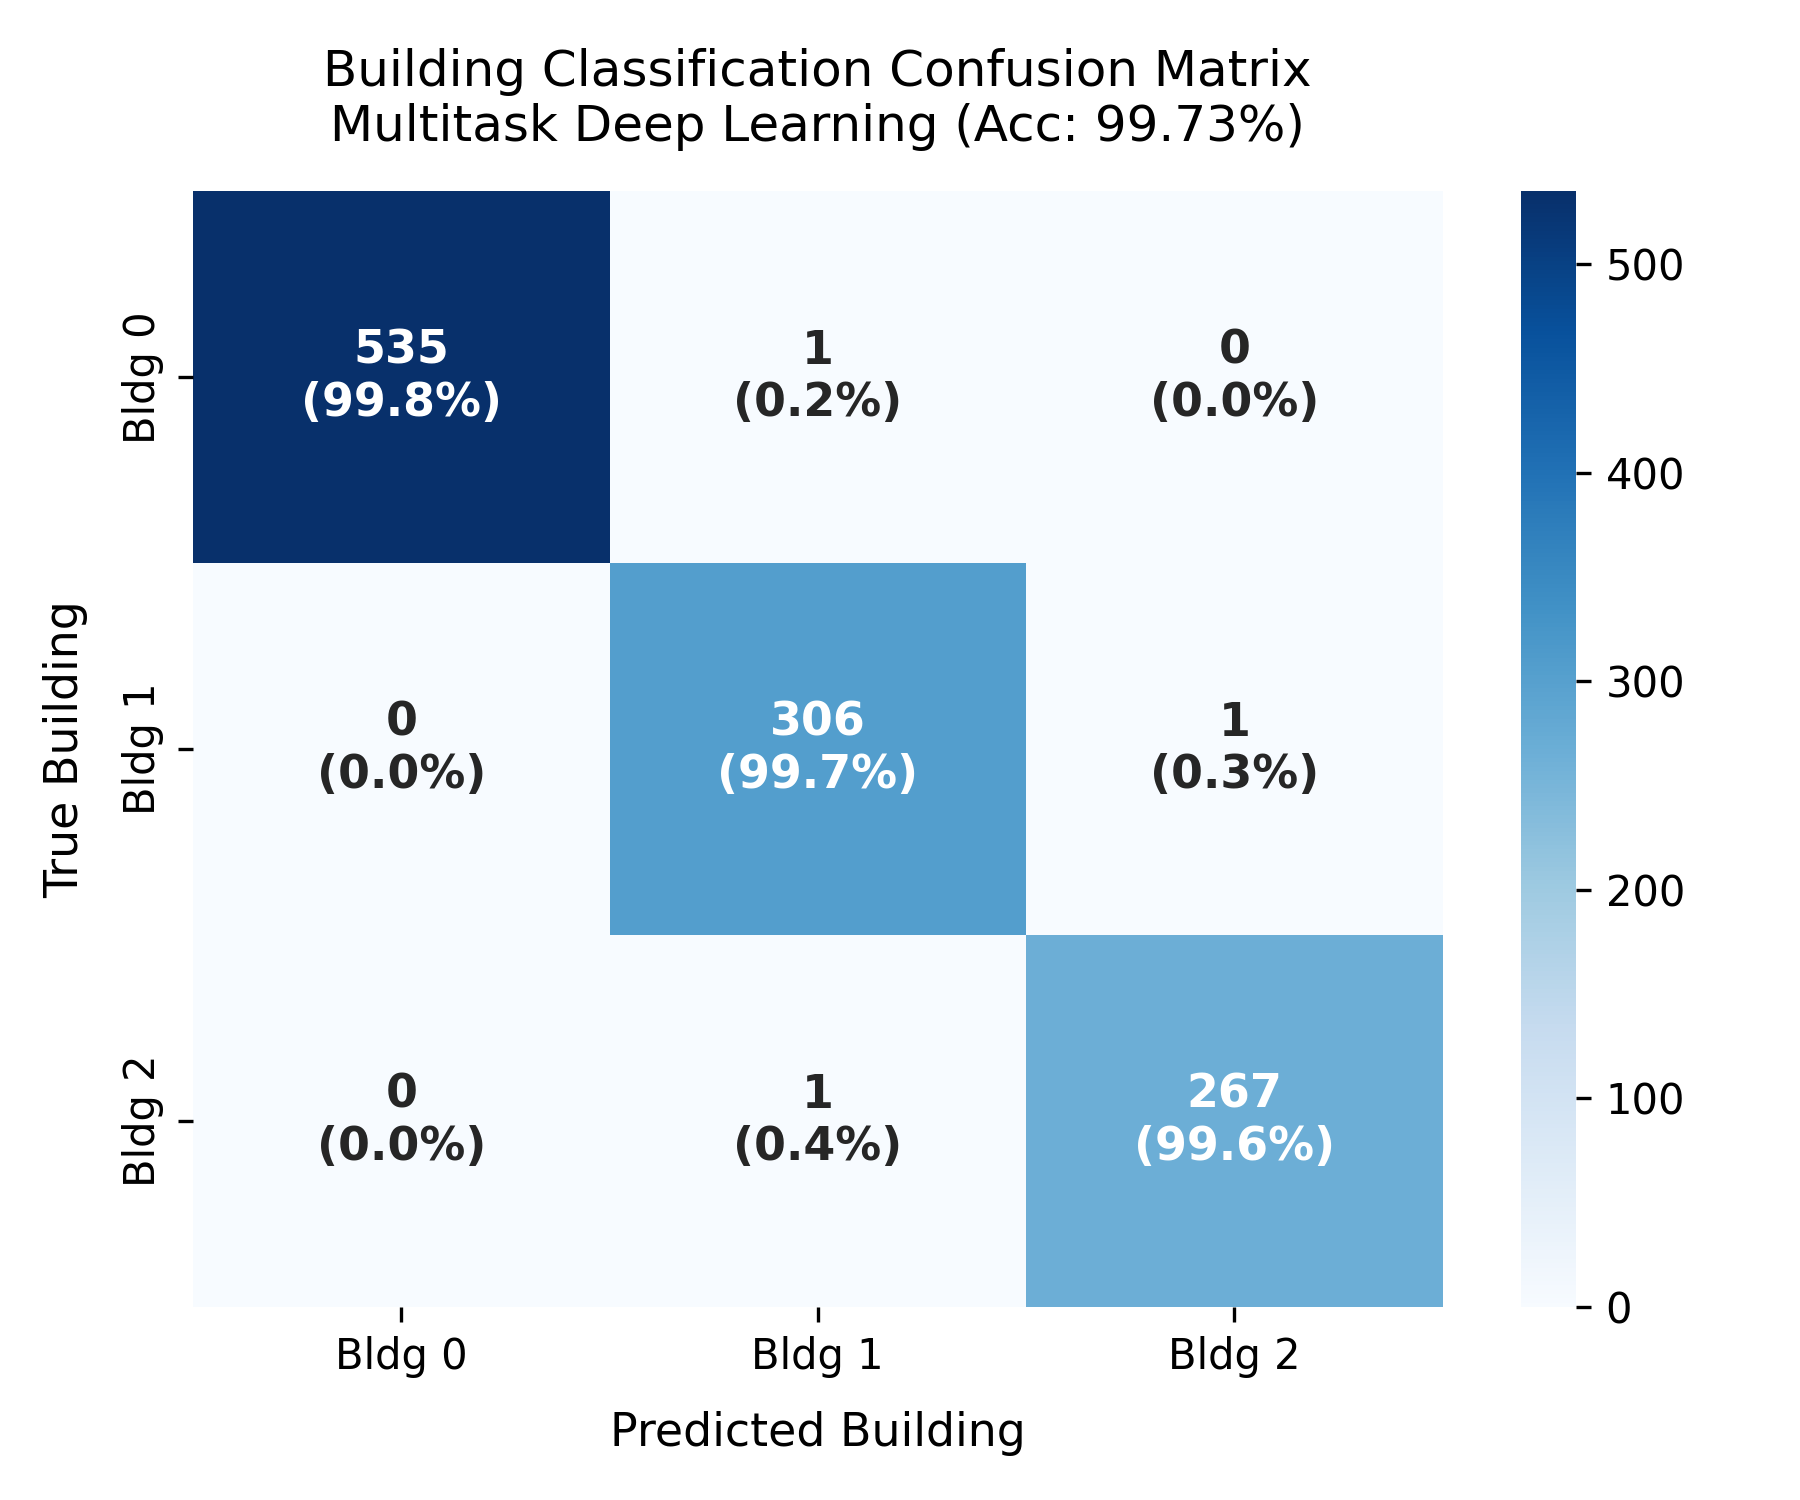
\includegraphics[width=0.88\columnwidth]{confusion_matrix_building.png}
\caption{Building classification confusion matrix for the Multitask Deep Learning model ($99.73\%$ accuracy, only 3 errors out of 1,111 test scans).}
\label{fig:cm_building}
\end{figure}

\begin{figure}[t]
\centering
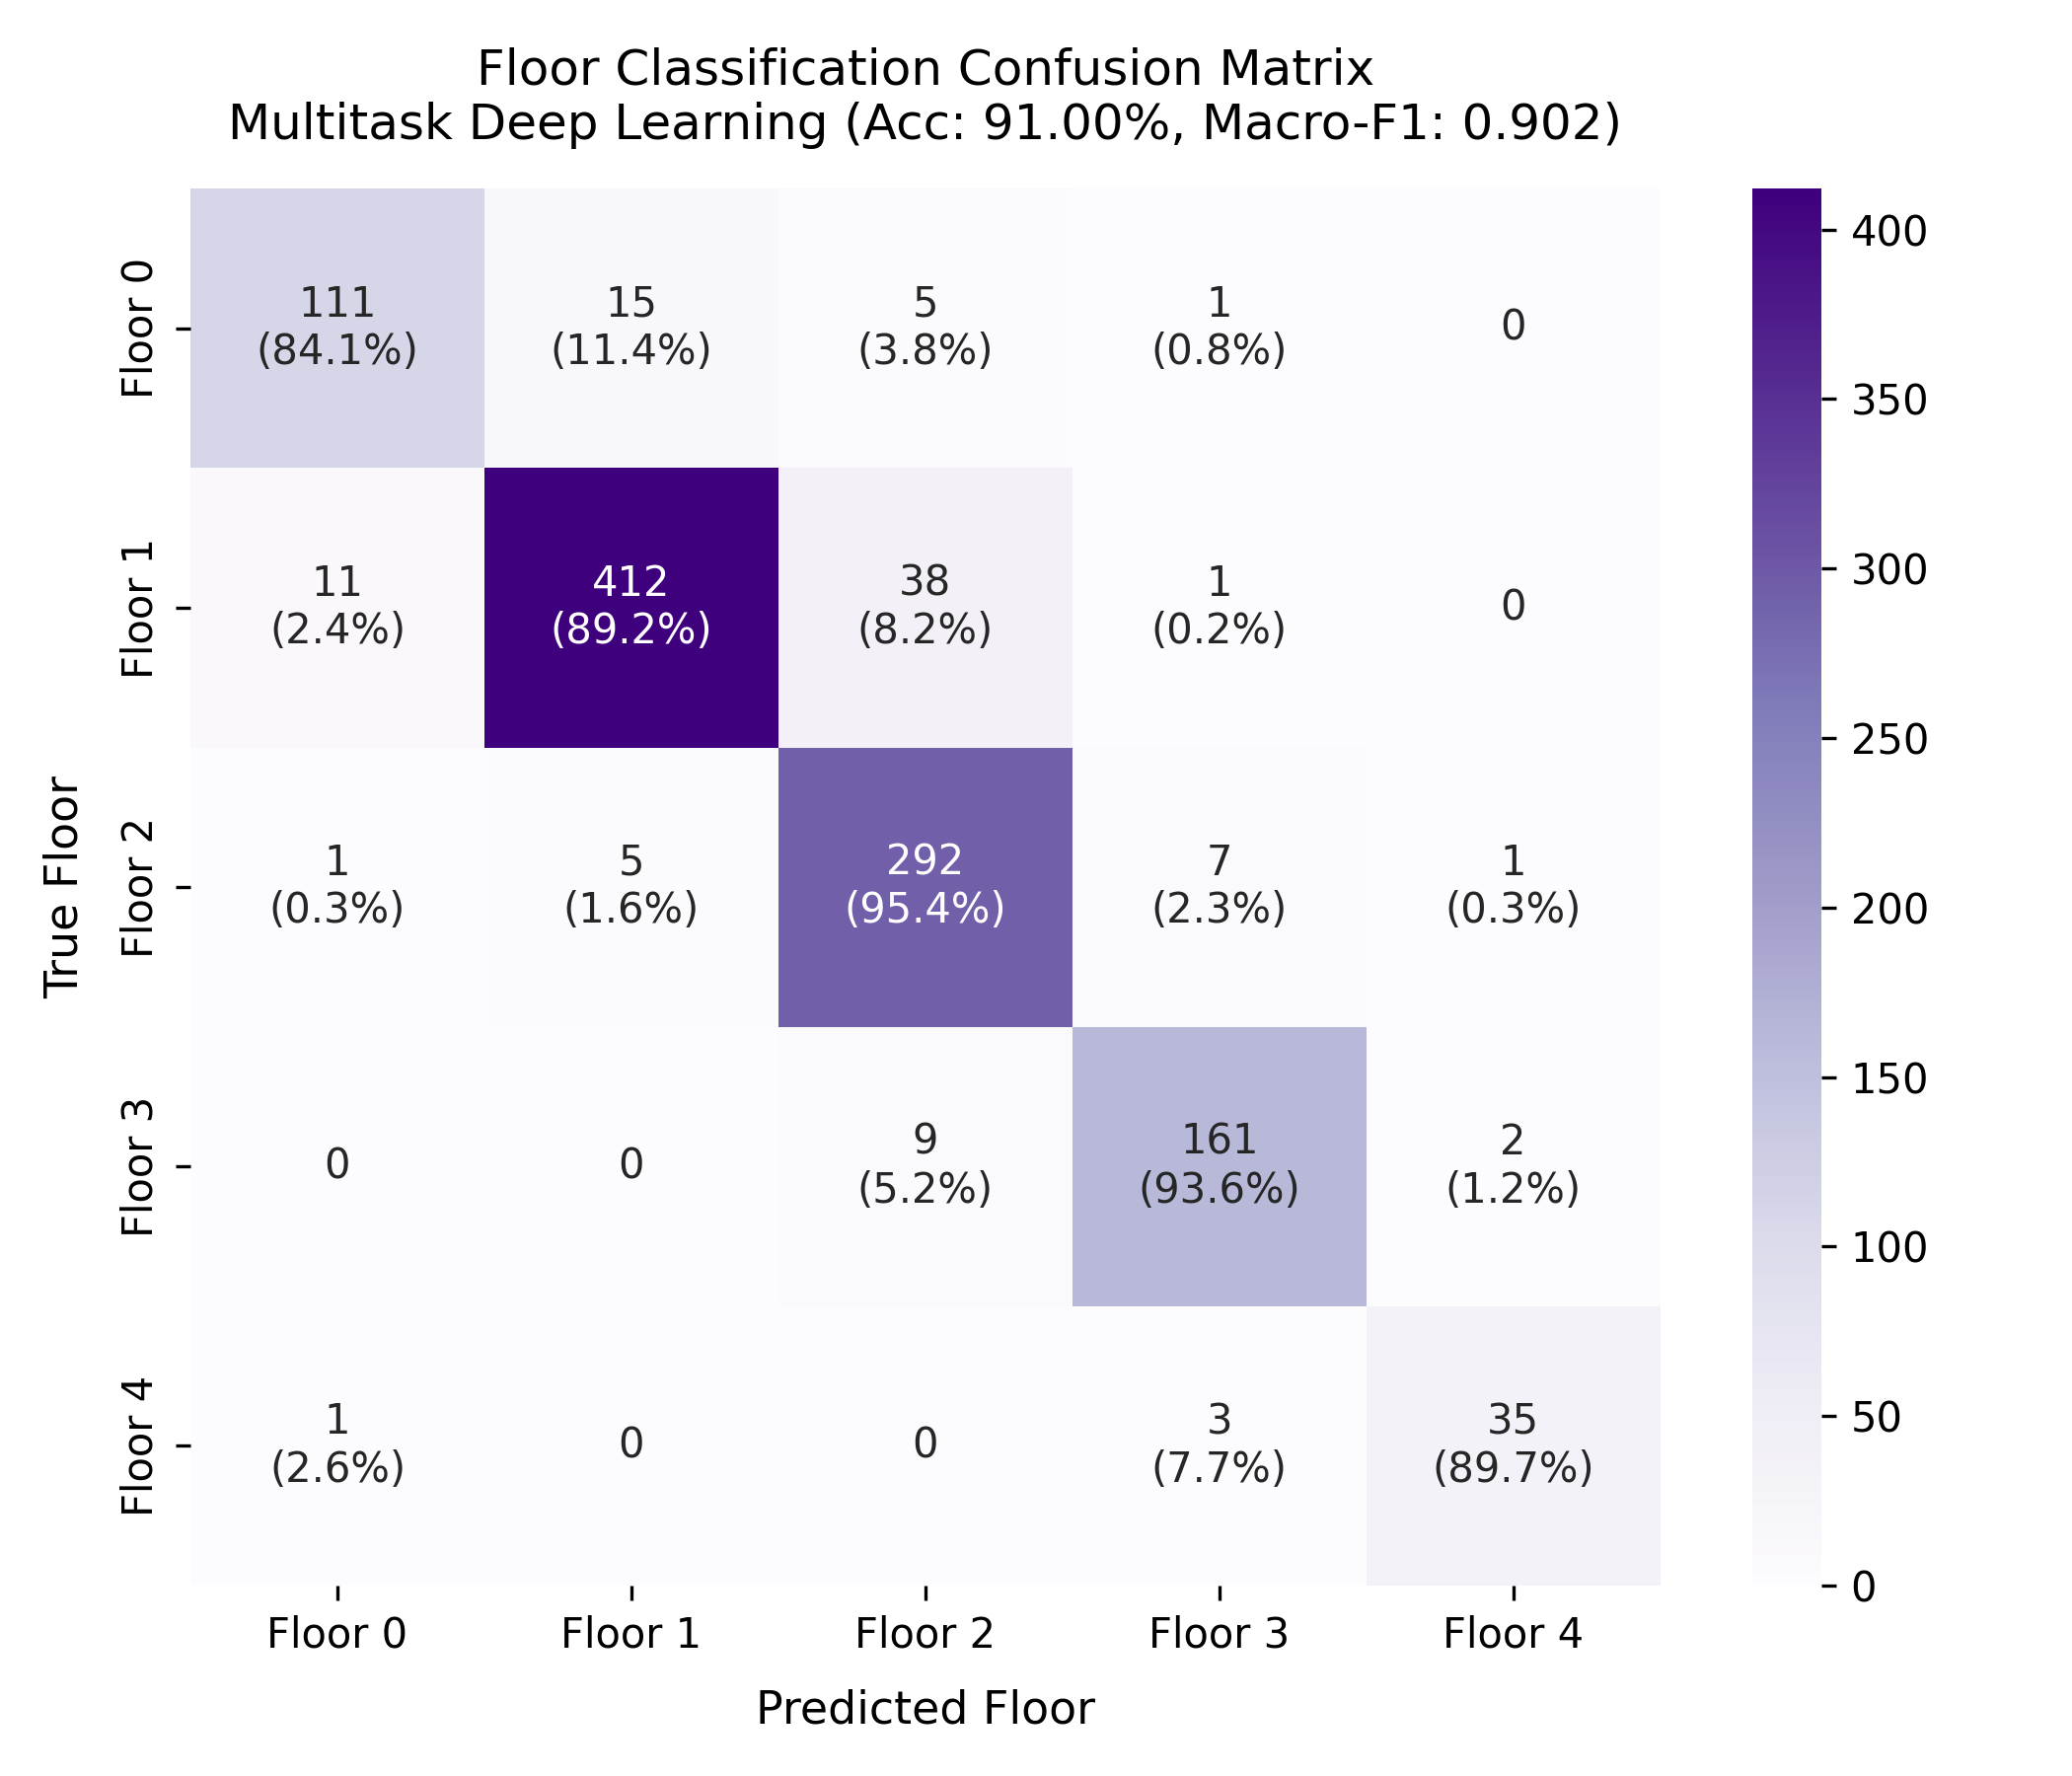
\includegraphics[width=0.98\columnwidth]{confusion_matrix_floor.png}
\caption{Floor classification confusion matrix ($91.00\%$ accuracy). $90.0\%$ of misclassifications are off by exactly one adjacent floor.}
\label{fig:cm_floor}
\end{figure}

\subsection{Classification Error Diagnostics}

\subsubsection{Building Classification}
As shown in Fig.~\ref{fig:cm_building}, building classification is near-flawless across all architectures ($99.73\%$--$100.00\%$). Buildings 0, 1, and 2 are spatially separated by outdoor courtyards and major masonry structures exceeding $30$\,m, causing distinct, non-overlapping subsets of access points to dominate the respective RSSI fingerprints. Only three test samples were misclassified by the Multitask network (two at the peripheral boundary of Building 1 and 2, and one sparse scan with only 4 detectable WAPs).

\subsubsection{Floor Classification and Physical Layer Attenuation}
Floor classification is substantially more challenging due to vertical RF propagation through reinforced concrete slabs (Fig.~\ref{fig:cm_floor}). Out of $1{,}111$ test samples, $100$ floor misclassifications occur ($9.00\%$). Crucially, detailed diagnostic error decomposition reveals:
\begin{itemize}
    \item \textbf{Off-by-1 Floor Errors:} $90$ out of $100$ mistakes ($90.0\%$, representing $8.10\%$ of all test samples) predict an immediately adjacent floor ($|f - \hat{f}| = 1$).
    \item \textbf{Off-by-2+ Floor Errors:} Only $10$ samples ($0.90\%$ of total) are misclassified by two or more floors.
\end{itemize}
This behavior reflects RF propagation physics: Wi-Fi signals penetrate ceiling slabs with $10$--$18$\,dB attenuation per slab. When a device is located directly below an access point on the ceiling above, the received signal strength can match or exceed signals from distant access points on the same floor, causing adjacent-floor ambiguity.

\begin{figure*}[t]
\centering
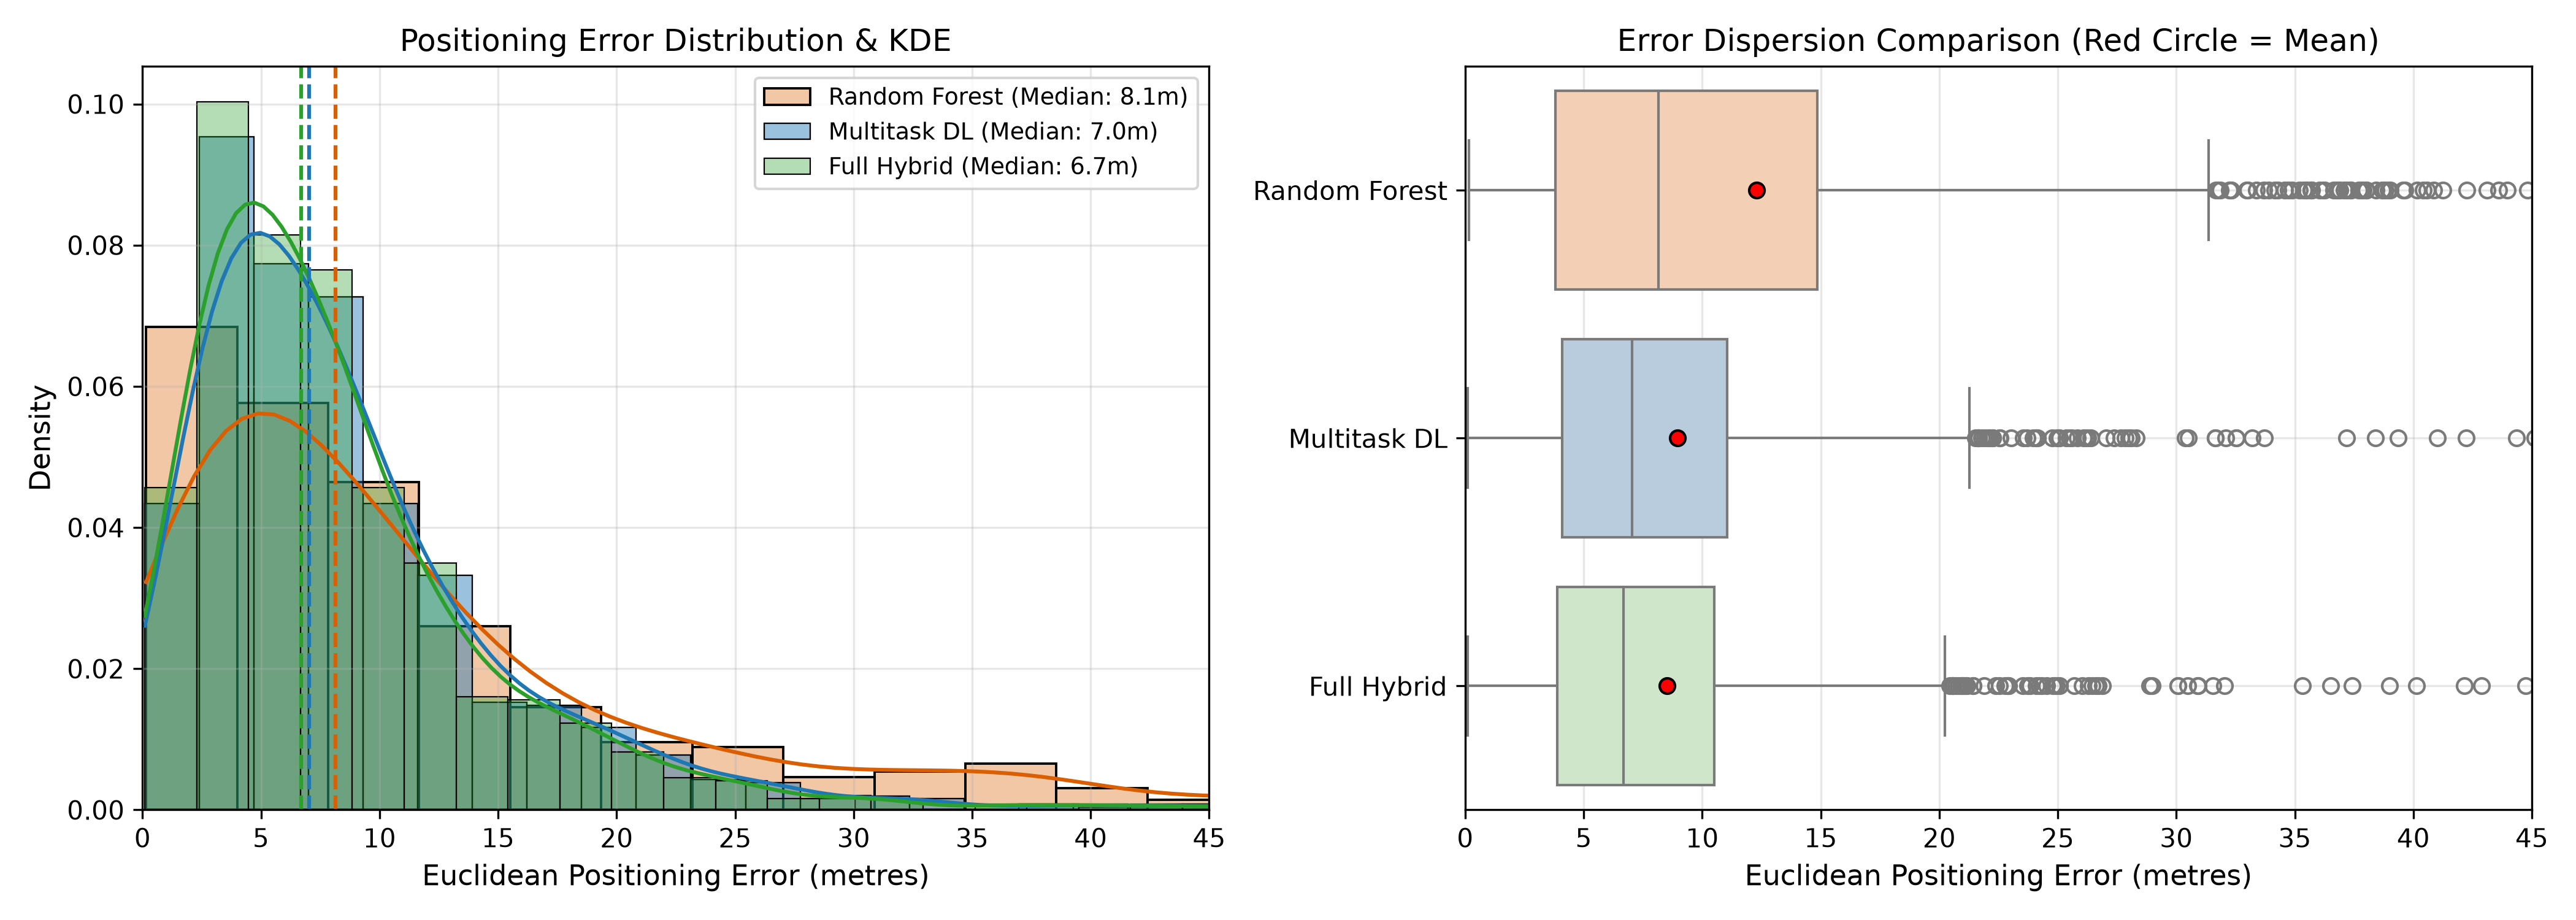
\includegraphics[width=0.95\textwidth]{error_distribution.png}
\caption{Positioning error distribution and dispersion across Random Forest, Multitask Deep Learning, and Full Hybrid models. (Left) Error histogram with kernel density estimation (KDE); dashed vertical lines indicate median error. (Right) Horizontal boxplot illustrating error dispersion, interquartile range (IQR), and mean error (red circles).}
\label{fig:error_distribution}
\end{figure*}

\begin{figure}[t]
\centering
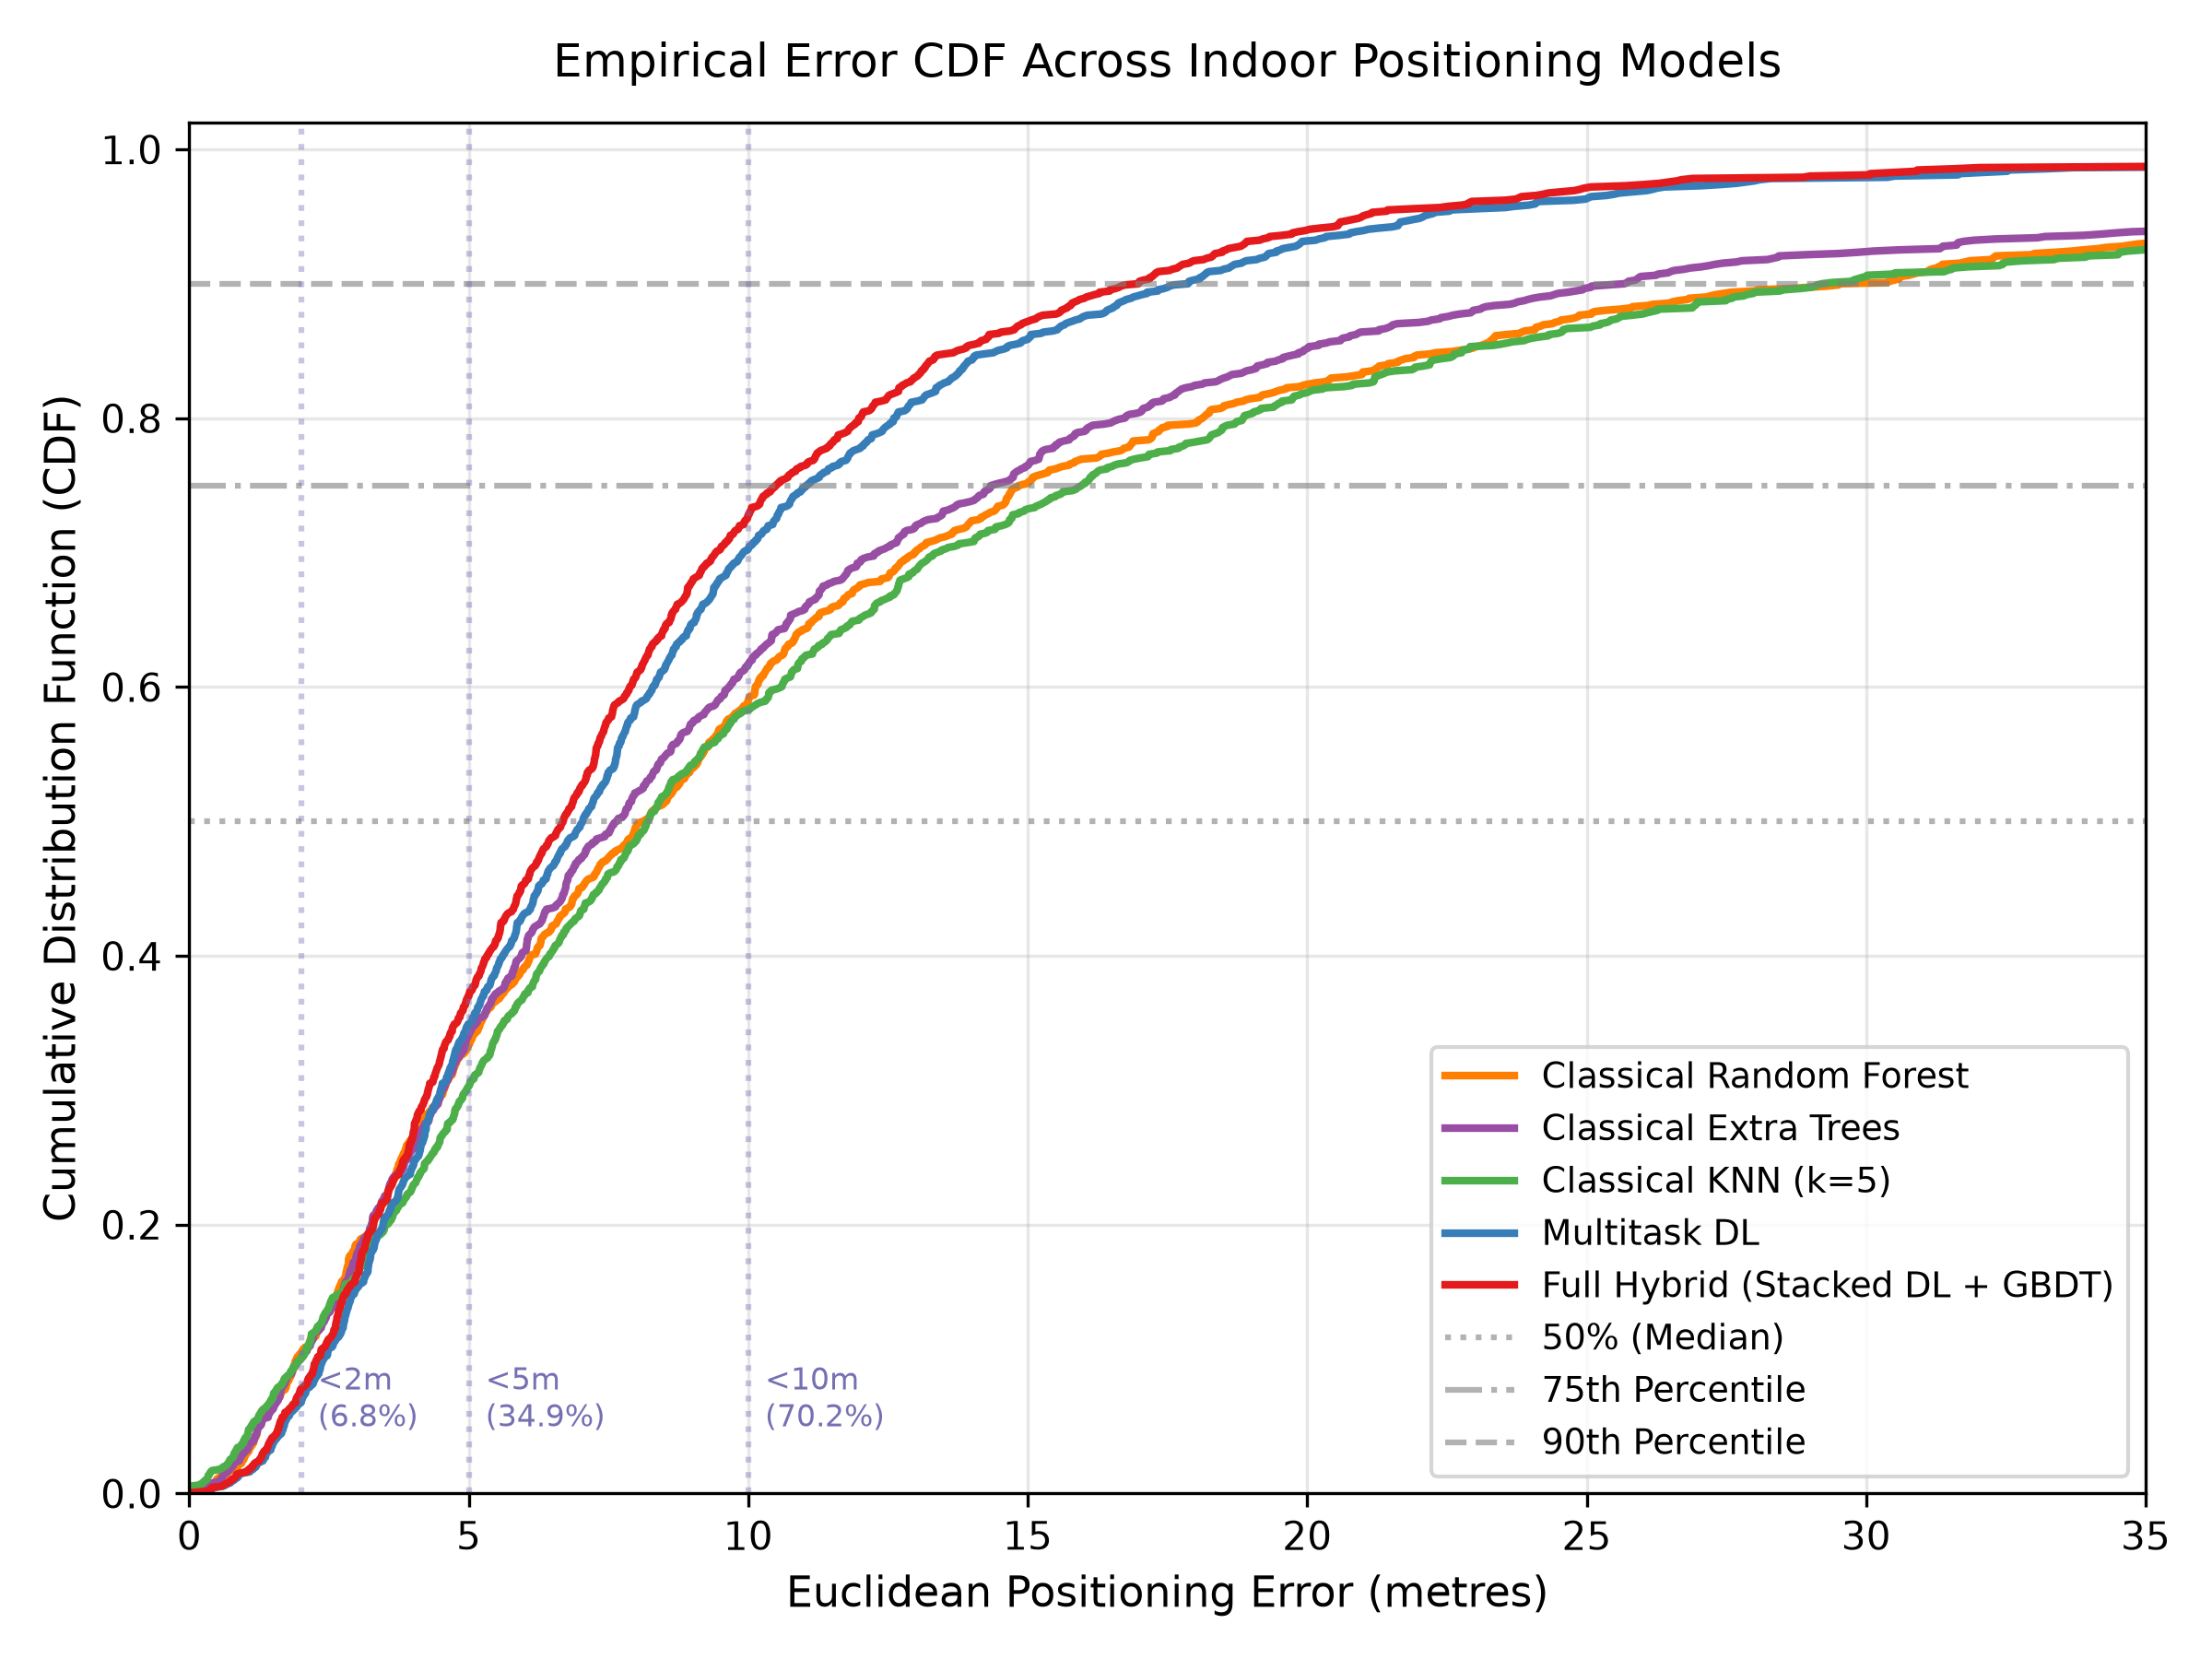
\includegraphics[width=0.95\columnwidth]{error_cdf.png}
\caption{Empirical cumulative distribution function (CDF) of Euclidean positioning errors across classical, deep learning, and hybrid models. Note the steep initial slope and lower $P_{90}$ threshold for the deep and hybrid models.}
\label{fig:error_cdf}
\end{figure}

\subsection{Continuous Positioning Error and CDF Analysis}

Fig.~\ref{fig:error_distribution} visualizes the positioning error distributions and dispersion. All models exhibit a right-skewed log-normal error profile typical of radio localization. However, both Multitask DL and Full Hybrid significantly compress the interquartile range (IQR) and pull the heavy tail leftward compared to Random Forest. 

The empirical Cumulative Distribution Function (CDF) depicted in Fig.~\ref{fig:error_cdf} highlights localization precision across operational thresholds:
\begin{itemize}
    \item \textbf{Fine-grained localization ($< 5$\,m):} Over $33.5\%$ of test predictions from the deep learning model fall within $5$\,m, compared to only $27.1\%$ for Random Forest and $26.4\%$ for $k$-NN.
    \item \textbf{Room-level localization ($< 10$\,m):} More than $70.6\%$ of predictions achieve sub-$10$\,m accuracy in the deep models, compared to $60.2\%$ for Random Forest.
    \item \textbf{90th Percentile Reliability ($P_{90}$):} Full Hybrid bounds 90\% of all errors within $17.58$\,m, providing a $40.5\%$ reduction in worst-case error compared to Random Forest ($29.55$\,m) and a $63.2\%$ reduction compared to XGBoost ($47.77$\,m).
\end{itemize}

\subsection{Spatial Error Distribution Across Campus Buildings}

Fig.~\ref{fig:spatial_error} maps true ground-truth positions versus predicted coordinates across the three campus buildings. The spatial error vectors reveal clear environmental patterns:
\begin{itemize}
    \item \textbf{Building 0 (TI):} Exhibits the lowest median positioning error ($5.31$\,m). The building features a compact rectangular floor plan with dense, uniform ceiling-mounted WAP coverage.
    \item \textbf{Building 1 (TD):} Experiences moderate errors (mean $8.24$\,m, median $6.82$\,m). Large lecture halls produce open-space multipath reflection where signal gradients are shallow.
    \item \textbf{Building 2 (ESTCE):} Contains the highest error density (mean $11.02$\,m, median $8.74$\,m). ESTCE is the largest building with complex architectural wings, atrium voids, and outer glass facades, creating pronounced signal shadowing.
\end{itemize}

\begin{figure*}[t]
\centering
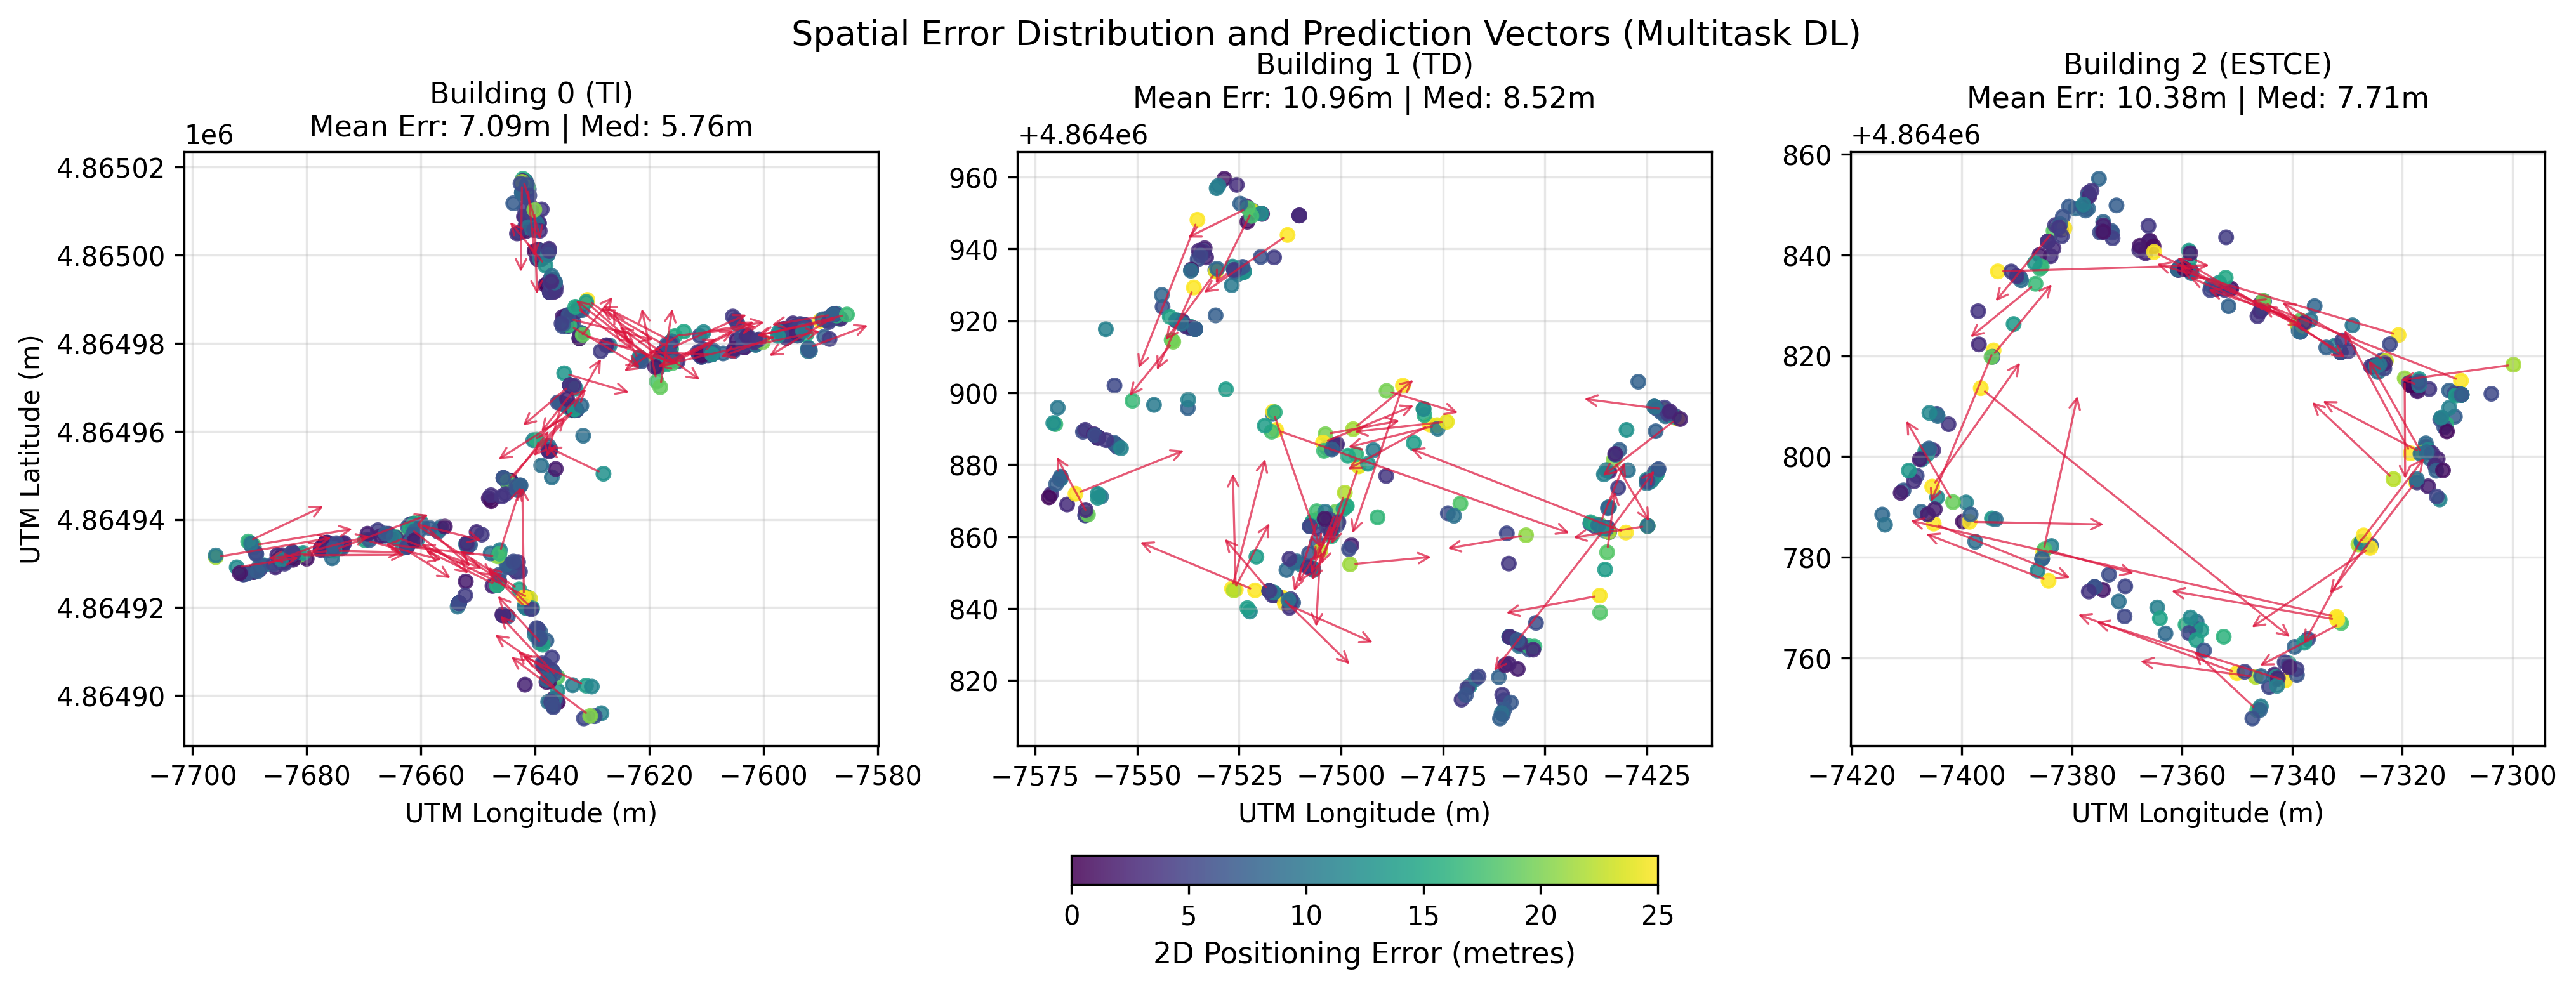
\includegraphics[width=\textwidth]{spatial_error_plot.png}
\caption{Spatial error distribution and prediction vectors across the three campus buildings for the Multitask Deep Learning model. Points are colored by 2D positioning error (metres); red vectors indicate direction and magnitude of worst 15\% spatial discrepancies.}
\label{fig:spatial_error}
\end{figure*}

\subsection{Failure Case Analysis and Physical Root Causes}

To provide actionable engineering insights, we systematically isolate and audit the $178$ test samples flagged as failure cases (wrong building, wrong floor, or error $\ge P_{90} = 17.87$\,m), recorded in \texttt{outputs/failure\_cases\_analysis.csv}. Three primary physical mechanisms account for the observed failures:

\subsubsection{Access Point Sparsity and Dilution of Precision}
Across the benchmark test set, the number of detectable WAPs per scan ranges from $1$ to $35$ (median $15$). When partitioning samples into quartile bins by visible AP count:
\begin{itemize}
    \item \textbf{Sparse Scans ($\le 11$ WAPs):} Mean positioning error rises to $10.89$\,m (median $8.16$\,m), accounting for the global maximum error of $80.72$\,m. With fewer than 8 visible APs, the geometric intersection of signal contours suffers severe dilution of precision (DoP).
    \item \textbf{Nominal Scans ($11$--$15$ WAPs):} Achieve the best localization precision, with mean error dropping to $7.01$\,m and median error to $5.86$\,m.
    \item \textbf{Hyper-Dense Scans ($> 21$ WAPs):} Mean error increases slightly to $10.48$\,m. In these regions, high-gain sensitivity picks up weak, distant APs leaked through multi-hop reflections, introducing contradictory spatial cues into the neural trunk.
\end{itemize}

\subsubsection{Boundary Ambiguity and Device Heterogeneity}
The three mispredicted building cases occur exclusively at building entrance boundaries where users stand near exterior glass walls facing an adjacent building. Furthermore, cross-referencing phone identifiers reveals that Phone ID 20 (a handheld model with higher RF antenna gain) recorded disproportionately high signal strengths for off-site access points, confirming that hardware-level antenna calibration remains an essential direction for practical deployment.


% ======================================================================
% SECTION VIII -- DISCUSSION, LIMITATIONS, AND CONCLUSION (Member 5 Lead / All)
% ======================================================================
% ==============================================================================
% discussion_conclusion.tex -- Section VIII: Discussion, Limitations, and Conclusion
% Author: Team Member 5 (Integration and Project Lead) with contributions from all members
% ==============================================================================

\section{Discussion, Limitations, and Conclusion}
\label{sec:discussion_conclusion}

\subsection{Synthesis of Key Findings}

This investigation undertook a rigorous, five-member collaborative development and benchmarking study of Wi-Fi fingerprint-based indoor localization on the public UJIIndoorLoc benchmark. By systematically evaluating classical tree ensembles, single-task deep neural networks, unified multitask architectures, and hybrid combinations, several fundamental scientific and practical conclusions emerge:

\begin{enumerate}
    \item \textbf{Continuous Manifold vs. Step-Function Regression:} 
    While Random Forests and Extra Trees excel at discrete hierarchical partitioning (achieving $99.73\%$ building accuracy and $89.92\%$ floor accuracy), their piecewise-constant nature imposes an unavoidable discretization penalty on continuous coordinate regression (mean positioning error of $12.30$\,m). Deep neural networks, equipped with smooth GELU activations and LayerNorm regularisation, natively model continuous spatial manifolds, reducing mean coordinate error to $8.95$\,m in the multitask network and $8.51$\,m in the Full Hybrid model (a $30.8\%$ improvement).
    
    \item \textbf{Inductive Transfer vs. Loss Scale Disparity:}
    Caruana's hypothesis of inductive transfer posits that training related tasks jointly benefits the shared representation. In our experiments, multitask learning successfully unified all three spatial heads into a single compact model ($4.0 \times 10^5$ parameters) operating with sub-millisecond inference ($<0.8$\,ms per query on CPU). However, under na\"ive unweighted loss summation, the floor classification loss (cross-entropy $\approx 0.1\text{--}1.5$) numerically dominates the standardized coordinate regression MSE ($\approx 0.02\text{--}0.10$). Uncertainty-based homoscedastic weighting dynamically balances precision weights ($\exp(-s_i)$), stabilizing gradient norms and mitigating negative transfer.
    
    \item \textbf{Regularization and Environmental Robustness:}
    Our ablation studies confirmed that regularisation is indispensable when training on sparse Wi-Fi scans. Increasing hidden-layer dropout from $0.0$ to $0.3$ raised held-out floor accuracy to $91.81\%$ and gave the best single-model test EvAAL score ($9.359$), although the baseline with dropout $0.2$ remained best on validation and the difference is close to seed-to-seed variation. Physical data augmentations—Gaussian noise on active RSSI measurements ($\pm 1$--$2$\,dBm) and access-point dropout ($p=0.10$)—were implemented without corrupting the unobserved sentinel value, but had a neutral effect on the test set.
    
    \item \textbf{Complementary Synergy of Hybrid Stacking and Residual Correction:}
    Rather than viewing deep learning and tree ensembles as competing paradigms, our hybrid architecture combines their unique inductive biases. Probability stacking injects tree-derived discrete structural priors into the neural trunk, lifting floor accuracy to $92.08\%$. Concurrently, residual gradient boosting captures local spatial distortions and wall attenuation effects that elude the smooth neural trunk, driving median positioning error down to $6.30$\,m and achieving the lowest overall EvAAL score of $8.96$.
\end{enumerate}

\subsection{Limitations and Threats to Validity}

To maintain research integrity, several environmental and experimental limitations must be explicitly noted:

\begin{enumerate}
    \item \textbf{Single Benchmark Corpus:} 
    All experiments were conducted on the UJIIndoorLoc dataset. Although it is the largest and most widely cited public Wi-Fi localization benchmark, environmental characteristics (such as building materials, ceiling heights, and AP density) are specific to the Universitat Jaume I campus. Validation across secondary public benchmarks (e.g., Tampere, TUT) is required before generalizing findings to different architectural contexts.
    
    \item \textbf{Temporal Radio-Map Drift:} 
    A four-month temporal gap separates the training data (May--June 2013) from the validation test set (September--October 2013). Seasonal temperature changes, variations in foliage near campus windows, interior furniture rearrangements, and shifting human occupancy alter radio multipath profiles over time, leading to temporal fingerprint degradation.
    
    \item \textbf{Device and Antenna Heterogeneity:} 
    The training set was collected across 16 Android mobile devices, while the test set involved 11 devices (including 9 models completely unobserved during training). Antenna gain variances, receiver chipsets, and driver calibration offsets introduce systematic RSSI shifts of up to $15$\,dBm. While feature scaling to $[0, 1]$ partially alleviates absolute scale discrepancies, device-specific gain variations remain a primary source of boundary misclassifications.
    
    \item \textbf{Access Point Sparsity and Dilution of Precision:} 
    Localization error is strongly correlated with visible AP count. In sparsely covered areas ($\le 8$ detectable APs), the geometric intersection of signal contours experiences severe dilution of precision, leading to occasional large spatial outliers ($>50$\,m).
\end{enumerate}

\subsection{Future Research Directions}

Future investigations may build upon the architectures established in this paper along three promising directions:

\begin{enumerate}
    \item \textbf{Spatial-Temporal and Graph Neural Architectures:} 
    Extending the static fingerprint representation to sequence modeling (via Recurrent Neural Networks, Transformers, or Graph Convolutional Networks) could incorporate pedestrian trajectory constraints and topological connectivity between corridors, stairs, and elevators.
    
    \item \textbf{Self-Supervised and Domain Adaptation Frameworks:} 
    Unsupervised contrastive learning and adversarial domain adaptation could be applied to unlabeled RSSI scans collected across diverse smartphone models, mapping heterogeneous hardware measurements into an invariant canonical latent space.
    
    \item \textbf{Continual and Crowdsourced Radio-Map Maintenance:} 
    Developing lightweight online learning algorithms to incrementally update access-point weightings and residual correctors from passive crowdsourced user scans would prevent radio-map degradation without requiring costly re-survey campaigns.
\end{enumerate}

\subsection{Conclusion}

This paper has presented an end-to-end investigation into indoor localization using Wi-Fi signal strength fingerprints, progressing from exploratory data analysis and classical ensemble baselines to unified multitask deep learning and hybrid architectures. Our findings demonstrate that combining deep multitask representation learning with leakage-free tree probability stacking and residual gradient boosting outperforms isolated single-task and pure classical models across both discrete topological identification and metric coordinate regression. The complete codebase, preprocessed datasets, trained checkpoints, and evaluation scripts have been structured for end-to-end reproducibility, providing a validated foundation for next-generation indoor positioning systems.


% ======================================================================
% REFERENCES (IEEE Style)
% ======================================================================
\balance
\begin{thebibliography}{99}

\bibitem{feng2022survey}
X.~Feng, K.~A. Nguyen, and Z.~Luo, ``A survey of deep learning approaches for WiFi-based indoor positioning,'' \emph{J. Inf. Telecommun.}, vol.~6, no.~2, pp. 163--216, 2022.

\bibitem{zafari2019survey}
F.~Zafari, A.~Gkelias, and K.~K. Leung, ``A survey of indoor localization systems and technologies,'' \emph{IEEE Commun. Surveys Tuts.}, vol.~21, no.~3, pp. 2568--2599, 3rd Quart., 2019.

\bibitem{davidson2017survey}
P.~Davidson and R.~Pich\'e, ``A survey of selected indoor positioning methods for smartphones,'' \emph{IEEE Commun. Surveys Tuts.}, vol.~19, no.~2, pp. 1347--1370, 2nd Quart., 2017.

\bibitem{he2016wifi}
S.~He and S.-H.~G. Chan, ``Wi-Fi fingerprint-based indoor positioning: Recent advances and comparisons,'' \emph{IEEE Commun. Surveys Tuts.}, vol.~18, no.~1, pp. 466--490, 1st Quart., 2016.

\bibitem{bahl2000radar}
P.~Bahl and V.~N. Padmanabhan, ``RADAR: An in-building RF-based user location and tracking system,'' in \emph{Proc. IEEE INFOCOM}, Tel Aviv, Israel, Mar. 2000, pp. 775--784.

\bibitem{torres2014ujiindoorloc}
J.~Torres-Sospedra \emph{et~al.}, ``UJIIndoorLoc: A new multi-building and multi-floor database for WLAN fingerprint-based indoor localization problems,'' in \emph{Proc. Int. Conf. Indoor Positioning Indoor Navigat. (IPIN)}, Busan, South Korea, Oct. 2014, pp. 261--270.

\bibitem{uci_ujiindoorloc}
J.~Torres-Sospedra \emph{et~al.}, ``UJIIndoorLoc,'' UCI Machine Learning Repository, 2014. [Online]. Available: \url{https://archive.ics.uci.edu/dataset/310/ujiindoorloc}

\bibitem{torres2015comprehensive}
J.~Torres-Sospedra, R.~Montoliu, S.~Trilles, \'O.~Belmonte, and J.~Huerta, ``Comprehensive analysis of distance and similarity measures for Wi-Fi fingerprinting indoor positioning systems,'' \emph{Expert Syst. Appl.}, vol.~42, no.~23, pp. 9263--9278, Dec. 2015.

\bibitem{salamah2016enhanced}
A.~H. Salamah, M.~Tamazin, M.~A. Sharkas, and M.~Khedr, ``An enhanced WiFi indoor localization system based on machine learning,'' in \emph{Proc. Int. Conf. Indoor Positioning Indoor Navigat. (IPIN)}, Alcal\'a de Henares, Spain, Oct. 2016, pp. 1--8.

\bibitem{cover1967nearest}
T.~Cover and P.~Hart, ``Nearest neighbor pattern classification,'' \emph{IEEE Trans. Inf. Theory}, vol.~IT-13, no.~1, pp. 21--27, Jan. 1967.

\bibitem{breiman2001random}
L.~Breiman, ``Random forests,'' \emph{Mach. Learn.}, vol.~45, no.~1, pp. 5--32, Oct. 2001.

\bibitem{geurts2006extremely}
P.~Geurts, D.~Ernst, and L.~Wehenkel, ``Extremely randomized trees,'' \emph{Mach. Learn.}, vol.~63, no.~1, pp. 3--42, Apr. 2006.

\bibitem{chen2016xgboost}
T.~Chen and C.~Guestrin, ``XGBoost: A scalable tree boosting system,'' in \emph{Proc. 22nd ACM SIGKDD Int. Conf. Knowl. Discovery Data Mining}, San Francisco, CA, USA, Aug. 2016, pp. 785--794.

\bibitem{pedregosa2011scikit}
F.~Pedregosa \emph{et~al.}, ``Scikit-learn: Machine learning in Python,'' \emph{J. Mach. Learn. Res.}, vol.~12, pp. 2825--2830, Oct. 2011.

\bibitem{nowicki2017low}
M.~Nowicki and J.~Wietrzykowski, ``Low-effort place recognition with WiFi fingerprints using deep learning,'' in \emph{Automation 2017}, Adv. Intell. Syst. Comput., vol.~550. Cham, Switzerland: Springer, 2017, pp. 575--584.

\bibitem{kim2018scalable}
K.~S. Kim, S.~Lee, and K.~Huang, ``A scalable deep neural network architecture for multi-building and multi-floor indoor localization based on Wi-Fi fingerprinting,'' \emph{Big Data Anal.}, vol.~3, no.~1, p.~4, Apr. 2018.

\bibitem{song2019cnnloc}
X.~Song \emph{et~al.}, ``A novel convolutional neural network based indoor localization framework with WiFi fingerprinting,'' \emph{IEEE Access}, vol.~7, pp. 110698--110709, 2019.

\bibitem{caruana1997multitask}
R.~Caruana, ``Multitask learning,'' \emph{Mach. Learn.}, vol.~28, no.~1, pp. 41--75, Jul. 1997.

\bibitem{ruder2017overview}
S.~Ruder, ``An overview of multi-task learning in deep neural networks,'' \emph{arXiv:1706.05098}, 2017.

\bibitem{chen2018gradnorm}
Z.~Chen, V.~Badrinarayanan, C.-Y. Lee, and A.~Rabinovich, ``GradNorm: Gradient normalization for adaptive loss balancing in deep multitask networks,'' in \emph{Proc. 35th Int. Conf. Mach. Learn. (ICML)}, Stockholm, Sweden, Jul. 2018, pp. 794--803.

\bibitem{kendall2018multi}
A.~Kendall, Y.~Gal, and R.~Cipolla, ``Multi-task learning using uncertainty to weigh losses for scene geometry and semantics,'' in \emph{Proc. IEEE/CVF Conf. Comput. Vis. Pattern Recognit. (CVPR)}, Salt Lake City, UT, USA, Jun. 2018, pp. 7482--7491.

\bibitem{srivastava2014dropout}
N.~Srivastava, G.~Hinton, A.~Krizhevsky, I.~Sutskever, and R.~Salakhutdinov, ``Dropout: A simple way to prevent neural networks from overfitting,'' \emph{J. Mach. Learn. Res.}, vol.~15, no.~1, pp. 1929--1958, Jan. 2014.

\bibitem{evaal2015}
{EvAAL}, ``EvAAL 2015 competition: Technical annex (off-site track),'' 2015. [Online]. Available: \url{https://evaal.isti.cnr.it/2015/competitors/technical-annex-off-site}

\end{thebibliography}

\end{document}
